\documentclass[phd]{ndsu-thesis-2022} 

%------------------------------------------------------------------------------
%-------------[Options]-applicable in this class----------------------
% Degree options (any of these):  phd, ms-thesis, ms-paper, ma-thesis, ma-paper, default is phd; 
% Whole document font size (any of these): 10pt, 11pt, 12pt, default = 12pt; 
% nonumber = document without chapter/section numbering - one of the NDSU template style, default = numbered, tables and figures are serially numbered;
% chapternumber = document with only chapter numbering and no number of other sections, tables and figures are numbered with chapter numbers;
% nojustify = ragged-right (non-hyphenated whole words) passages, default = justified (hyphenated words) with straight right margin; 
% draft = no figures but box frames, default = final; 
% showframe = frame around the text area to check how text fills in the margins - this with draft option shows the items crossing the frame, default = noshowframe; 
% showgrid = grid around the text area to check the vertical spacing of elements to adjust the spacing to match the double-line spacing
% fonts (any of these): bookman, charter, gentium, kpfonts, libertine, mathdesign, mathptmx, newcent, palatino, tgtermes, times, tgbonum, tgpagella, tgschola, utopia, zlmtt, default = LaTeX computer modern. 
% chapterrefs = individual reference sections, default = combined reference unnumbered chapter; with this option need to use \checkBeginRefsection, \checkEndRefsection (for each chapter) and \checkMakeCombinedReferences once at the end (refer ndsu-sandbox-asabe.tex)
%------------------------------------------------------------------------------

%---------------------------------------------------------------------------------------------------
% --------------Other useful commands or shortcuts available are:-----------------
% \listofabbreviations  = A 2-col tabular environment; Usage: {SI & System International}\\
% \listofsymbols =  A 2-col tabular environment; Usage: {$A$ &  Area (\si{\m\squared})}\\
% \tempend{*.sty}{*.bib}  =  temporarily ending the document with reference listing
% \myspacing =  defined to give the correct spacing of about 23 lines per page
% \myheading = proper numbering and format
% \si{} and \SI{}{} = SI units from siunitx package that gives proper spacing between numbers and units
% \citep and \citet = natbib package commands application with options
% \myfig{5 items} = shortcut for regular figures {placement}{size}{file}{caption}{label}
% \myfigls {5 items} = shortcut for landscape figures {placement}{size}{file}{caption}{label}
% \cref and \Cref = use of cleveref package based reference
% \tabcolsep = to stretch the tables to fill the entire width
% \resizebox = to adjust the size of tables to fit the margins (font size will change)
% \toprule, \midrule, \cmidrule, \bottomrule = booktabs package commands for tables
% tablenotes env. =  threeparttable package commands for tables with footnotes 
% longtable env. = for longer tables that spans several pages from longtable package - can be combined with threeparttable t
% \abovedisplayskip = to adjust the space above the displayed items
% \hl, \nt, \dt, \rt, \notes = annotation commands: highlight, new text, delete text, replace text, and todo notes
% \url = URLs break well as expected at the right margin (necessary code added in class)
% \namedappendices{A}{Name ... } = multiple appendices - correctly producing all elements
% \myfigap, \myfigapls = appendix regular figure and appendix landscape figure {5 items as before}
% \citestyle{} = predefined natbib styles (options: plain, agu, egu, agms, dcu, kluwer, cospar, nature) use this after \usepackage[sort&compress]{natbib}
% \lstset{e.g. language, font, style, color} options and {lstlisting} environment of listings package for programs and algorithms source code listing
% \tendc = can be used to temporarily end the document (BibLaTeX individual ref sections)
% \closeappendices = produces all elements (loat, loaf) when the last appendix does not have at least a figure and a table. If present, no need to use
%---------------------------------------------------------------------------------------------------

%-----------------------------------------------------------------------------
%--------------------Load specific packages--------------------------
\usepackage[style=apa,natbib=true,backend=biber]{biblatex}% works with \citep and \citet commands
\addbibresource{mybib.bib}% *.bib extension is necessary 

\renewcommand\myspacing{1.9} % 23 lines/page needs 1.9 for thesis

\newtheorem{theorem}{Theorem}[section]
\newtheorem{corollary}{Corollary}[theorem]
\newtheorem{lemma}{Lemma}[corollary]
%-----------------------------------------------------------------------------

%-----------------------------------------------------------------------------
%\AtBeginDocument{\raggedright}   % No justification - NDSU template; justification also okay

%\newcommand{\ec}{\end{comment}}% end comment environment
\newcommand\italk[1]{\textcolor{blue}{#1}}  % for my texts
\newcommand\cmd[1]{\textbackslash\texttt{#1}}  % for commands
%\captionsetup[figure]{labelformat=simple, labelsep=colon, labelfont=it,textfont={bf,it}}
%\captionsetup[table]{labelformat=simple, labelsep=colon, labelfont=it,textfont={bf,it}}

%\newcommand\tt[1]{\texttt{#1}\xspace} 	
\newcommand\lx{\LaTeX\xspace} 	
\newcommand\tx{\TeX\xspace}
\newcommand\bx{Bib\!\TeX\xspace}
\newcommand\rr{$\Rightarrow$\xspace}
\newcommand\tb{\textbackslash}
\newcommand\vb[1]{\textcolor{blue}{\texttt{#1}}}%verb for text - Green3 of x11names is good
\newcommand\vbc[1]{\textcolor{blue}{\textbackslash\,\texttt{#1}}}%verb for commands

% Non-conventional SI units defined
\DeclareSIUnit\gal{gallon}
\DeclareSIUnit\ft{ft}
\newcommand{\sqft}[1]{\SI{#1}{foot}$^2$\xspace}% have math outside of SI
\newcommand{\cuft}[1]{\SI{#1}{\cubic\ft}\xspace}% SI standard commands

% listing package options loaded to produce the listing ()
\definecolor{pblue}{rgb}{0.13,0.13,1}
\definecolor{pgreen}{rgb}{0,0.5,0}
\definecolor{pred}{rgb}{0.9,0,0.3}
\definecolor{pgrey}{rgb}{0.46,0.45,0.48}

\lstset{language=Java, 
  showspaces=false,
  showtabs=false,
  frame = single, 
  breaklines=true,
  showstringspaces=false,
  breakatwhitespace=true,
  commentstyle=\color{pgreen},
  keywordstyle=\color{pblue},
  stringstyle=\color{pred},
  basicstyle={\ttfamily\footnotesize},
  moredelim=[il][\textcolor{pgrey}]{$$},
  moredelim=[is][\textcolor{pgrey}]{\%\%}{\%\%}
}

\newcommand\tabletopinfo{
\toprule
Area (ha) & Number  & Methods & Aggregation & Transport & Total & MD$^\dag$ & TSP$^\ddag$ \\
$[$ac$]$ & of bales  &  & (km) & (km) & (km) & (km) & (km) \\
    \midrule 
}

\newcommand\tabletopinfols{
\toprule
Area (ha) & Number  & Methods & Aggregation & Transport & Total & MD$^\dag$ & TSP$^\ddag$ & NColumn1  &  NColumn2  &  NColumn3 \\
$[$ac$]$ & of bales  &  & (km) & (km) & (km) & (km) & (km) & (\$) & (\$) & (\$) \\
    \midrule 
}
%-----------------------------------------------------------------------------
\title{An M.S. Thesis or Ph.D. Dissertation Extended Illustration Sample Generated - Using the new ``NDSU-Thesis-2022'' \LaTeX\ Class and Template}
\author{Samuel Quincy Student}
\date{December 2023}
\progdeptchoice{Department} % Use Department (or) Program
\department{Mathematics}

\cchair{Prof. John Adams} % Use actual committee members names 
\cmembera{Prof. Abraham Lincoln}
\cmemberb{Prof. George Washington}
\cmemberc{Prof. Theodore Roosevelt} % If 3rd not required - delete this line 
\approvaldate{2 August 2023}
\approver{Prof. James Garfield}

\abstract{
\hl{\emph{Note}: All the sample text from the example thesis and dummy text are in black and other instructions by the author are shown in color to draw users' attention. It should be noted that for the NDSU actual thesis/dissertation only black text should be used in general!}

This is the abstract for my thesis.

\italk{This document uses the new: \textbf{ndsu-thesis-2022.cls} class and \textbf{mybib.bib} file storing the bibliography database.}  \italk{NDSU has word count limitations and that should be adhered to. URL:}  \textcolor{magenta}{\url{https://www.ndsu.edu/gradschool/current_students/graduation/theses_dissertations_papers/disquisition_formatting}}: \italk{``Margins must be at least \SI{1}{in} on each side of the page. Page number margins must be at least \SI{0.75}{in} from the bottom of the page. Abstracts appear after the Disquisition Approval page and begin on page iii of the disquisition. Abstracts for dissertations may not exceed 350 words. Abstracts for thesis and papers may not exceed 150 words.''} 

\italk{One the useful resources to learn \LaTeX\ is: } \textcolor{magenta}{\url{https://www.overleaf.com/learn/latex/Learn_LaTeX_in_30_minutes?utm_source=overleaf&utm_medium=email&utm_campaign=onboarding}}  \italk{And others include (details in REFERENCES):}  \textcolor{magenta}{(1) The Not So Short Introduction to \LaTeXe\/, (2) A Guide to \LaTeX\ and Electronic Publishing, and (3) \LaTeX\ -- A Document Preparation System.}

\italk{Several features such as \textcolor{magenta}{newcommand - shortcuts, longtable - spanning more pages, threeparttable - table notes, tables spanning the entire width (tabu), subfigures - side-by-side figures, tikz - code-generated vector figures, itemize - bullet list, enumerate - number list, matrix, advanced math, various symbols, etc.,} can be inserted into the thesis following standard resource materials. All the general \LaTeX\ based commands and features will work in the NDSU \LaTeX\ thesis class.}

\vspace{-1ex}
\italk{\hfill --- C. Igathinathane\\}
\italk{\hfill \scriptsize Ag \& Bio Sys Eng, NDSU}
}
		
\acknowledgements{I acknowledge people here.}

\dedication{This thesis is dedicated to my cat, Mr. Fluffles.}

\preface{You can put a preface here.}

\listofabbreviations{  % A 2-col tabular environment and may use titlecase; ;Usage: SI & System International\\
AC & alternating current \\
AGL & above ground level \\
API & application programming interface \\
NDSU  & North Dakota State University \\ 
ZL & zeta tevel
}

\listofsymbols{ % A 2-col tabular environment and may use sentencecase; Usage: $A$ &  Area (\si{\m\squared})\\
$A$ & area (\si{\m\squared})\\
$e$     & Euler's constant (\num{2.718281828}) \\
$R^2$ & coefficient of determination\\
$T$ & time (s)\\
$v$ & velocity (\si{\m\per\second})\\
$x$ & $x$-coordinate of image pixel \\
$y$ & $y$-coordinate of image pixel \\
$\sigma$ & standard deviation\\ 
$\gamma$ & hyperparameter in SVM		
}

%-----------------------------------------------------------------------------
%-----------------------------------------------------------------------------
%-----------------------------------------------------------------------------
\begin{document}

%-----------------------------------------------------------------------------
%\setlength{\parindent}{0.5in}	% Automatic indenting - NDSU 
%\linenumbers				% When required during review
%-------------------------------------------

%\begin{comment}

%-----------------------------------------------------------------------------
%-----------------------------------------------------------------------------
\mypaperheading{General aspects --- Paper-Styled Chapter --- some study titles are long, and we are making it long enough so that it flow more than two line - oops it went to the fourth}{This paper is planned to be submitted as a review article in the \emph{Advanced Technical Research Collection} journal.  All the co-authors have assisted in the research direction and review of the manuscript.}

%-----------------------------------------------------------------------------
%\vspace{-1ex}   % adjusting the space when needed
\section{Abstract}
\italk{Welcome to the \LaTeX\ ``ndsu-thesis-2022'' document class (NDSU class hereafter) and this document serve as an \textcolor{magenta}{\emph{extended example}} of a template. The users are urged to first get familiarized with the \textcolor{magenta}{\emph{NDSU class documentation}}, where most of the instructions for developing the thesis/dissertation using the NDSU class are clearly outlined. The NDSU class tries to address several dissertation requirements that graduate students come to expect from a template. While \LaTeX\ provides several tools to create a professional-looking document, it requires some learning --- a new set of skills is always a desirable thing to have, especially for students. Several leading universities have their \emph{thesis} class and template to help their students, and NDSU is no different (we do have our thesis class, and being used by several students!). The NDSU \LaTeX\ class (previous and updated) even features in the CTAN (Comprehensive \TeX\ Archive Network) repository of \LaTeX. CTAN is the central archive location that currently (July 2022) has 6249 packages from 2869 contributors and most of the packages are free to download and use immediately. A search on ``thesis'' returns 114 hits in CTAN showing the popularity of universities developing their \LaTeX\ class to help their grad students with dissertations. Given the quality of output, no wonder that several publishing houses (peer-reviewed journals and books) use \LaTeX\ as their system and provide authors with templates and reference styles. In this document/chapter, we outline and provide illustrations of using the updated NDSU class for developing thesis/dissertations, and users should have noted that this document itself uses the updated NDSU class.\\ 
}

%-----------------------------------------------------------------------------
\vspace{-5ex}
\section{Introduction --- Second Section After Abstract --- \LaTeX\ as a Tool for Students/Researchers}
\italk{Students having some exposure to computer programming, which is quite common nowadays, find their way easily with \LaTeX\ as it follows structure principles (e.g., HTML, program codes requiring open and end braces/brackets, etc.,). It is interesting to hear what the creator of \LaTeX\ says on this:} 
\textcolor{magenta}{
\begin{quote}
\singlespacing
\raggedright
\textit{
\LaTeX\ is easy to use --- if you're one of the \pr{2} of the population who thinks logically and can read an instruction manual. The other \pt{98} of the population would find it very hard or impossible to use.} 
\hfill --- Leslie Lamport (2001)
\end{quote}
}

\italk{As mentioned in the class documentation, it is safe to assume that students of higher education that came this far should have ``cared enough'' to improve the quality of their thesis/dissertation. On the other hand, some who may think they fall in the 98\,\% might discover that they have better logical skills than they originally believed. Based on our personal experience, \LaTeX\ is not as difficult as it was portrayed, and the benefits outweigh the effort (which also is a great skill to be acquired). Furthermore, using \LaTeX\ for documentation needs (e.g., thesis/dissertation, paper, report, book, letter, CV, and so on) should be considered a useful skill in itself that students can pick up and use throughout their carrier. 
} 

%-------------------------------------------
\subsection{Using and Installing \LaTeX\  --- Online and Desktop Environments} \index{online editor} \index{standalone editor}
\italk{\emph{This text was reproduced from the NDSU class documentation (Sec. 2) for ready reference.} Several online (e.g., Overleaf, Kile LaTex Editor, Authorea, Papeeria, and so on) and standalone desktop versions (e.g., TeXMaker, TeXWorks, TexShop, TeXStudio, and so on) of \LaTeX\ editors are available. Online editors are ``ready-to-go,'' with several templates, tutorials, and help documentation, where the user need not install the software but require an internet connection. The desktop version requires software installation and updating (not very frequent). Resources (text and video instructions) are available on both how to use the online editor and install the \LaTeX\ desktop version of users' choice. As \LaTeX\ is open source, most of these editors are free.}

\kant[9]

%-----------------------------------------------------------------------------
\section{Merits and Issues of Using \lx}
\italk{The advantages and the possible issues (Summarized from \citet{cannayen2011latex}) of using \lx as the system, especially for preparing articles, thesis, and books from the viewpoint of students and professionals, both beginners and advanced users, are listed and discussed subsequently.} 

%-------------------------------------------
\subsection{Advantages}
\begin{itemize}[leftmargin=*, itemsep=0pt, parsep=3pt] 

\item \italk{\lx is easy to learn and is an excellent software given its functionality, automation, and quality. With a vibrant online community and a vast array of resources, any issue faced can be readily solved using online resources. There is no need to memorize all the commands as cheat sheets and other helpful resources are readily available. The fact that folks from linguistics using \lx shows that it is no longer connected only with mathematics and physics.} 

\item \italk{ If you can be comfortable with \emph{closing} an opened bracket as \textcolor{magenta}{\{} with a \textcolor{magenta}{\}}, and \emph{end} opened environment command as \textcolor{magenta}{\cmd{begin\{figure\}}} with a  \textcolor{magenta}{\cmd{end}\{figure\}} you are good to start using \lx. And it is that easy and logical to work with.}

\item \italk{\lx is an open source, free yet advanced, software that can be readily downloaded and installed easily in every type of computing system (Windows, Linux, Unix, DOS, and Mac OS). \lx is also a system that grows benefiting from the user-developed codes (classes, packages, and templates), and all these updates are again open source and free to use.}  

\item \italk{\lx allows the user to concentrate on the content while \lx performs the consistent formatting. Although typed with different spaces and tabs \lx codes will produce the same output irrespective of the user and system used. In other words, the author does the ``writing'' and the \lx compiler performs the consistent ``formatting.'' --- In text processing systems (TPS), without a template different users will produce different outputs that lack consistency, but using a \lx class file, an essential argument of `\vb{documentclass},' ensures consistency across users.}  

\item \italk{\lx packs in the sound principles of professional typesetting while formatting the documents. This introduces the concept of ``readability'' of documents that takes care of features like the number of words per line, their spacing, hyphenation, spacing of elements with reference to font size, ligature, etc. --- Authors, in general, may not be aware of these principles of typesetting, and they go by ``visual formatting'' to their personal preference, sometimes violating the principles of typesetting, resulting in documents that lack consistency across authors, while \lx does the ``logical formatting'' that is well suited for technical documents.} 

\item \italk{\lx automates and updates several aspects of the document such as, table of contents (short and extended), list of tables, list of figures, index (multi-level), bibliography, nomenclature, glossary, among several other features. As \lx forces the users to follow the ``structural'' principles, automation of these features was possible and fully realized. --- Although such automation was possible with other TPS, the users are mostly unaware or rarely use them. Hence, this opportunity is usually \emph{missed} with TPS, but the benefits come naturally with \lx as it is a ``structural'' language.}

\item \italk{\lx is an excellent choice of a document preparation system for technical theses, reports, and books.  For the thesis, some of the universities have developed their \lx document class and template files, and when utilized will create a uniform feel for all the thesis prepared. --- This uniform style among thesis is possible with other TPS as well through templates, yet the other automation benefits are not quite common with TPS.}  

\item \italk{Moving document elements while revising the document that calls for updating the numbers of the cited elements (headings, equations, floats, table of contents, index, etc.) will be handled automatically. --- This in the traditional manual way will be tedious and highly error-prone.}   

\item \italk{The user can have all the references in one place as a \bx  ($\ast$.\vb{bib}) flat-file that can have several hundred entries, yet being ASCII the size will be quite small. For example, for a 100-article entry, with 1757 lines of data, the size of the bib file is 68 KB, as opposed to the same content in the TPS doc file is 192 KB. Such master bib files will serve as the ``Once Write and Read Many'' mode of operation and can be subjected to several style formats directly. --- Usually, such automation with TPS may require additional commercial software (e.g., EndNote).} 

\item \italk{The references will be automatically generated with proper format when appropriate style files were used. This avoids the classical error of \emph{uncited references} and \emph{unlisted references}, which eliminates the need for the reviewer to check for this unproductive and easily avoidable mistake from the authors.  With some styles (e.g., \vb{chicagoa.bst}) the reference items get sorted alphabetically. --- This is a clear advantage over other manual document preparation systems.}   

\item \italk{\lx measurements are very accurate and the smallest dimension it can recognize is `\vb{sp}' (scaled point) and 65536 sp make 1 \vb{pt} that in turn $\approx$ 0.351366666666667 mm \citep{Wikibook2016}. Therefore the smallest dimension that is available in \lx for manipulating elements (e.g., moving and sizing) is approximately $\frac{1}{186517}$ mm = 0.00536 $\mu$m. --- Such fine-tuning of elements is unheard of with TPS in general.} 

\item \italk{Users can generate the submission-ready double-spaced ``review'' as well as two-column, double-sided, single-spaced ``final'' formats of the paper from the same source by utilizing appropriate options in the document class (e.g., \vb{elsarticle.cls}). --- Usually, with TPS the user has to create two different versions manually.}   

\item \italk{It is possible to submit the rendered pdf version of the paper ($\ast$\vb{.pdf}) directly to the publishers (e.g., Elsevier Editorial System - EES) and after acceptance, the source code files ($\ast$\vb{.tex}) can be uploaded.  This method subsequently allows for direct usage of the codes by the publishers during proofs production, without having to re-key or convert articles submitted using other TPS. --- Hence the usage of \lx results in quicker production and fewer errors in typesetting.}   

\item \italk{Journal articles that are camera-ready, professionally typeset, journal-feel, compact (usually $\le$12 pages), offprint like, easy to maintain, having better readability can be prepared using \lx document classes ($\ast$\vb{.cls}) and templates furnished by several journals. --- However, with TPS the users usually end up with only the double-spaced version of the pre-submitted article (editable, very long, $\approx$ 20--40 pages), and the officially generated version of the submitted article (pdf non-editable). The TPS tools are either not capable or do not encourage the authors to make outputs that resemble the final offprint, and they usually wait (sometimes for years) for the article to be finally published to see the paper in journal format.}    

\item \italk{Several journals due to copyright restrictions will not allow posting the published versions of the articles on the websites of the authors; however, the journals allow posting the preprint version prepared by the author. --- With \lx as the system of document preparation, the user can produce an output that has the journal feel and almost matches the published article, which enhances the authors' visibility and possible future citations from other readers.}  

\item \italk{Advanced conditional formatting and handling of other features can be performed in \lx using the `\vb{ifthen}' package. For instance, the command} \ifthenelse{\boolean{@twocolumn}}{}{\\}\vbc{ifthenelse
\{\textbackslash boolean\{$@$twocolumn\}\}\{\}\{\textbackslash linenumbers\}\}} \italk{produces line numbers only when the document mode is single column format (e.g., review format). --- This is similar to using the ``If-Then-Else'' statement frequently used in programming languages for conditional controls.}   

\item \italk{Document annotation features such as strikeout (\dt{``deleted text''}), inserted (\nt{``newly added''}), and highlighted (\hl{``deserves attention''}) text materials are incorporated using \vbc{sout\{text\}}, \vbc{textcolor\{color\}\{text\}}, and \vbc{hl\{text\}} commands. --- To use these features, `\vb{ulem}', `\vb{color}', and `\vb{soul}' packages should be included.} 

\item \italk{Footnotes (see below; the command is \cmd{footnote\{text\}})\footnote{This is the footnote text and the footnote mark was automatically generated!}, margin notes {\marginpar{\scriptsize\textcolor{red}{This is margin note shown in color.}}} (shown in red), and end notes were also used to annotate the manuscript. It is equally possible to have these features in black \& white and with shades of grey. --- These commands can be simplified by defining shortcuts.} 

\item \italk{Using advanced conditional formatting, a single source code could produce the ``Annotated'' (color-coded revised version showing inserted and deleted text) and ``Revised'' (updated final) versions of the journal articles. --- It is a common practice in the peer-reviewed article publication process during revision to create such versions. This usually takes the preparation of two different versions with the usual TPS.}  

\item \italk{With \lx book document class such as `\vb{memoir.cls},' high-quality books with several professional layouts can be prepared. --- For very large books \lx is the non-crashing reliable system available and offers several tasks automation.}   

\item \italk{Advanced use of \lx allows for drawing figures through `\vb{pstricks}' or `\vb{eepic}' packages that offer extended capabilities and produces good quality vectorized ($\ast$.\vb{eps} files) mathematical, graphical, flowchart, and geometrical figures \citep{Goossens2008g}. The method involves only codes prepared in ASCII text. --- This drawing capability is available through specific drawing tools in other TPS. Shown here is a generated picture using simple codes in `\vb{picture}' environment using \vbc{line}, and \vbc{multiput} commands among others \citep{Kern2007a, Kern2007, Mittelbach2004}:}   

\newcount\WL \unitlength.91pt

\begin{center}
\begin{picture}(460,60)(355,-10)
\sffamily \tiny \linethickness{1.25\unitlength} \WL=360
\multiput(360,0)(1,0){456}%
{{\color[wave]{\the\WL}\line(0,1){50}}\global\advance\WL1}
\linethickness{0.25\unitlength}\WL=360
\multiput(360,0)(20,0){23}%
{\picture(0,0)
\line(0,-1){5} \multiput(5,0)(5,0){3}{\line(0,-1){2.5}}
\put(0,-10){\makebox(0,0){\the\WL}}\global\advance\WL20
\endpicture}
\end{picture}
\end{center}

\italk{However, it is also possible to draw some simple pictures using `\vb{picture}' environment directly in \lx, but they were restricted in their range. Shown below are simple drawings that used \vbc{circle}, \vbc{vector}, and \vbc{framebox} commands among others.} 

\setlength{\unitlength}{0.25mm} 
\begin{picture}(320,140)(-315,0) 
\put(-260,50){{\thicklines \circle{90}}} 
\put(-260,50){\vector(3,1){26}} 
\put(-260,50){\vector(-3,-1){26}} 
\put(-260,50){\vector(-1,3){9}} 
\put(-265,34){\scriptsize $d$} 
\put(-263,69){\scriptsize $r$}
\put(-200,50){\small $\textrm{Area}= 
\frac{\pi d^2}{4}$ or \;{\small $\pi r^2$};} 
\put(0,0){\thicklines \framebox(100,100){}} 
\put(-1.5,105) {\line(0,1){16}} 
\put(101.2,105){\line(0,1){16}} 
\put(105,101.2){\line(1,0){16}} 
\put(105,-1.5) {\line(1,0){16}} 
\put(50,113) {\vector(1,0){50}} 
\put(50,113){\vector(-1,0){50}} 
\put(113,50) {\vector(0,1){50}} 
\put(113,50){\vector(0,-1){50}} 
\put(50,126){\scriptsize \makebox(0,0){$x$}} 
\put(126,50){\scriptsize \makebox(0,0){$x$}} 
\put(150,50){\small $\textrm{Area}= x^2$} 
\end{picture} 

\noindent \italk{The above drawings are vector-based and will retain their quality at any level of magnification.}

\item \italk{\lx can also be used to create conference posters (e.g., \vb{a0poster.cls} and \vb{sciposter.cls}) and presentation slides (eg. \vb{beamer.cls} and \vb{prosper.cls}) using appropriate classes and packages.} 

\item \italk{Students could able to convert their thesis into a journal article with a few easy modifications, as the basic \lx code is the same irrespective of the documentclass or template.}

\item \italk{A knowledge of \lx forms a useful skill set for the students for pursuing an academic, research, or educational career. One can take advantage of the available various journal, books, curriculum vitae, reports, and thesis styles provided by the publishers and other online sources.} 

\end{itemize}

%-------------------------------------------
\subsection{Possible Issues --- And Our Takes}
\begin{itemize}[leftmargin=*, itemsep=0pt, parsep=3pt] 
\item \italk{People hold the idea that ``a steep learning curve is involved with \lx.'' However, users with programming knowledge (graduate students and researchers) will find it easy to switch from any TPS. Our experience says that it is quite logical to approach and fun to learn this excellent documentation tool. It should be seen as an opportunity to learn an important tool rather than looking at it as a steep learning exercise. One of the ready-to-work online platforms is \href{https://www.overleaf.com/login}{\textcolor{magenta}{\underline{Overleaf}}} where students can readily dive in and easily work with \lx and obtain various templates and helpful documentation all in one place. Steep learning curves are always associated with any new programming language or software. Mastering and exploring several aspects of \lx definitely requires involvement from the users but a lot of help is also readily available in the internet domain.}   

\item \italk{Since \lx is an open source free software that is not a product of any commercial firm, there will not be official support, but \lx purchased through commercial sources will. However, using books, websites, cheatsheets, mailing lists, and forums could solve most of the issues.} 

\item \italk{Developing user-defined classes, templates, and packages will be quite complicated, as it requires knowledge of plain \tx and \lx codes. Although, it should be understood that with thorough knowledge and understanding of the existing codes, it is possible to develop them as they were added on a regular basis by developers throughout the world enriching the system. However, there is no need for a general user to venture into those areas, as most of the document preparation requirements could be addressed by employing the available sources.} 

\item \italk{Debugging the codes needs some practice. As with any computer language, missing a symbol will stop the compilation with error messages or produce several errors. With experience, the users can able to decipher the error messages better and fix the codes easily.}  

\item \italk{A reviewer or collaborating authors should know \lx in order to incorporate the suggestions and modify the document at the source level. The student \& advisor should be ``\lx aware'' or at least ``support'' the rendered output for the collaboration to work well.  The ``Track-changes'' feature available with TPS is not directly available with \lx but available through specific packages. However, this is not an issue for one with a working knowledge in \lx; as one can readily make annotations such as insert, delete, highlight, and comment the document with color codes and special notes (e.g., footnotes, margin notes, endnotes) as indicated earlier.} 

\item \italk{Although the ``spelling check'' facility is available with several \lx front-end editors, the ``grammar checking'' facility that is usually available with TPS is not available at present in \lx editors. However, other free tools (e.g., Grammarly and several others) can be used.}  

\item \italk{Sometimes, especially when relying solely on online resources, there will be a lot of searching to find the right information to perform a particular task. Is it not a common feature of any good research (where we search for the information)?} 

\end{itemize}

%-------------------------------------------
\subsection{Useful \LaTeX\ Resources --- Subsection (titlecase)} 

\italk{There are some of the popular resources (they are \textcolor{magenta}{clickable} hyperlinks):}

\begin{itemize}
\setlength\itemindent{0.25in}
\item \citet{notso2021}:  \textcolor{magenta}{\href{http://tug.ctan.org/info/lshort/english/lshort.pdf}
{The Not So Short Introduction to \LaTeXe\ }}

\item \citet{kopka2004guide}:  \textcolor{magenta}{\href{https://www.math.ucdavis.edu/~tracy/courses/math129/Guide_To_LaTeX.pdf}
{A Guide to \LaTeX\ and Electronic Publishing}}

\item \citet{lamport94}: \textcolor{magenta}{\href{https://www.pearson.com/us/higher-education/program/Lamport-La-Te-X-A-Document-Preparation-System-2nd-Edition/PGM159713.html}
{\LaTeX\ -- A Document Preparation System}}

\item \citet{Wikibook2016}: \textcolor{magenta}{\href{http://upload.wikimedia.org/wikipedia/commons/2/2d/LaTeX.pdf}
{LaTeX}}

\item \citet{latxprojteam20}: \textcolor{magenta}{\href{https://www.latex-project.org/help/documentation/usrguide.pdf}
{\LaTeXe\ for authors}}

\item \citet{latxprojteam22}: \textcolor{magenta}{\href{https://www.latex-project.org/help/documentation/usrguide3.pdf}
{New \LaTeX\ methods for authors (starting 2020)}}

\item \citet{elsevier2020}: \textcolor{magenta}{\href{https://www.elsevier.com/authors/policies-and-guidelines/documents/elsdoc-1.pdf}
{elsarticle.cls --- A better way to format your document}}

\item \citet{Chang2014cheat}: \textcolor{magenta}{\href{https://wch.github.io/latexsheet/latexsheet.pdf}
{\LaTeXe\ Cheat Sheet}}

\item \citet{pakin2021comp}: \textcolor{magenta}{\href{https://tug.ctan.org/info/symbols/comprehensive/symbols-a4.pdf}
{The Comprehensive \LaTeX\ Symbol List}}
\end{itemize}

\italk{References listing of these are shown in the combined reference chapter before the appendices (See page: \pageref{biblio}).}

%-------------------------------------------
\subsection{Modern \LaTeX\ Commands - Calculations}
\italk{The modern \LaTeX\ has several new functionalities \citep{latxprojteam22}. Several new document commands and environments were now available for use.  For example, simple calculations can be produced using \cmd{fpeval\{expression\}} the floating point evaluation command as:}

\verb|\fpeval{2*3*100+6}| = \fpeval{2*3*100+6}; \hspace{0.15in} Follows the standard PEMDAS rule

\verb|\fpeval{2*(10+6)}| = \fpeval{2*(10+6)}
   
\verb|\fpeval{22/7}| = \fpeval{22/7}

\verb|\fpeval{pi}| = \fpeval{pi}; \hspace{0.15in} So, $\pi$ is $\neq$ 22/7 (only good to 3 digits)

\verb|\fpeval{round(pi, 3)}| = \fpeval{round(pi, 3)}; \hspace{0.15in} Rounded to 3 decimals

\verb+\fpeval{deg}+ = \fpeval{deg}; \hspace{0.15in} 1 degree in radian

\verb+\fpeval{180*deg}+ = \fpeval{180*deg}; \hspace{0.15in} 180 degree in radian ($\pi$ rad)

\verb|\LaTeX\ can now compute: $\frac{\sin(3.5)}{2} + 2 \cdot 10^{-3}| 

\verb| = \fpeval{sin(3.5)/2 + 2e-3}$|

\lx can now compute: $\frac{\sin(3.5)}{2} + 2 \cdot 10^{-3} = \fpeval{sin(3.5)/2 + 2e-3}$

\italk{These mathematical functions find use in calculations and technical document preparation. An application of this \cmd{fpeval\{\}} command can be found in \Cref{tab210} code with table presented in \cpageref{tab210}}. 

%-----------------------------------------------------------------------------
\section{Some New Helpful Commands and Options Available in NDSU Thesis~Class}

\begin{lstlisting}[basicstyle=\ttfamily\footnotesize\color{blue}] %or \small or \footnotesize etc.

---------------------------------------------------------------------
-------------[Options]-applicable in this class----------------------
 Document options (any of these):  phd, ms-thesis, ms-paper, ma-thesis, 
 ma-paper, default is phd; 
 
 Whole document font size (any of these): 10pt, 11pt, 12pt, 
 default = 12pt; 
 
 nonumber = document without chapter/section numbering - one of the 
 NDSU template style, default = numbered; 
 
 nojustify = ragged-right (non-hyphenated whole words) passages, 
 default = justified (hyphenated words) with straight right margin; 
 
 draft = no figures but box frames, default = final; 
 
 showframe = frame around the text area to check how text fills in the 
 margins - this with the draft option shows the items crossing the frame, 
 default = noshowframe; 
 
 fonts (any of these): bookman, charter, gentium, kpfonts, libertine, 
 mathdesign, mathptmx, newcent, palatino, tgtermes, times, tgbonum, 
 tgpagella, tgschola, utopia, zlmtt, default = LaTeX computer modern. 
---------------------------------------------------------------------
---------Other useful commands or shortcuts available are:-----------
 \listofabbreviations{}  = A 2-col tabular environment; use titlecase 
 	Usage: {SI & System International}\\
 \listofsymbols{} =  A 2-col tabular environment; use sentence case
 	Usage: {$A$ &  Area (\si{\m\squared})}\\
 \tempend{*.sty}{*.bib}  =  temporarily ending the document with 
 	reference listing
 \myspacing =  defined to give the correct spacing of about 
 	23 lines per page
 \myheading{} = regular-styled chapter with proper numbering and format
 	Usage: \myheading{title}
 \mypaperheading{2 args} = paper-styled chapter 
 	Usage: \mypaperheading{title}{footnote text}
 \si{} and \SI{}{} = SI units from siunitx package that gives proper 
 	spacing between numbers and units
 \citep{} and \citet{} = natbib package commands for parenthetical and 
 	textual citation while writing 
 \cref{} and \Cref{} = use of cleveref package based smart references 
 	that understands figures, tables, sections, etc. 
 \tabcolsep = to stretch the tables to fill the entire width - need
 	to use ``trial and error'' to get the correct output
 \resizebox{} = to adjust the size of tables or figures to fit the margins 
 	(font size will change)
 \toprule, \midrule, \cmidrule, \bottomrule = booktabs package 
 	commands for tables
 \abovedisplayskip = to adjust the space above the displayed items, 
 	especially equations 
 \hl{}, \nt{}, \dt{}, \rt{}{}, \notes{} = annotation commands: highlight, 
 	new text, delete text, replace text, and todo notes (Sec. 2.4)
 \url{} = URLs break well as expected at the right margin (necessary 
 	code added in class)	
\citestyle{} = predefined natbib styles (options: plain, agu, egu, 
	agms, dcu, kluwer, cospar, nature) 
	use this after \usepackage[sort&compress]{natbib}
 \myfig[1 optional]{5 items} = shortcut for regular figures 
 	[caption vertical placement]{placement}{size}{file}{caption}{label}
 \myfigls[1 optional]{5 items} = shortcut for landscape figures 
 	[caption vertical placement]{placement}{size}{file}{caption}{label}	
---------------------------------------------------------------------
 tabu env. =  automatic full-width table generation using tabu package. 
 	Replaces tabular environment and can be used with booktabs package
 tablenotes env. =  threeparttable package commands for tables 
 	with footnotes 
 longtable env. = for longer tables that span several pages from 
 	longtable package - can be combined with threeparttable 
---------------------------------------------------------------------
 \namedappendices{A}{Name ... } = multiple appendices with names 
 \myfigap, \myfigapls = appendix regular figure and appendix landscape 
 	figure {1 optional + 5 items as before with figures}
 \closeappendices = produces all elements (LOAT, LOAF) when the last 
 	appendix does not have at least a figure and a table. 
	If present, no need to use it.
---------------------------------------------------------------------
\end{lstlisting}

%-------------------------------------------
\subsection{Introduction Subsection}
\kant[4]

%-------------------------------------------
\subsubsection{Introduction Subsubsection}
\kant[6]

%-------------------------------------------
\paragraph{Introduction paragraph}
\kant[8]


%-----------------------------------------------------------------------------
%-----------------------------------------------------------------------------
\myheading{Tables in thesis/dissertation --- Regular-Styled Chapter} 

%-----------------------------------------------------------------------------
\section{Simple Tables}

\italk{Users are encouraged to refer to the Sec. 8.1 of the NDSU Class Documentation before seeing some of the examples presented in this chapter. Shown below is the most basic table using \lx \texttt{tabular} environment. Vertical lines (created by ``pipe'' character |), which are not generally used in professional tables, are shown to illustrate the column widths. However, | can be used for visualization during table development.}

\begin{table}[ht!]
\centering
\caption{Simple fixed-width table with left-justified top caption.}
\begin{tabular}{| l |c| r |}
\hline
Number & Our rating & Month \\
(left) & (center)   & (right)\\
\hline
1 & Colder & January \\
2 & Okay   & February \\
3 & Good   & March\\
\hline
\end{tabular}
\label{tab21}
\end{table}

\italk{The code generated this table (\cref{tab21}) in single-spacing is shown below:}

{\singlespacing
\begin{verbatim}
\begin{table}[h!]
\centering
\caption{Simple fixed-width table with left-justified top caption.}
\begin{tabular}{| l |c| r |}
\hline
Number & Our rating & Month \\
(left) & (center)   & (right)\\
\hline
1 & Colder & January \\
2 & Okay   & February \\
3 & Good   & March\\
\hline
\end{tabular}
\label{tab21}
\end{table}
\end{verbatim}
}

\italk{The same table (\cref{tab21}) will be made as a professional table, as seen in published articles (\cref{tab22}), using \texttt{booktabs} package. The only change is removing | and replacing the generic \cmd{hline} with appropriate commands such as \cmd{toprule}, \cmd{midrule} (less thick), and \cmd{bottomrule} that produce different line thicknesses.
}

{\singlespacing
\begin{verbatim}
\begin{table}[h!]
\centering
\caption{Professional fixed-width table with left-justified top caption
 using \texttt{booktabs} package.}
\begin{tabular}{ l c r }
\toprule
Number & Our rating & Month \\
(left) & (center)   & (right)\\
\midrule
1 & Colder & January \\
2 & Okay   & February \\
3 & Good   & March\\
\bottomrule
\end{tabular}
\label{tab22}
\end{table}
\end{verbatim}
}
\label{tabcode22}

\begin{table}[ht!]
\centering
\caption{Professional looking fixed-width table with left-justified top caption using \texttt{booktabs} package.}
\begin{tabular}{ l c r }
\toprule
Number & Our rating & Month \\
(left) & (center)   & (right)\\
\midrule
1 & Colder & January \\
2 & Okay   & February \\
3 & Good   & March\\
\bottomrule
\end{tabular}
\label{tab22}
\end{table}

\kant[9]


%--------------------------------------------------------------
\subsection{Tables with fewer columns}
\italk{NDSU recommends that fewer column tables can be coded in a compact manner using fixed-width for readability, while tables with more columns can run the full-width or made into landscape tables. Compact tables with fewer columns are common and readily made by the common \texttt{tabular} and \texttt{table} environment (\cref{tab23a}).} 
 
\begin{table}[ht!]
\caption{Fixed-width whole table left-justified with footnote.}
\begin{tabular}{ l c r @{\hspace{1cm}} c}
\toprule
Number & Our rating & Month  &  Days\\
(left) & (center)   & (right)   & (center)\\
\midrule
1 & Colder & January & 31\\
2 & Okay   & February & 28\\
3 & Good   & March & 31\\
\bottomrule
\multicolumn{4}{l}{Note: 1. Footnote using \cmd{multicolumn}.}\\
\multicolumn{4}{l}{Note: 2. Footnote using \cmd{multicolumn}.}\\
\multicolumn{4}{p{3.2in}}{Note:~3. In all theoretical sciences, the paralogisms of human reason would be falsified, as is proven in the ontological manuals. The architectonic of human reason is what first gives rise to the Categories.}
\end{tabular}
\label{tab23a}
\end{table}

\vspace{-2ex}
\italk{Where the columns will be based on the width of the widest entries and the columns will be naturally spaced and result in a compact table with the total width usually less than the textwidth. No special action is necessary to make these tables. Tables of fewer columns and narrower widths need to be positioned on the page consistently. Either all of them left-justified or centered. Footnotes corresponding to the width of the table can be coded through the \cmd{multicolumn\{no of cols\}\{lcr\}\{text\}}\tb\tb for single line items or \cmd{multicolumn\{no of cols\}\{p\{dimension\}\}\{text\}} for footnotes that run like a paragraph (\cref{tab23a}). The width of the footnote is controlled by the amount of text or the dimension of the paragraph (refer to the ``\texttt{NDSU-Thesis-Extended.tex}'' for an example codes).} 

%-----------------------------------------------------------------------------
\section{Help with \LaTeX\ Tables}
\italk{The code for the \Cref{tab22,tab23a} may be a bit intimidating (really?), but it is just two nested environments (\vb{table} and \vb{tabular}). The layout is: \vb{table\{} -- \vb{caption} -- \vb{tabular\{} -- data rows -- \vb{tablular\}} -- \vb{label} -- \vb{table\}}. This layout when looked at in an overall manner is simple and all tables follow the same pattern.}  

\italk{\LaTeX installations will have some tools (e.g., IntelliSense code completion) that allow to develop table codes from scratch or paste the copied table data from spreadsheets (e.g., ``Paste Spreadsheet Cells -- booktabs'' in Mac) make table creation easy. Also, there are several online tools \href{https://www.tablesgenerator.com}{\textcolor{magenta}{Table Generator}} and \href{https://www.latex-tables.com}{\textcolor{magenta}{LaTeX Tables Editor}} among others will help generate table codes from typed data, and imported files (*.csv, *.xls, etc.,). Also, Excel Add-Ins such as \href{https://ctan.org/tex-archive/support/excel2latex?lang=en}{\textcolor{magenta}{Excel2\LaTeX}} will generate and export the table codes. 
}

%-----------------------------------------------------------------------------
\section{Full-width Tables}
\italk{Unlike short width tables with a few columns (\cref{tab21,tab22,tab23a}), based on the width of columns and width exceeds about \pr{60}, it will be better to opt for full-width tables that look aligned with the surrounding text. We have two methods of achieving the full-width tables when required.}

%-------------------------------------------
\subsection{Manual Method --- Using Table Column Width}
\italk{One simple method is trial-and-error (manual) is to increase the tabular column separation width so that the table width fits the text width. The two commands \cmd{setlength\{}\cmd{tabcolsep\}} \vb{\{0.75in\}} (value of 0.34in obtained by trial-and-error) and \vbc{begin\{tabular\}\{ l|   c|   r|   c|   c \}} (rest of the code remains the same as in \cref{tab22}) created the table below (\cref{tab23}). It is possible to calculate the \vb{tabcolsep} based on the width of text elements and the number of gaps (2 * number of columns) with the use of \cmd{settowidth\{\ldots\}} and \cmd{fpeval\{\ldots\}} commands. Note the use of | was used for visualization (not to be used in professional documents).} 

\begin{table}[ht!]
\centering
\caption{Professional looking full-width table using \cmd{tabcolsep} and \texttt{booktabs} package.}
\setlength{\tabcolsep}{0.34in}
\begin{tabular}{ l|   c|   r|   c|   c}
\toprule
Number & Our rating & Month & Days & Rating\\
(left) & (center)   & (right) & (number) & (stars)\\
\midrule
1 & Colder & January & 31 & **\\
2 & Okay   & February & 28 & ***\\
3 & Good   & March & 31 & *****\\
\bottomrule
\end{tabular}
\label{tab23}
\end{table}

\italk{It can be seen that the table column separation (\vb{tabcolsep}) value of 0.34in was applied on both sides of the text in each column. The vertical spaces at the start (left) and end (right) are not working well with the \vb{l} and \vb{r} specifications for the 1st and 3rd columns set in the \vb{tabular} environment. Had all columns been centered then this would have worked.}

\italk{To address and suppress these spaces, the control sequence \vb{@\{\ldots\}} can be used. When the spaces were removed, the table width will reduce and should be increased (1.1in used) accordingly. Thus, with the following code, the table (\cref{tab24}) was created where columns align per our expectations.
}

{\singlespacing
\begin{verbatim}
\setlength{\tabcolsep}{0.41in}
\begin{tabular}{ @{ }l|   c|   r|   c|   c@{ }}
\end{verbatim}
}

\begin{table}[ht!]
\centering
\caption{Professional looking full-width table using \cmd{tabcolsep}, \texttt{@\{\ldots\}}, and \texttt{booktabs} package.}
\setlength{\tabcolsep}{0.41in}
\begin{tabular}{ @{ }l|   c|   r|   c|   c@{ }}
\toprule
Number & Our rating & Month & Days & Rating\\
(left) & (center)   & (right) & (number) & (stars)\\
\midrule
1 & Colder & January & 31 & **\\
2 & Okay   & February & 28 & ***\\
3 & Good   & March & 31 & *****\\
\bottomrule
\end{tabular}
\label{tab24}
\end{table}

\italk{This table (\cref{tab24}), of course without the vertical lines (|), can be used in NDSU disquisition. The issue of such vertical space management will be prevalent only with fewer columns.}

%-------------------------------------------
\subsection{Automatic Method --- Using \texttt{tblr} Environment --- Equal Widths}
\italk{The automatic method using the \vb{tblr} environment replacing the \vb{tabular} makes it simple and avoids the guesswork in fixing the table width. The following code (rest of the code is same as Table~2.2, page: \pageref{tabcode22}) that reproduces the \cref{tab24} and the generated output (\cref{tab25}) are:} 

{\singlespacing
\begin{verbatim}
. . . . 
\begin{tblr}{X|  X[c]|  X[r]|  X[c]|  X[r]} % tabular replaced by tblr
. . . . 
\end{tblr} % tabular replaced by tblr
. . . .
\end{verbatim}
}

\begin{table}[h!]
\centering
\caption{Professional looking automatic full-width table using \texttt{tblr} environment and \texttt{booktabs} package.}
\begin{tblr}{X| X[c]| X[r]| X[c]| X[r]}
\toprule
Number & Our rating & Month & Days & Rating\\
(left) & (center)   & (right) & (number) & (stars)\\
\midrule
1 & Colder & January & 31 & **\\
2 & Okay   & February & 28 & ***\\
3 & Good   & March & 31 & *****\\
\bottomrule
\end{tblr}
\label{tab25}
\end{table}

\italk{From the code it can be seen that the full-width table can be easily made using the \vb{tblr} environment. The \vb{X} column specifier allots column widths automatically so that the table spans the full-width. The other parameter enclosed by square brackets extends the functionality of the \vb{X} column. Thus, \vb{X[c]} and \vb{X[r]} specify centering and right-justification of the column content, while left-justification is the default.}

\italk{Now the \Cref{tab25} is revised as \Cref{tab26} so that it is appropriate for the thesis or paper. Row spacing of the automatic full-width table \tt{tblr} is adjusted by \cmd{SetTblrInner\{rowsep = xxx\}}}

\begin{table}[h!]
\centering
\SetTblrInner{rowsep=1pt}
\caption{Professional looking automatic full-width table using \texttt{tblr} environment.}
\begin{tblr}{X X[l] X[0.6,l] X[c] X[0.6,r]}% X[width, justification]
\toprule
Number & Our rating & Month & Days & Rating\\
(left) & (center)   & (right) & (number) & (stars)\\
\midrule
1 & Colder & January & 31 & **\\
2 & Okay   & February & 28 & ***\\
3 & Good   & March & 31 & *****\\
\bottomrule
\end{tblr}
\label{tab26}
\end{table}

%-------------------------------------------
\subsection{Automatic Method --- Using \texttt{tblr} Environment --- Unequal Widths}

\italk{Shown below is an advanced table (\cref{tab27}) with variable column widths and overall math-column specification. Variable widths can be specified using coefficients to \vb{X} columns. 
}
\vspace{-4ex}
\begin{table}[ht]
\caption{Full-width table using the \texttt{tblr} environment showing some vegetative indices formulas demonstrating the use of \texttt{X} column code with variable column widths and math column specifications (\texttt{X[0.8, \$]}).}
%\setlength{\tabulinesep}{0.85ex} % constant vertical spacing between rows
%\SetTblrInner{rowsep=0.85ex}

\begin{tblr}{X[2] X[0.8, $]}
\toprule
Segmentation method  & \text{Formula}  \\
\midrule
Excess green segmentation (ExG)    				& 2G - R - B\\
Visible atmospherically resistant index (VARI) 		& \dfrac{{G - R}}{(G + R - B)} \\
Red green ratio index (RGRI) 					& \dfrac{R}{G}\\
Excess red index (ExR) 						& 1.3R - G  \\
Excess green minus excess red (ExGR) 			& \text{ExG} - \text{ExR}\\
Normalized green - red difference index (NGRDI)	& \dfrac{(G - R)}{(G + R)}\\
Vegetative index (VI) 						& \dfrac{G}{R^a B^{(1-a)}}\\
Modified excess green index (MExG) 			&  1.262G - 0.884R - 0.311B\\
Green chromatic coordinate (GCC) 				& \dfrac{G}{(R + G + B)}\\
Color index vegetation extraction (CIVE) 			& 0.441R - 0.811G + 0.385B\\
Simple text in math column right (See $\Rightarrow$) & \text{NDSU thesis class}\\
\bottomrule
\end{tblr}
\begin{tablenotes}[flushleft]
\footnotesize
\item \hspace{-1ex} Note: $R$, $G$, $B$ stands for red, green, blue pixel values from the RGB color image.
\label{tab27}
\end{tablenotes}
\end{table}
%------------------

\italk{The code that created this \vb{tblr} environment is given below. For full code, the users are encouraged to refer to the source \vb{*.tex} file of this document.}

\vspace{-1ex}
{\singlespacing
\begin{verbatim}
. . . . 
\setlength{\tabulinesep}{0.85ex} % constant vertical spacing between rows
\begin{tblr}{X[2] X[0.8, $]}
. . . . 
\end{verbatim}
}

\vspace{-2ex}
\italk{The environment specifies 2 columns with the first having a proportional 2 as width (\vb{coef}) and the second having 0.8 as width. Stated otherwise, the first column is \fpeval{2/0.8} (2/0.8) times the width of the second (2~:~0.8 = 2.5~:~1). The second column type was also specified using \$, which makes the entire column math, and the column code can be input without enclosing items between \$\ldots\$, as usually done in math mode. This math column specification will be convenient when the column predominantly contains math entries. Of course, regular entries can be input as \cmd{text\{\ldots\}}, as done in the last row of the \cref{tab27}.
}

\italk{Of course the manual method can also produce the \cref{tab27} and the output is presented in \cref{tab27}.  While the full code can be seen in the source code the important code segments and two rows of entries are shown as follows:
}

{\singlespacing
\begin{verbatim}
. . . . 
\setlength{\tabcolsep}{7ex}
\begin{tabular}{@{\:}l l@{\:}}
. . . . 
Visible atmospherically resistant index (VARI) 		& $\dfrac{{G - R}}
{(G + R - B)}$ \\[2ex]
Red green ratio index (RGRI) 					& $\dfrac{R}{G}$\\[2ex]
. . . . 
\end{verbatim}
}

\vspace{-2ex}
\italk{In the code \vb{tabcolsep} command was used (\cref{tab27}). The formula column uses the math mode \$\ldots\$ for all the rows. Also, for increasing the row vertical spacing because of the a/b format of the formula the code of \textbackslash\textbackslash[2ex] was used.}

\begin{table}[t]
\caption{Full-width table using the manual method showing some vegetative indices formulas --- Reproduction of \cref{tab26}.}
\setlength{\tabcolsep}{7ex}
\begin{tabular}{@{\:}l l@{\:}}
\toprule
Segmentation method  & Formula  \\
\midrule
Excess green segmentation (ExG)    				& $2G - R - B$\\[1ex]
Visible atmospherically resistant index (VARI) 		& $\dfrac{{G - R}}
{(G + R - B)}$ \\[2ex]
Red green ratio index (RGRI) 					& $\dfrac{R}{G}$\\[2ex]
Excess red index (ExR) 						& $1.3R - G$\\[2ex]
Excess green minus excess red (ExGR) 			& \text ExG $-$ ExR\\[2ex]
Normalized green - red difference index (NGRDI)	& $\dfrac{(G - R)}{(G + R)}$\\[2ex]
Vegetative index (VI) 						& $\dfrac{G}{R^a B^{(1-a)}}$\\[3ex]
Modified excess green index (MExG) 			& $ 1.262G - 0.884R - 0.311B$\\[2ex]
Green chromatic coordinate (GCC) 				& $\dfrac{G}{(R + G + B)}$\\[2ex]
Color index vegetation extraction (CIVE) 			& $0.441R - 0.811G + 0.385B$\\[2ex]
Simple text in regular column right (See $\Rightarrow$) & NDSU thesis class\\
\bottomrule
\end{tabular}
\begin{tablenotes}[flushleft]
\footnotesize
\item \hspace{-1ex} \emph{Note}: $R$, $G$, $B$ stands for red, green, and blue pixel values from the RGB color image.
\label{tab28}
\end{tablenotes}
\end{table}
%------------------

\italk{When compared, the automatic method (\cref{tab27}) is simpler than the manual method (\cref{tab28}); however, both produce similar output visually.} 

\kant[9]
%\clearpage
%-------------------------------------------
\subsection{Another Example with Multicolumn and Cmidrule}
\italk{Usage of \vb{multicolumn} and \vb{cmidrule} in full-width tables using manual and automatic are presented (\cref{tab28,tab210}) in this example. Only the significant code lines that produced these tables are given subsequently.} 

{\singlespacing
\begin{verbatim}
. . . . %Table 2.9
\setlength{\tabcolsep}{0.675in}  
\begin{tabular}{|@{\:}l |c|l| l@{\:}|} 	
. . . . 
\cmidrule(lr){3-4}
2 & February & \multicolumn{2}{c}{\hspace{5ex}Combined February}\\
\cmidrule(lr){3-4}
\end{verbatim}
}

\begin{table}[ht]
\centering
\caption{Manual method full-length table showing multicolumn and rule.}
\setlength{\tabcolsep}{0.675in}  
\begin{tabular}{|@{\:}l |c|l| l@{\:}|}
\toprule
Number & Month & Same & Same\\
\midrule
1 & January & January & January\\
1 & January & January & January\\
\cmidrule(lr){3-4}
2 & February & \multicolumn{2}{c}{\hspace{5ex}Combined February}\\
\cmidrule(lr){3-4}
3 & March & March & March \\
3 & March & March & March \\
\bottomrule
\end{tabular}
\label{tab210}
\end{table}

{\singlespacing
\begin{verbatim}
. . . . %Table 2.9
\begin{tblr}{| X[1.25] | X[4.75,c] | X[3] | X |}
\cmidrule(lr){3-4}
2 & February & \multicolumn{2}{c}{Combined February}\\
. . . .
\midrule
4 & March & March is the month of joy for some and means yard 
work for some other! & March \\
\cmidrule(lr){3-4}
\end{verbatim}
}

\begin{table}[ht]
\centering
\caption{Automatic method full-length table showing multicolumn and rule. The following command \cmd{cmidrule}[lr]\{3-4\} was used.}
\begin{tblr}{| X[1.25] | X[4.75,c] | X[3] | X |}
\toprule
Number & Month & Same & Same\\
\midrule
1 & January & January & January\\
1 & January & January & January\\
\cmidrule[lr]{3-4}
2 & February & \SetCell[c=2]{c}{Combined February}\\
\cmidrule[lr]{3-4}
3 & March & March & March\\
3 & March & March & March\\
\midrule
4 & March & March is the month of joy for some and means yard work for others! & March \\
\bottomrule
\end{tblr}
\label{tab30}
\end{table}

\italk{Both tables are visually the same barring the different column widths visualized using |, but their mechanisms are different. It can also be seen that the \vb{tblr} \Cref{tab30} can handle lengthy text in ``paragraph'' mode automatically, which lengthy text will increase the column width (to fit the text) in the manual method. Based on the requirements, the users can use any of these methodologies. }

 
%-----------------------------------------------------------------------------
\section{Landscape Tables}

\italk{When more columns need to be accommodated in tables that cannot be handled in the regular orientation, with available text width of about \SI{6.5}{in}, the landscape that can utilize the text height of \SI{8.75}{in} for the table contents. If even more columns have to be packed then the use of \cmd{resizebox} command can scale down the table to the required size, and this can be used in regular and landscape modes.}

\italk{Landscape tables were usually set on a separate page using \vb{[p]} placement specifier. With the \vb{pdflscape} package that provides the \vb{landscape} environment for the table creation, the page is also rotated for direct viewing of the table, but prints correctly. An example of a landscape table is shown in \Cref{tab212}. More information about this table is available in the table caption and footnote. The source code of this table can be referred to for details.
}

\kant[4]

% Use [p] use to adjust the centering of the whole table 
% * version of vspace works - but manually adjusted:  \vspace*{1.3in}  
\begin{landscape}
\begin{table}[p]
\centering
\caption{Landscape table uses \vb{landscape} environment from \vb{pdflscape} package (loaded in the class). Landscape tables are set on a separate page using \vb{[p]} and usually don't have surrounding text, which makes sense. With the \vb{p} specifier the table is also centered vertically, otherwise with \vb{h} and \vb{t} will start from the top, and \vbc{vspace*} command needs to be used to bring it down. The \vbc{columnwidth} in the landscape mode is = \fpeval{round(\columnwidth*0.013837, 8)}~in. Note this table was resized using \vbc{resizebox} command --- Check the source code for details.}
\resizebox{\columnwidth}{!}{%
\begin{tabular}{l  rrrr  cccc  llll  rr}
\toprule
Row-of-values & \multicolumn{4}{c}{Block1}  &\multicolumn{4}{c}{Block2} & \multicolumn{4}{c}{Block3} & Value A & Value B \\
\cmidrule(lr){2-5} \cmidrule(lr){6-9} \cmidrule(lr){10-13} 
			& Value A & Value B & Value C & Value D & Value A & Value B & Value C & Value D & Value A & Value B & Value C & Value D \\
\midrule
1 & 0.6010 & 0.9534 & 0.0230 & 0.2792 & 0.6536 & 0.6743 & 0.6670 & 0.7151 & 0.9233 & 0.0136 & 0.7240 & 0.7884 & 0.6380 & 0.4722 \\
2 & 0.0879 & 0.5224 & 0.5080 & 0.8831 & 0.4167 & 0.9331 & 0.2338 & 0.4526 & 0.6214 & 0.1434 & 0.9304 & 0.5150 & 0.3284 & 0.2733 \\
3 & 0.5354 & 0.5622 & 0.9666 & 0.3658 & 0.2022 & 0.7481 & 0.0094 & 0.3730 & 0.6100 & 0.4873 & 0.3478 & 0.3655 & 0.2236 & 0.3613 \\
\cmidrule(lr){2-9}
4 & 0.5149 & 0.7877 & 0.7046 & 0.7844 & 0.8712 & 0.1463 & 0.6431 & 0.0756 & 0.2670 & 0.2400 & 0.8599 & 0.5413 & 0.3102 & 0.3564 \\
5 & 0.2776 & 0.8775 & 0.0204 & 0.3931 & 0.1757 & 0.7755 & 0.7601 & 0.6077 & 0.1814 & 0.1600 & 0.3897 & 0.9181 & 0.5436 & 0.7620 \\
\midrule
6 & 0.4873 & 0.1049 & 0.7446 & 0.3470 & 0.1444 & 0.0765 & 0.6868 & 0.7974 & 0.6107 & 0.4752 & 0.3983 & 0.3813 & 0.4250 & 0.7448 \\
7 & 0.4924 & 0.2721 & 0.6291 & 0.4191 & 0.9174 & 0.2786 & 0.3453 & 0.6789 & 0.2796 & 0.2995 & 0.0936 & 0.5531 & 0.6751 & 0.8136 \\
8 & 0.1246 & 0.5249 & 0.9767 & 0.1850 & 0.0554 & 0.7529 & 0.8975 & 0.6367 & 0.1115 & 0.1917 & 0.7160 & 0.8446 & 0.4325 & 0.0693 \\
\cmidrule(lr){10-15}
9 & 0.8376 & 0.3821 & 0.4961 & 0.6293 & 0.5149 & 0.4190 & 0.6207 & 0.2706 & 0.6919 & 0.7676 & 0.0739 & 0.8534 & 0.1713 & 0.8018 \\
10 & 0.2861 & 0.3240 & 0.9193 & 0.6021 & 0.2301 & 0.9783 & 0.1213 & 0.5350 & 0.4845 & 0.5200 & 0.0642 & 0.2804 & 0.7556 & 0.0147 \\
\bottomrule
\end{tabular}
}    
\begin{tablenotes}[flushleft]
\footnotesize
\item \hspace{-1ex} \emph{Note}: \italk{The \cmd{cmidrule(lr)\{2-9\}} and \cmd{cmidrule(lr)\{10-15\}} commands issued after 3rd and 7th rows produced the horizontal lines separating the rows 3 and 4, and 8 and 9, respectively. This command can be used to mark grouped columns as well. The grouped (merged) column headings (Block1, Block2, and Block3) were created, for example, by \cmd{multicolumn\{4\}\{c\}\{Block1\}} command. Check the code for how other groups and lines were made.
\item \vspace{4ex}
\italk{\hl{Important note:}} \textcolor{magenta}{\bfseries While printing the landscape pages (containing tables and figures) the settings should be double-checked. Adobe Reader was known to print landscape pages in the correct format. Mac Preview was observed not to give the correct output (distortion observed) at the time of this writing.}
}  
\end{tablenotes}  
\label{tab212}
\end{table}
\end{landscape}

%-----------------------------------------------------------------------------
\section{Long Tables}
\italk{In the disquisition sometimes it is necessary to present data and results that go more than a single page. In such situations, long tables should be used and the package developed for this purpose and included in the class was 
\vb{longtable} and it works well with \vb{threeparttable} package as well. The \vb{longtable} environment is used. For automatic full-width long tables the \vb{tabularray}'s \vb{longtblr} environment is used.} 

\italk{The long tables have more components than regular tables (\cref{longtab}). Long tables contain, in general, main title, running title, running table head, running footnote, and table final footnote. Users are urged to refer to the documentation of \vb{longtable} and the source code for more details, as there are several aspects involved in long table creation. Referring to the long tables can be done by defining the \texttt{label} right inside the \texttt{longtable} environment and referring it in the usual way (\cref{longtab} and \Cref{longtab}).}

%-----------------------------------------------------------------------------
\subsection{Longtable 1: Elaborate long table}
%-----------------------
\vspace{2ex}
\setlength\LTleft{0pt}
\setlength\LTright{0pt}
{\small 
{\renewcommand{\arraystretch}{0.6}
\begin{ThreePartTable}
  \begin{TableNotes}
  \baselineskip=0.5\baselineskip
    \item[] $\dag$ MD - Methods distance i.e. total polygonal distance of all methods taken in the selected order    
    \item[] $\ddag$ TSP - Traveling salesperson distance i.e., total polygonal distance of all methods following traveling salesman technique; Origin was the outlet location where bales were finally transported; and medoid was the aggregation method where it coincided on one of the field stacks but other methods may not.
  \end{TableNotes}
  \begin{longtable}{lll lll ll}
  \caption{\normalsize A long table - spanning 3 pages - an example taken from our research group work on ``Methods of optimum bale stack locations and their logistics distances and methods combined distances.''}
  \label{tab13}\\[-2ex]     
  \tabletopinfo% defined in the preamble
    \endfirsthead
    
   \multicolumn{8}{l}% Same title (no short forms) should be used NDSU style
{{\normalsize\tablename\ \thetable{}.  A long table - spanning 3 pages - an example taken from our research group}} \\ 
   \multicolumn{8}{l}%
{{\normalsize work on ``Methods of optimum bale stack locations and their logistics distances and }} \\
   \multicolumn{8}{l}%
{{\normalsize methods combined distances.'' -- \emph{(continued).}}} \\[2ex] 
 \tabletopinfo
    \endhead
    
    \cmidrule{7-8}
    \multicolumn{8}{r}{\textit{continued \ldots}}
    \endfoot
    \bottomrule
    \insertTableNotes
    \endlastfoot
        
% the contents of the table
0.41 & 3 & Origin  & 0.196 & 0 & 0.196 & 0.070 & 0.045 \\
$[1]$ &  & Field middle  & 0.085 & 0.045 & 0.130 \\
 &  & Middle data range  & 0.070 & 0.061 & 0.131 \\
 &  & Centroid & 0.068 & 0.062 & 0.130 \\
 &  & Geometric median & 0.065 & 0.064 & 0.129 \\
 &  & Medoid  & 0.068 & 0.075 & 0.143 \\
\midrule
0.51 & 4 & Origin  & 0.240 & 0 & 0.240 & 0.054 & 0.048 \\
$[1.25]$ &  & Field middle  & 0.107 & 0.050 & 0.158 \\
 &  & Middle data range  & 0.108 & 0.052 & 0.160 \\
 &  & Centroid & 0.102 & 0.057 & 0.159 \\
 &  & Geometric median & 0.099 & 0.067 & 0.166 \\
 &  & Medoid  & 0.101 & 0.072 & 0.172 \\
\midrule
1.01 & 8 & Origin  & 0.462 & 0 & 0.462 & 0.095 & 0.051 \\
$[2.5]$ &  & Field middle  & 0.404 & 0.142 & 0.546 \\
 &  & Middle data range  & 0.205 & 0.109 & 0.315 \\
 &  & Centroid & 0.206 & 0.114 & 0.320 \\
 &  & Geometric median & 0.205 & 0.109 & 0.314 \\
 &  & Medoid  & 0.206 & 0.103 & 0.308 \\
\midrule
2.02 & 18 & Origin  & 1.80 & 0 & 1.80 & 0.054 & 0.034 \\
$[5]$ &  & Field middle  & 0.87 & 0.30 & 1.17 \\
 &  & Middle data range  & 0.87 & 0.30 & 1.17 \\
 &  & Centroid & 0.86 & 0.31 & 1.17 \\
 &  & Geometric median & 0.86 & 0.31 & 1.18 \\
 &  & Medoid  & 0.89 & 0.35 & 1.24 \\
\midrule
4.05 & 33 & Origin  & 5.26 & 0 & 5.26 & 0.144 & 0.100 \\
$[10]$ &  & Field middle  & 3.11 & 0.85 & 3.96 \\
 &  & Middle data range  & 3.11 & 0.86 & 3.97 \\
 &  & Centroid & 3.11 & 0.86 & 3.97 \\
 &  & Geometric median & 3.11 & 0.88 & 3.99 \\
 &  & Medoid  & 3.45 & 1.09 & 4.53 \\
\midrule
8.09 & 67 & Origin  & 14.63 & 0 & 14.63 & 0.024 & 0.021 \\
$[20]$ &  & Field middle  & 7.29 & 2.41 & 9.71 \\
 &  & Middle data range  & 7.29 & 2.43 & 9.72 \\
 &  & Centroid & 7.29 & 2.43 & 9.72 \\
 &  & Geometric median & 7.28 & 2.45 & 9.73 \\
 &  & Medoid  & 7.29 & 2.41 & 9.70 \\ 
\midrule
16.19 & 133 & Origin  & 40.67 & 0 & 40.67 & 0.074 & 0.072 \\
$[40]$ &  & Field middle  & 20.28 & 6.54 & 26.82 \\
 &  & Middle data range  & 20.29 & 6.61 & 26.89 \\
 &  & Centroid & 20.28 & 6.51 & 26.79 \\
 &  & Geometric median & 20.28 & 6.58 & 26.86 \\
 &  & Medoid  & 20.52 & 6.88 & 27.39 \\
\midrule
32.38 & 270 & Origin  & 117.89 & 0 & 117.89 & 0.060 & 0.052 \\
$[80]$ &  & Field middle  & 58.92 & 18.11 & 77.03 \\
 &  & Middle data range  & 58.92 & 18.22 & 77.14 \\
 &  & Centroid & 58.92 & 18.16 & 77.08 \\
 &  & Geometric median & 58.92 & 18.19 & 77.11 \\
 &  & Medoid  & 59.18 & 18.11 & 77.29 \\
\midrule
64.75 & 540 & Origin  & 333.12 & 0 & 333.12 & 0.049 & 0.043 \\
$[160]$ &  & Field middle  & 166.52 & 51.21 & 217.73 \\
 &  & Middle data range  & 166.53 & 51.41 & 217.93 \\
 &  & Centroid & 166.52 & 51.26 & 217.78 \\
 &  & Geometric median & 166.52 & 51.30 & 217.82 \\
 &  & Medoid  & 166.81 & 51.23 & 218.05 \\
\midrule
129.5 & 1082 & Origin  & 943.38 & 0 & 943.38 & 0.051 & 0.029 \\
$[320]$ &  & Field middle  & 470.83 & 145.65 & 616.48 \\
 &  & Middle data range  & 470.83 & 145.79 & 616.62 \\
 &  & Centroid & 470.83 & 145.91 & 616.74 \\
 &  & Geometric median & 470.83 & 145.83 & 616.66 \\
 &  & Medoid  & 471.26 & 148.53 & 619.79 \\
\midrule
259 & 2163 & Origin  & 2665.34 & 0 & 2665.34 & 0.028 & 0.027 \\
$[640]$ &  & Field middle  & 1331.20 & 410.81 & 1742.01 \\
 &  & Middle data range  & 1331.21 & 411.45 & 1742.66 \\
 &  & Centroid & 1331.19 & 411.07 & 1742.27 \\
 &  & Geometric median & 1331.19 & 411.25 & 1742.44 \\
 &  & Medoid  & 1331.32 & 407.51 & 1738.83 \\
\midrule
517 & 4324 & Origin  & 7531.35 & 0 & 7531.35 & 0.022 & 0.020 \\
$[1280]$ &  & Field middle  & 3765.75 & 1160.34 & 4926.09 \\
 &  & Middle data range  & 3765.77 & 1160.95 & 4926.72 \\
 &  & Centroid & 3765.75 & 1160.51 & 4926.26 \\
 &  & Geometric median & 3765.75 & 1160.39 & 4926.15 \\
 &  & Medoid  & 3765.86 & 1159.71 & 4925.57 \\
\midrule
517 & 4324 & Origin  & 7531.35 & 0 & 7531.35 & 0.022 & 0.020 \\
$[1280]$ &  & Field middle  & 3765.75 & 1160.34 & 4926.09 \\
 Again &  & Middle data range  & 3765.77 & 1160.95 & 4926.72 \\
 Again &  & Centroid & 3765.75 & 1160.51 & 4926.26 \\
 Again &  & Geometric median & 3765.75 & 1160.39 & 4926.15 \\
 Again &  & Medoid  & 3765.86 & 1159.71 & 4925.57 \\
 \label{longtab} % label inside the innermost longtable environment
\end{longtable} 
\end{ThreePartTable}
}
}
\setlength{\parindent}{0.5in}
\vspace{-2ex}
%----------------------- 

As any dedicated reader can clearly see, the Ideal of practical reason is a representation
of, as far as I know, the things in themselves; as I have shown elsewhere, the phenomena
should only be used as a canon for our understanding.


%-----------------------------------------------------------------------------
\subsection{Longtable 2: Simplified long table - No repeated caption and header}

\italk{The centering is done by \cmd{LTleft} and \cmd{LTright} values. Row spacing by \cmd{arraystretch} command. No footer or header ``Continued \ldots'' coded. Enclosing group environment is necessary.}

\begingroup
\setlength{\LTleft}{1mm plus -1fill}% centering done by LTleft - any small value
\setlength{\LTright}{\LTleft}% as same is applied - the content is centered 
\renewcommand{\arraystretch}{0.5}% adjusting the rowspacing
\begin{longtable}{l l l l}
\captionsetup{width=\textwidth}
\caption{Most simple longtable --- Caption is not repeated. Let us make it long enough so that it goes to two lines and makes some noise there while it was there.}\\[-20pt]% This newline command is necessary 
\toprule
First column & Second column & Data & Where?\\
\midrule
One & abcdef ghjijklmn & 123.456778  & Go go go go \ldots \\
One & abcdef ghjijklmn & 123.456778  & Go go go go \ldots \\
One & abcdef ghjijklmn & 123.456778  & Go go go go \ldots \\
One & abcdef ghjijklmn & 123.456778  & Go go go go \ldots \\
One & abcdef ghjijklmn & 123.456778  & Go go go go \ldots \\
One & abcdef ghjijklmn & 123.456778  & Go go go go \ldots \\
One & abcdef ghjijklmn & 123.456778  & Go go go go \ldots \\
One & abcdef ghjijklmn & 123.456778  & Go go go go \ldots \\
One & abcdef ghjijklmn & 123.456778  & Go go go go \ldots \\
One & abcdef ghjijklmn & 123.456778  & Go go go go \ldots \\
One & abcdef ghjijklmn & 123.456778  & Go go go go \ldots \\
One & abcdef ghjijklmn & 123.456778  & Go go go go \ldots \\
One & abcdef ghjijklmn & 123.456778  & Go go go go \ldots \\
One & abcdef ghjijklmn & 123.456778  & Go go go go \ldots \\
One & abcdef ghjijklmn & 123.456778  & Go go go go \ldots \\
One & abcdef ghjijklmn & 123.456778  & Go go go go \ldots \\
One & abcdef ghjijklmn & 123.456778  & Go go go go \ldots \\
One & abcdef ghjijklmn & 123.456778  & Go go go go \ldots \\
One & abcdef ghjijklmn & 123.456778  & Go go go go \ldots \\
One & abcdef ghjijklmn & 123.456778  & Go go go go \ldots \\
One & abcdef ghjijklmn & 123.456778  & Go go go go \ldots \\
One & abcdef ghjijklmn & 123.456778  & Go go go go \ldots \\
One & abcdef ghjijklmn & 123.456778  & Go go go go \ldots \\
One & abcdef ghjijklmn & 123.456778  & Go go go go \ldots \\
One & abcdef ghjijklmn & 123.456778  & Go go go go \ldots \\
One & abcdef ghjijklmn & 123.456778  & Go go go go \ldots \\
One & abcdef ghjijklmn & 123.456778  & Go go go go \ldots \\
One & abcdef ghjijklmn & 123.456778  & Go go go go \ldots \\
One & abcdef ghjijklmn & 123.456778  & Go go go go \ldots \\
One & abcdef ghjijklmn & 123.456778  & Go go go go \ldots \\
One & abcdef ghjijklmn & 123.456778  & Go go go go \ldots \\
One & abcdef ghjijklmn & 123.456778  & Go go go go \ldots \\
One & abcdef ghjijklmn & 123.456778  & Go go go go \ldots \\
One & abcdef ghjijklmn & 123.456778  & Go go go go \ldots \\
One & abcdef ghjijklmn & 123.456778  & Go go go go \ldots \\
One & abcdef ghjijklmn & 123.456778  & Go go go go \ldots \\
One & abcdef ghjijklmn & 123.456778  & Go go go go \ldots \\
One & abcdef ghjijklmn & 123.456778  & Go go go go \ldots \\
One & abcdef ghjijklmn & 123.456778  & Go go go go \ldots \\
One & abcdef ghjijklmn & 123.456778  & Go go go go \ldots \\
One & abcdef ghjijklmn & 123.456778  & Go go go go \ldots \\
One & abcdef ghjijklmn & 123.456778  & Go go go go \ldots \\
One & abcdef ghjijklmn & 123.456778  & Go go go go \ldots \\
One & abcdef ghjijklmn & 123.456778  & Go go go go \ldots \\
One & abcdef ghjijklmn & 123.456778  & Go go go go \ldots \\
One & abcdef ghjijklmn & 123.456778  & Go go go go \ldots \\
One & abcdef ghjijklmn & 123.456778  & Go go go go \ldots \\
One & abcdef ghjijklmn & 123.456778  & Go go go go \ldots \\
One & abcdef ghjijklmn & 123.456778  & Go go go go \ldots \\
One & abcdef ghjijklmn & 123.456778  & Go go go go \ldots \\
One & abcdef ghjijklmn & 123.456778  & Go go go go \ldots \\
One & abcdef ghjijklmn & 123.456778  & Go go go go \ldots \\
One & abcdef ghjijklmn & 123.456778  & Go go go go \ldots \\
One & abcdef ghjijklmn & 123.456778  & Go go go go \ldots \\
One & abcdef ghjijklmn & 123.456778  & Go go go go \ldots \\
One & abcdef ghjijklmn & 123.456778  & Go go go go \ldots \\
One & abcdef ghjijklmn & 123.456778 \\
One & abcdef ghjijklmn & 123.456778 \\
One & abcdef ghjijklmn & 123.456778 \\
One & abcdef ghjijklmn & 123.456778 \\
One & abcdef ghjijklmn & 123.456778 \\
One & abcdef ghjijklmn & 123.456778 \\
One & abcdef ghjijklmn & 123.456778 \\
One & abcdef ghjijklmn & 123.456778 \\
One & abcdef ghjijklmn & 123.456778 \\
One & abcdef ghjijklmn & 123.456778 \\
One & abcdef ghjijklmn & 123.456778 \\
One & abcdef ghjijklmn & 123.456778 \\
One & abcdef ghjijklmn & 123.456778 \\
One & abcdef ghjijklmn & 123.456778 \\
One & abcdef ghjijklmn & 123.456778 \\
One & abcdef ghjijklmn & 123.456778 \\
One & abcdef ghjijklmn & 123.456778 \\
One & abcdef ghjijklmn & 123.456778 \\
One & abcdef ghjijklmn & 123.456778 \\
One & abcdef ghjijklmn & 123.456778  & Go go go go \ldots \\
One & abcdef ghjijklmn & 123.456778  & Go go go go \ldots \\
One & abcdef ghjijklmn & 123.456778  & Go go go go \ldots \\
\bottomrule
\end{longtable}
\endgroup

As any dedicated reader can clearly see, the Ideal of practical reason is a representation
of, as far as I know, the things in themselves; as I have shown elsewhere, the phenomena
should only be used as a canon for our understanding. The paralogisms of practical reason
are what first give rise to the architectonic of practical reason.


%-----------------------------------------------------------------------------
\subsection{Longtable 3: Simplified long table - With header but no repeated caption }

\italk{The centering is done by \cmd{LTleft} and \cmd{LTright} values. Row spacing by \cmd{arraystretch} command. Specifying \cmd{endfirsthead} suppresses the repeated caption, and \cmd{endhead} puts the header on each page. Footer or header ``Continued \ldots'' coded. Footnotes are coded with \cmd{endlastfoot} command with \cmd{multicolumn} using manual width. Enclosing group environment is necessary.}

\begingroup
\setlength{\LTleft}{0.5cm plus -1fill}% centering done by LTleft - any small value
\setlength{\LTright}{\LTleft}% as same is applied - the content is centered 
\renewcommand{\arraystretch}{0.6}% adjusting the rowspacing
\begin{longtable}{l l l l r}
\captionsetup{width=\textwidth}
\caption{With repeating header row - A good caption need to be developed for this table - Let us make it long enough and some more and here we go.}\\[-20pt]% This newline command is necessary 

% Needed to suppress the caption thereafter
\toprule
\textbf{First column} & \textbf{Second column} & \textbf{Third column} & Where? & Number\\ 
\midrule
\endfirsthead

% Subsequent header row coded in endhead
\toprule
\textbf{First column} & \textbf{Second column} & \textbf{Third column} & Where? & Number\\
\midrule
\endhead

%\midrule 
\multicolumn{5}{r}{\itshape Continued \ldots} 
\endfoot

% For footnotes - p value by trial and error
\multicolumn{5}{l}{\footnotesize Note: My footnote for the table is coded here. Longer note below.}\\[-1cm]
\multicolumn{5}{p{6in}}{\singlespacing\footnotesize Note: \kant[9]}
\endlastfoot

One & abcdef ghjijklmn & 123.456778  & Go go go go \ldots & \num{71294539}\\
One & abcdef ghjijklmn & 123.456778  & Go go go go \ldots & \num{71294539}\\
One & abcdef ghjijklmn & 123.456778  & Go go go go \ldots & \num{71294539}\\
One & abcdef ghjijklmn & 123.456778  & Go go go go \ldots & \num{71294539}\\
One & abcdef ghjijklmn & 123.456778  & Go go go go \ldots & \num{71294539}\\
One & abcdef ghjijklmn & 123.456778  & Go go go go \ldots & \num{71294539}\\
One & abcdef ghjijklmn & 123.456778  & Go go go go \ldots & \num{71294539}\\
One & abcdef ghjijklmn & 123.456778  & Go go go go \ldots & \num{71294539}\\
One & abcdef ghjijklmn & 123.456778  & Go go go go \ldots & \num{71294539}\\
One & abcdef ghjijklmn & 123.456778  & Go go go go \ldots & \num{71294539}\\
One & abcdef ghjijklmn & 123.456778  & Go go go go \ldots & \num{71294539}\\
One & abcdef ghjijklmn & 123.456778  & Go go go go \ldots & \num{71294539}\\
One & abcdef ghjijklmn & 123.456778  & Go go go go \ldots & \num{71294539}\\
One & abcdef ghjijklmn & 123.456778  & Go go go go \ldots & \num{71294539}\\
One & abcdef ghjijklmn & 123.456778  & Go go go go \ldots & \num{71294539}\\
One & abcdef ghjijklmn & 123.456778  & Go go go go \ldots & \num{71294539}\\
One & abcdef ghjijklmn & 123.456778  & Go go go go \ldots \\
One & abcdef ghjijklmn & 123.456778  & Go go go go \ldots \\
One & abcdef ghjijklmn & 123.456778  & Go go go go \ldots \\
One & abcdef ghjijklmn & 123.456778  & Go go go go \ldots \\
One & abcdef ghjijklmn & 123.456778  & Go go go go \ldots \\
One & abcdef ghjijklmn & 123.456778  & Go go go go \ldots \\
One & abcdef ghjijklmn & 123.456778  & Go go go go \ldots \\
One & abcdef ghjijklmn & 123.456778  & Go go go go \ldots \\
One & abcdef ghjijklmn & 123.456778  & Go go go go \ldots \\
One & abcdef ghjijklmn & 123.456778  & Go go go go \ldots \\
One & abcdef ghjijklmn & 123.456778  & Go go go go \ldots \\
One & abcdef ghjijklmn & 123.456778  & Go go go go \ldots \\
One & abcdef ghjijklmn & 123.456778  & Go go go go \ldots \\
One & abcdef ghjijklmn & 123.456778  & Go go go go \ldots \\
One & abcdef ghjijklmn & 123.456778  & Go go go go \ldots \\
One & abcdef ghjijklmn & 123.456778  & Go go go go \ldots \\
One & abcdef ghjijklmn & 123.456778  & Go go go go \ldots \\
One & abcdef ghjijklmn & 123.456778  & Go go go go \ldots \\
One & abcdef ghjijklmn & 123.456778  & Go go go go \ldots \\
One & abcdef ghjijklmn & 123.456778  & Go go go go \ldots \\
One & abcdef ghjijklmn & 123.456778  & Go go go go \ldots \\
One & abcdef ghjijklmn & 123.456778 \\
One & abcdef ghjijklmn & 123.456778 \\
One & abcdef ghjijklmn & 123.456778 \\
One & abcdef ghjijklmn & 123.456778 \\
One & abcdef ghjijklmn & 123.456778 \\
One & abcdef ghjijklmn & 123.456778 \\
One & abcdef ghjijklmn & 123.456778 \\
One & abcdef ghjijklmn & 123.456778 \\
One & abcdef ghjijklmn & 123.456778 \\
One & abcdef ghjijklmn & 123.456778 \\
One & abcdef ghjijklmn & 123.456778 \\
One & abcdef ghjijklmn & 123.456778 \\
One & abcdef ghjijklmn & 123.456778 \\
One & abcdef ghjijklmn & 123.456778 \\
One & abcdef ghjijklmn & 123.456778 \\
One & abcdef ghjijklmn & 123.456778 \\
One & abcdef ghjijklmn & 123.456778 \\
One & abcdef ghjijklmn & 123.456778 \\
One & abcdef ghjijklmn & 123.456778 \\
One & abcdef ghjijklmn & 123.456778 \\
One & abcdef ghjijklmn & 123.456778 \\
One & abcdef ghjijklmn & 123.456778 \\
One & abcdef ghjijklmn & 123.456778 \\
One & abcdef ghjijklmn & 123.456778 \\
One & abcdef ghjijklmn & 123.456778 \\
One & abcdef ghjijklmn & 123.456778 \\
One & abcdef ghjijklmn & 123.456778 \\
One & abcdef ghjijklmn & 123.456778 \\
One & abcdef ghjijklmn & 123.456778 \\
One & abcdef ghjijklmn & 123.456778 \\
One & abcdef ghjijklmn & 123.456778 \\
One & abcdef ghjijklmn & 123.456778 \\
One & abcdef ghjijklmn & 123.456778 \\
One & abcdef ghjijklmn & 123.456778 \\
One & abcdef ghjijklmn & 123.456778 \\
One & abcdef ghjijklmn & 123.456778  & Go go go go \ldots \\
One & abcdef ghjijklmn & 123.456778  & Go go go go \ldots \\
One & abcdef ghjijklmn & 123.456778  & Go go go go \ldots \\
One & abcdef ghjijklmn & 123.456778  & Go go go go \ldots & \num{71294539}\\
One & abcdef ghjijklmn & 123.456778  & Go go go go \ldots & \num{71294539}\\
One & abcdef ghjijklmn & 123.456778  & Go go go go \ldots & \num{71294539}\\
One & abcdef ghjijklmn & 123.456778  & Go go go go \ldots & \num{71294539}\\
One & abcdef ghjijklmn & 123.456778  & Go go go go \ldots & \num{71294539}\\
One & abcdef ghjijklmn & 123.456778  & Go go go go \ldots & \num{71294539}\\
One & abcdef ghjijklmn & 123.456778  & Go go go go \ldots & \num{71294539}\\
One & abcdef ghjijklmn & 123.456778  & Go go go go \ldots & \num{71294539}\\
One & abcdef ghjijklmn & 123.456778  & Go go go go \ldots & \num{71294539}\\
One & abcdef ghjijklmn & 123.456778  & Go go go go \ldots & \num{71294539}\\
One & abcdef ghjijklmn & 123.456778  & Go go go go \ldots & \num{71294539}\\
One & abcdef ghjijklmn & 123.456778  & Go go go go \ldots & \num{71294539}\\
One & abcdef ghjijklmn & 123.456778  & Go go go go \ldots & \num{71294539}\\
One & abcdef ghjijklmn & 123.456778  & Go go go go \ldots & \num{71294539}\\
One & abcdef ghjijklmn & 123.456778  & Go go go go \ldots & \num{71294539}\\
One & abcdef ghjijklmn & 123.456778  & Go go go go \ldots & \num{71294539}\\
One & abcdef ghjijklmn & 123.456778  & Go go go go \ldots & \num{71294539}\\
One & abcdef ghjijklmn & 123.456778  & Go go go go \ldots & \num{71294539}\\
One & abcdef ghjijklmn & 123.456778  & Go go go go \ldots & \num{71294539}\\
One & abcdef ghjijklmn & 123.456778  & Go go go go \ldots & \num{71294539}\\
One & abcdef ghjijklmn & 123.456778  & Go go go go \ldots & \num{71294539}\\
One & abcdef ghjijklmn & 123.456778  & Go go go go \ldots & \num{71294539}\\
One & abcdef ghjijklmn & 123.456778  & Go go go go \ldots & \num{71294539}\\
One & abcdef ghjijklmn & 123.456778  & Go go go go \ldots & \num{71294539}\\
One & abcdef ghjijklmn & 123.456778  & Go go go go \ldots & \num{71294539}\\
One & abcdef ghjijklmn & 123.456778  & Go go go go \ldots & \num{71294539}\\
One & abcdef ghjijklmn & 123.456778  & Go go go go \ldots & \num{71294539}\\
One & abcdef ghjijklmn & 123.456778  & Go go go go \ldots & \num{71294539}\\
One & abcdef ghjijklmn & 123.456778  & Go go go go \ldots & \num{71294539}\\
One & abcdef ghjijklmn & 123.456778  & Go go go go \ldots & \num{71294539}\\
One & abcdef ghjijklmn & 123.456778  & Go go go go \ldots & \num{71294539}\\
One & abcdef ghjijklmn & 123.456778  & Go go go go \ldots & \num{71294539}\\
One & abcdef ghjijklmn & 123.456778  & Go go go go \ldots & \num{71294539}\\
\bottomrule
\label{lt:sim}
\end{longtable}
\endgroup

%-----------------------------------------------------------------------------
\subsection{Longtable 4: Simplified longtblr - With header but no repeated caption }

\italk{Since it is automatic full-width no centering is necessary. Row spacing by \texttt{spacing} command (others are ineffective with the class). The necessary codes (caption, footnote, column specifications, etc.) are input inside of \cmd{longtblr} optional [\ldots] and regular argument \{\ldots\}. Enclosing group environment is necessary. As this is un-numbered table the table's serial number should be reduced by 1 using the command \cmd{addtocounter}\{table\}\{-1\} after the table code (as applied at the end).}


\begingroup
\begin{spacing}{0.84}% works with longtblr
\DefTblrTemplate{contfoot-text}{default}{\itshape Continued \ldots}% defining default 
\DefTblrTemplate{capcont}{default}{}% suppress the repeating head caption
\DefTblrTemplate {caption-lot}{default}{}% suppressing lot entry
 
\begin{longtblr}[
label = {table:tab6},
note{} = {\footnotesize 
	Note: Test \\ 
	Note: \kant[9]}
]{
  colspec = {X X[1.5] X[1.1] X[1.2,c] X[0.8,r]},
  rowhead = 2,
  middlehead = {} 
}
\toprule
First column & \textbf{Second column} & \textbf{Third column} & Where? & Number\\
\midrule
One & abcdef ghjijklmn & 123.456778  & Go go go go \ldots & \num{71294539}\\
One & abcdef ghjijklmn & 123.456778  & Go go go go \ldots & \num{71294539}\\
One & abcdef ghjijklmn & 123.456778  & Go go go go \ldots & \num{71294539}\\
One & abcdef ghjijklmn & 123.456778  & Go go go go \ldots & \num{71294539}\\
One & abcdef ghjijklmn & 123.456778  & Go go go go \ldots & \num{71294539}\\
One & abcdef ghjijklmn & 123.456778  & Go go go go \ldots & \num{71294539}\\
One & abcdef ghjijklmn & 123.456778  & Go go go go \ldots & \num{71294539}\\
One & abcdef ghjijklmn & 123.456778  & Go go go go \ldots & \num{71294539}\\
One & abcdef ghjijklmn & 123.456778  & Go go go go \ldots & \num{71294539}\\
One & abcdef ghjijklmn & 123.456778  & Go go go go \ldots & \num{71294539}\\
One & abcdef ghjijklmn & 123.456778  & Go go go go \ldots & \num{71294539}\\
One & abcdef ghjijklmn & 123.456778  & Go go go go \ldots & \num{71294539}\\
One & abcdef ghjijklmn & 123.456778  & Go go go go \ldots & \num{71294539}\\
One & abcdef ghjijklmn & 123.456778  & Go go go go \ldots & \num{71294539}\\
One & abcdef ghjijklmn & 123.456778  & Go go go go \ldots & \num{71294539}\\
One & abcdef ghjijklmn & 123.456778  & Go go go go \ldots & \num{71294539}\\
One & abcdef ghjijklmn & 123.456778  & Go go go go \ldots \\
One & abcdef ghjijklmn & 123.456778  & Go go go go \ldots \\
One & abcdef ghjijklmn & 123.456778  & Go go go go \ldots \\
One & abcdef ghjijklmn & 123.456778  & Go go go go \ldots \\
One & abcdef ghjijklmn & 123.456778  & Go go go go \ldots \\
One & abcdef ghjijklmn & 123.456778  & Go go go go \ldots \\
One & abcdef ghjijklmn & 123.456778  & Go go go go \ldots \\
One & abcdef ghjijklmn & 123.456778  & Go go go go \ldots \\
One & abcdef ghjijklmn & 123.456778  & Go go go go \ldots \\
One & abcdef ghjijklmn & 123.456778  & Go go go go \ldots \\
One & abcdef ghjijklmn & 123.456778  & Go go go go \ldots \\
One & abcdef ghjijklmn & 123.456778  & Go go go go \ldots \\
One & abcdef ghjijklmn & 123.456778  & Go go go go \ldots \\
One & abcdef ghjijklmn & 123.456778  & Go go go go \ldots \\
One & abcdef ghjijklmn & 123.456778  & Go go go go \ldots \\
One & abcdef ghjijklmn & 123.456778  & Go go go go \ldots \\
One & abcdef ghjijklmn & 123.456778  & Go go go go \ldots \\
One & abcdef ghjijklmn & 123.456778  & Go go go go \ldots \\
One & abcdef ghjijklmn & 123.456778  & Go go go go \ldots \\
One & abcdef ghjijklmn & 123.456778  & Go go go go \ldots \\
One & abcdef ghjijklmn & 123.456778  & Go go go go \ldots \\
One & abcdef ghjijklmn & 123.456778 \\
One & abcdef ghjijklmn & 123.456778 \\
One & abcdef ghjijklmn & 123.456778 \\
One & abcdef ghjijklmn & 123.456778 \\
One & abcdef ghjijklmn & 123.456778 \\
One & abcdef ghjijklmn & 123.456778 \\
One & abcdef ghjijklmn & 123.456778 \\
One & abcdef ghjijklmn & 123.456778 \\
One & abcdef ghjijklmn & 123.456778 \\
One & abcdef ghjijklmn & 123.456778 \\
One & abcdef ghjijklmn & 123.456778 \\
One & abcdef ghjijklmn & 123.456778 \\
One & abcdef ghjijklmn & 123.456778 \\
One & abcdef ghjijklmn & 123.456778 \\
One & abcdef ghjijklmn & 123.456778 \\
One & abcdef ghjijklmn & 123.456778 \\
One & abcdef ghjijklmn & 123.456778 \\
One & abcdef ghjijklmn & 123.456778 \\
One & abcdef ghjijklmn & 123.456778 \\
One & abcdef ghjijklmn & 123.456778 \\
One & abcdef ghjijklmn & 123.456778 \\
One & abcdef ghjijklmn & 123.456778 \\
One & abcdef ghjijklmn & 123.456778 \\
One & abcdef ghjijklmn & 123.456778 \\
One & abcdef ghjijklmn & 123.456778 \\
One & abcdef ghjijklmn & 123.456778 \\
One & abcdef ghjijklmn & 123.456778 \\
One & abcdef ghjijklmn & 123.456778 \\
One & abcdef ghjijklmn & 123.456778 \\
One & abcdef ghjijklmn & 123.456778 \\
One & abcdef ghjijklmn & 123.456778 \\
One & abcdef ghjijklmn & 123.456778 \\
One & abcdef ghjijklmn & 123.456778 \\
One & abcdef ghjijklmn & 123.456778 \\
One & abcdef ghjijklmn & 123.456778 \\
One & abcdef ghjijklmn & 123.456778  & Go go go go \ldots \\
One & abcdef ghjijklmn & 123.456778  & Go go go go \ldots \\
One & abcdef ghjijklmn & 123.456778  & Go go go go \ldots \\
One & abcdef ghjijklmn & 123.456778  & Go go go go \ldots & \num{71294539}\\
One & abcdef ghjijklmn & 123.456778  & Go go go go \ldots & \num{71294539}\\
One & abcdef ghjijklmn & 123.456778  & Go go go go \ldots & \num{71294539}\\
One & abcdef ghjijklmn & 123.456778  & Go go go go \ldots & \num{71294539}\\
One & abcdef ghjijklmn & 123.456778  & Go go go go \ldots & \num{71294539}\\
One & abcdef ghjijklmn & 123.456778  & Go go go go \ldots & \num{71294539}\\
One & abcdef ghjijklmn & 123.456778  & Go go go go \ldots & \num{71294539}\\
One & abcdef ghjijklmn & 123.456778  & Go go go go \ldots & \num{71294539}\\
One & abcdef ghjijklmn & 123.456778  & Go go go go \ldots & \num{71294539}\\
One & abcdef ghjijklmn & 123.456778  & Go go go go \ldots & \num{71294539}\\
One & abcdef ghjijklmn & 123.456778  & Go go go go \ldots & \num{71294539}\\
One & abcdef ghjijklmn & 123.456778  & Go go go go \ldots & \num{71294539}\\
One & abcdef ghjijklmn & 123.456778  & Go go go go \ldots & \num{71294539}\\
One & abcdef ghjijklmn & 123.456778  & Go go go go \ldots & \num{71294539}\\
One & abcdef ghjijklmn & 123.456778  & Go go go go \ldots & \num{71294539}\\
One & abcdef ghjijklmn & 123.456778  & Go go go go \ldots & \num{71294539}\\
One & abcdef ghjijklmn & 123.456778  & Go go go go \ldots & \num{71294539}\\
One & abcdef ghjijklmn & 123.456778  & Go go go go \ldots & \num{71294539}\\
One & abcdef ghjijklmn & 123.456778  & Go go go go \ldots & \num{71294539}\\
One & abcdef ghjijklmn & 123.456778  & Go go go go \ldots & \num{71294539}\\
One & abcdef ghjijklmn & 123.456778  & Go go go go \ldots & \num{71294539}\\
One & abcdef ghjijklmn & 123.456778  & Go go go go \ldots & \num{71294539}\\
One & abcdef ghjijklmn & 123.456778  & Go go go go \ldots & \num{71294539}\\
One & abcdef ghjijklmn & 123.456778  & Go go go go \ldots & \num{71294539}\\
\bottomrule
\end{longtblr}
\end{spacing}
\endgroup
\addtocounter{table}{-1}% for this dummy table the counter should be reduced by 1


%-----------------------------------------------------------------------------
\subsection{Longtable 5: Simplified longtable - With no header or repeated caption - used to present just long data}

\italk{The centering is done by \cmd{LTleft} and \cmd{LTright} values. Row spacing by \cmd{arraystretch} command. Captions, rules, etc. are not used in this data-style long table. Row spacing by \cmd{arraystretch} command. Enclosing group environment is necessary. The table counter number should be adjusted for this no-caption table.}

\begingroup
\setlength{\LTleft}{0.5cm plus -1fill}% centering done by LTleft - any small value
\setlength{\LTright}{\LTleft}% as same is applied - the content is centered 
\renewcommand{\arraystretch}{0.6}% adjusting the rowspacing
\begin{longtable}{l @{\hspace{2cm}} l @{\hspace{1.5cm}} r}
Part A  &   Part B      &   Part C      \\
Hmmm    & This is not   & how I want it \\
It is   & not clear     & what you want \\
Hmmm    & This is not   & how I want it \\
It is   & not clear     & what you want \\
Hmmm    & This is not   & how I want it \\
It is   & not clear     & what you want \\
Hmmm    & This is not   & how I want it \\
It is   & not clear     & what you want \\
Hmmm    & This is not   & how I want it \\
It is   & not clear     & what you want \\
Hmmm    & This is not   & how I want it \\
It is   & not clear     & what you want \\
Hmmm    & This is not   & how I want it \\
It is   & not clear     & what you want \\
Hmmm    & This is not   & how I want it \\
It is   & not clear     & what you want \\
Hmmm    & This is not   & how I want it \\
It is   & not clear     & what you want \\
Hmmm    & This is not   & how I want it \\
It is   & not clear     & what you want \\
Hmmm    & This is not   & how I want it \\
It is   & not clear     & what you want \\
Hmmm    & This is not   & how I want it \\
It is   & not clear     & what you want \\
Hmmm    & This is not   & how I want it \\
It is   & not clear     & what you want \\
Hmmm    & This is not   & how I want it \\
It is   & not clear     & what you want \\
Hmmm    & This is not   & how I want it \\
It is   & not clear     & what you want \\
Hmmm    & This is not   & how I want it \\
It is   & not clear     & what you want \\
Hmmm    & This is not   & how I want it \\
It is   & not clear     & what you want \\
Hmmm    & This is not   & how I want it \\
It is   & not clear     & what you want \\
Hmmm    & This is not   & how I want it \\
It is   & not clear     & what you want \\
Hmmm    & This is not   & how I want it \\
It is   & not clear     & what you want \\
Hmmm    & This is not   & how I want it \\
It is   & not clear     & what you want \\
Hmmm    & This is not   & how I want it \\
It is   & not clear     & what you want \\
Hmmm    & This is not   & how I want it \\
It is   & not clear     & what you want \\
Hmmm    & This is not   & how I want it \\
It is   & not clear     & what you want \\
Hmmm    & This is not   & how I want it \\
It is   & not clear     & what you want \\
Hmmm    & This is not   & how I want it \\
It is   & not clear     & what you want \\
\end{longtable}
\endgroup
\addtocounter{table}{-1}% for this dummy table the counter should be reduced by 1

\kant[9]

%-----------------------------------------------------------------------------
\subsection{Longtable 6: Simplified longtblr - With no header or repeated caption - used to present just long data}

\italk{Since it is automatic full-width no centering is necessary. Row spacing by \texttt{spacing} command (others are ineffective with the class). The necessary codes to be input inside of \cmd{longtblr} optional [\ldots] and regular argument \{\ldots\} are not done suppress. The entry = none will make the table not listed in TOC. Bottom \cmd{hrule} should be kept outside of \vb{longtblr} so that it does not repeat on every page. Enclosing group environment is necessary. The table counter number should be adjusted for this no-caption table.}


\begingroup
\begin{spacing}{0.84}% works with longtblr
\DefTblrTemplate{caption-tag}{default}{}% the tag "Table"
\DefTblrTemplate{caption-sep}{default}{}% the sep symbol :
\DefTblrTemplate{caption-text}{default}{}% caption suppressed
\DefTblrTemplate{conthead-text}{default}{}% head text suppressed
\DefTblrTemplate{contfoot-text}{default}{}% foot text suppressed
\DefTblrTemplate {caption-lot}{default}{}% suppress lot entry

\begin{longtblr}[]{X[0.5] X[0.5] X[0.7] X}
\SetCell[c=4]{l} \textbf{This is a multipage data table using longtblr that will not feature in the TOC}\\%[-1ex]
\SetCell[c=4]{l} \textbf{--- the barebone style}\\
\toprule
Number  & Twice & Squared & Fourth power \\
\midrule
0 & 0 & \num{0} & \num{0}\\
15 & 30 & \num{225} & \num{50625}\\
30 & 60 & \num{900} & \num{810000}\\
45 & 90 & \num{2025} & \num{4100625}\\
60 & 120 & \num{3600} & \num{12960000}\\
75 & 150 & \num{5625} & \num{31640625}\\
90 & 180 & \num{8100} & \num{65610000}\\
105 & 210 & \num{11025} & \num{121550625}\\
120 & 240 & \num{14400} & \num{207360000}\\
135 & 270 & \num{18225} & \num{332150625}\\
150 & 300 & \num{22500} & \num{506250000}\\
165 & 330 & \num{27225} & \num{741200625}\\
180 & 360 & \num{32400} & \num{1049760000}\\
195 & 390 & \num{38025} & \num{1445900625}\\
210 & 420 & \num{44100} & \num{1944810000}\\
225 & 450 & \num{50625} & \num{2562890625}\\
240 & 480 & \num{57600} & \num{3317760000}\\
255 & 510 & \num{65025} & \num{4228250625}\\
270 & 540 & \num{72900} & \num{5314410000}\\
285 & 570 & \num{81225} & \num{6597500625}\\
300 & 600 & \num{90000} & \num{8100000000}\\
315 & 630 & \num{99225} & \num{9845600625}\\
330 & 660 & \num{108900} & \num{11859210000}\\
345 & 690 & \num{119025} & \num{14166950625}\\
360 & 720 & \num{129600} & \num{16796160000}\\
375 & 750 & \num{140625} & \num{19775390625}\\
390 & 780 & \num{152100} & \num{23134410000}\\
405 & 810 & \num{164025} & \num{26904200625}\\
420 & 840 & \num{176400} & \num{31116960000}\\
435 & 870 & \num{189225} & \num{35806100625}\\
450 & 900 & \num{202500} & \num{41006250000}\\
465 & 930 & \num{216225} & \num{46753250625}\\
480 & 960 & \num{230400} & \num{53084160000}\\
495 & 990 & \num{245025} & \num{60037250625}\\
510 & 1020 & \num{260100} & \num{67652010000}\\
525 & 1050 & \num{275625} & \num{75969140625}\\
540 & 1080 & \num{291600} & \num{85030560000}\\
555 & 1110 & \num{308025} & \num{94879400625}\\
570 & 1140 & \num{324900} & \num{105560010000}\\
585 & 1170 & \num{342225} & \num{117117950625}\\
600 & 1200 & \num{360000} & \num{129600000000}\\
615 & 1230 & \num{378225} & \num{143054150625}\\
630 & 1260 & \num{396900} & \num{157529610000}\\
645 & 1290 & \num{416025} & \num{173076800625}\\
660 & 1320 & \num{435600} & \num{189747360000}\\
675 & 1350 & \num{455625} & \num{207594140625}\\
690 & 1380 & \num{476100} & \num{226671210000}\\
705 & 1410 & \num{497025} & \num{247033850625}\\
720 & 1440 & \num{518400} & \num{268738560000}\\
735 & 1470 & \num{540225} & \num{291843050625}\\
750 & 1500 & \num{562500} & \num{316406250000}\\
765 & 1530 & \num{585225} & \num{342488300625}\\
780 & 1560 & \num{608400} & \num{370150560000}\\
795 & 1590 & \num{632025} & \num{399455600625}\\
810 & 1620 & \num{656100} & \num{430467210000}\\
825 & 1650 & \num{680625} & \num{463250390625}\\
840 & 1680 & \num{705600} & \num{497871360000}\\
855 & 1710 & \num{731025} & \num{534397550625}\\
870 & 1740 & \num{756900} & \num{572897610000}\\
885 & 1770 & \num{783225} & \num{613441400625}\\
900 & 1800 & \num{810000} & \num{656100000000}\\
915 & 1830 & \num{837225} & \num{700945700625}\\
930 & 1860 & \num{864900} & \num{748052010000}\\
945 & 1890 & \num{893025} & \num{797493650625}\\
960 & 1920 & \num{921600} & \num{849346560000}\\
975 & 1950 & \num{950625} & \num{903687890625}\\
990 & 1980 & \num{980100} & \num{960596010000}\\
1005 & 2010 & \num{1010025} & \num{1020150500625}\\
1020 & 2040 & \num{1040400} & \num{1082432160000}\\
1035 & 2070 & \num{1071225} & \num{1147523000625}\\
1050 & 2100 & \num{1102500} & \num{1215506250000}\\
1065 & 2130 & \num{1134225} & \num{1286466350625}\\
1080 & 2160 & \num{1166400} & \num{1360488960000}\\
1095 & 2190 & \num{1199025} & \num{1437660950625}\\
1110 & 2220 & \num{1232100} & \num{1518070410000}\\
1125 & 2250 & \num{1265625} & \num{1601806640625}\\
1140 & 2280 & \num{1299600} & \num{1688960160000}\\
1155 & 2310 & \num{1334025} & \num{1779622700625}\\
1170 & 2340 & \num{1368900} & \num{1873887210000}\\
1185 & 2370 & \num{1404225} & \num{1971847850625}\\
1200 & 2400 & \num{1440000} & \num{2073600000000}\\
1215 & 2430 & \num{1476225} & \num{2179240250625}\\
1230 & 2460 & \num{1512900} & \num{2288866410000}\\
1245 & 2490 & \num{1550025} & \num{2402577500625}\\
1260 & 2520 & \num{1587600} & \num{2520473760000}\\
1275 & 2550 & \num{1625625} & \num{2642656640625}\\
1290 & 2580 & \num{1664100} & \num{2769228810000}\\
1305 & 2610 & \num{1703025} & \num{2900294150625}\\
1320 & 2640 & \num{1742400} & \num{3035957760000}\\
1335 & 2670 & \num{1782225} & \num{3176325950625}\\
1350 & 2700 & \num{1822500} & \num{3321506250000}\\
1365 & 2730 & \num{1863225} & \num{3471607400625}\\
1380 & 2760 & \num{1904400} & \num{3626739360000}\\
1395 & 2790 & \num{1946025} & \num{3787013300625}\\
1410 & 2820 & \num{1988100} & \num{3952541610000}\\
1425 & 2850 & \num{2030625} & \num{4123437890625}\\
1440 & 2880 & \num{2073600} & \num{4299816960000}\\
1455 & 2910 & \num{2117025} & \num{4481794850625}\\
1470 & 2940 & \num{2160900} & \num{4669488810000}\\
\end{longtblr}
\end{spacing}
\endgroup
\hrule
\addtocounter{table}{-1}% for this dummy table the counter should be reduced by 1


%-----------------------------------------------------------------------------
\section{Longtable 7: Simple long data table using \texttt{tabbing} environment}\label{lttab}

\italk{The \vb{tabbing} environment offers the most simple way of developing data table (always left-justified; no TOC entries) and \vb{tabbing} entries automatically flow through pages (longtable). The tabs can be defined according to requirements. The tab stops can be adjusted to move the entire table or column widths manually. As the tabbing environment is not a table, it will not affect the numbering of the tables. }

\begingroup
\singlespacing
\begin{tabbing}
111111111111111111111\=22222222222222\=333333333333333\=\kill
\>1st column  \>  2nd column  \>  3rd column \\
\>123  \>2345  \>34567\\
\>123  \>2345  \>34567\\
\>123  \>2345  \>34567\\
\>123  \>2345  \>34567\\
\>123  \>2345  \>34567\\
\>123  \>2345  \>34567\\
\>123  \>2345  \>34567\\
\>123  \>2345  \>34567\\
\>123  \>2345  \>34567\\
\>123  \>2345  \>34567\\
\>123  \>2345  \>34567\\
\>123  \>2345  \>34567\\
\>123  \>2345  \>34567\\
\>123  \>2345  \>34567\\
\>123  \>2345  \>34567\\
\>123  \>2345  \>34567\\
\>123  \>2345  \>34567\\
\>123  \>2345  \>34567\\
\>123  \>2345  \>34567\\
\>123  \>2345  \>34567\\
\>123  \>2345  \>34567\\
\>123  \>2345  \>34567\\
\>123  \>2345  \>34567\\
\>123  \>2345  \>34567\\
\>123  \>2345  \>34567\\
\>123  \>2345  \>34567\\
\>123  \>2345  \>34567\\
\>123  \>2345  \>34567\\
\>123  \>2345  \>34567\\
\>123  \>2345  \>34567\\
\>123  \>2345  \>34567\\
\>123  \>2345  \>34567\\
\>123  \>2345  \>34567\\
\>123  \>2345  \>34567\\
\>123  \>2345  \>34567\\
\>123  \>2345  \>34567\\
\>123  \>2345  \>34567\\
\>123  \>2345  \>34567\\
\>123  \>2345  \>34567\\
\>123  \>2345  \>34567\\
\>123  \>2345  \>34567\\
\>123  \>2345  \>34567\\
\>123  \>2345  \>34567\\
\>123  \>2345  \>34567\\
\>123  \>2345  \>34567\\
\>123  \>2345  \>34567\\
\>123  \>2345  \>34567\\
\>123  \>2345  \>34567\\
\>123  \>2345  \>34567\\
\>123  \>2345  \>34567\\
\>123  \>2345  \>34567\\
\>123  \>2345  \>34567\\
\>123  \>2345  \>34567\\
\>123  \>2345  \>34567\\
\>123  \>2345  \>34567\\
\>123  \>2345  \>34567\\
\>123  \>2345  \>34567\\
\>123  \>2345  \>34567\\
\textcolor{blue}{The first column is left-justified - shown below (3 tabs = 4 columns)}\\
Left \>123  \>2345  \>34567\\
Left \>123  \>2345  \>34567\\
Left \>123  \>2345  \>34567\\
Left \>123  \>2345  \>34567\\
\>123  \>2345  \>34567\\
\>123  \>2345  \>34567\\
\>123  \>2345  \>34567\\
\textcolor{blue}{Blank line by \textbackslash\textbackslash and shown below}\\ 
\\
As is shown in the writings of Aristotle, the things in themselves (and it remains)\\
\>123  \>2345  \>34567\\
\>123  \>2345  \>34567\\
\>123  \>2345  \>34567\\
\textcolor{blue}{Tabs can be skipped or not filled - text flows through columns}\\
Left - Tabs can be skipped or not filled\\ 
\>Tabs can be skipped or not filled\\ 
\>\>Tabs can be skipped or not filled\\ 
\>\>\>Tabs can be skipped or not filled\\ 
\>123  \>2345  \>34567\\
\>123  \>2345  \>34567\\
\>123  \>2345  \>34567\\
\>123  \>2345  \>34567\\
\>123  \>2345  \>34567\\
\>123  \>2345  \>34567\\
\>123  \>2345  \>34567\\
\>123  \>2345  \>34567\\
\>123  \>2345  \>34567\\
\>123  \>2345  \>34567\\
\>123  \>2345  \>34567\\
\>123  \>2345  \>34567\\
\>123  \>2345  \>34567\\
\>123  \>2345  \>34567\\
\>123  \>2345  \>34567\\
\>123  \>2345  \>34567\\
\>123  \>2345  \>34567\\
\>123  \>2345  \>34567\\
\>123  \>2345  \>34567\\
\>123  \>2345  \>34567\\
\>123  \>2345  \>34567\\
\>123  \>2345  \>34567\\
\>123  \>2345  \>34567\\
\>123  \>2345  \>34567\\
\>123  \>2345  \>34567\\
\>123  \>2345  \>34567\\
\end{tabbing}
\endgroup

\vspace{-4ex}
\kant[9]

%-----------------------------------------------------------------------------
\section{Longtable 8: Landscape Long Tables}
\italk{Applying the similar logic \texttt{longtable} when enclosed in \texttt{landscape} environment will produce the landscape long tables (\cref{longtabls}). The previous table was reproduced to demonstrate long tables in landscape format.}

%-----------------------
\vspace{2ex}
\setlength\LTleft{0pt}
\setlength\LTright{0pt}

\begin{landscape}
{\small 
{\renewcommand{\arraystretch}{0.6}
\begin{ThreePartTable}
  \begin{TableNotes}
  \baselineskip=0.5\baselineskip
    \item[] $\dag$ MD - Methods distance i.e. total polygonal distance of all methods taken in the selected order    
    \item[] $\ddag$ TSP - Traveling salesperson distance i.e., total polygonal distance of all methods following traveling salesman technique; Origin was the outlet location where bales were finally transported; and medoid was the aggregation method where it coincided on one of the field stacks but other methods may not.
  \end{TableNotes}
  \begin{longtable}{lll lll ll rrr}
  \caption{\normalsize A long table - spanning 3 pages - an example taken from our research group work on ``Methods of optimum bale stack locations and their logistics distances and methods combined distances.''}
  \label{tab16}\\[-2ex]     
  \tabletopinfols% defined in the preamble
    \endfirsthead
    
 \multicolumn{11}{l}%
{{\normalsize\tablename\ \thetable{}. Methods of optimum bale stack locations and their logistics distances  -- (\emph{continued}).}} \\[2ex]
 \tabletopinfols% defined in the preamble
    \endhead
    
    \cmidrule{10-11}
    \multicolumn{11}{r}{\textit{continued \ldots}}
    \endfoot
    \bottomrule
    \insertTableNotes
    \endlastfoot
        
% the contents of the table
0.41 & 3 & Origin  & 0.196 & 0 & 0.196 & 0.070 & 0.045 & 123 & 234 & 345\\
$[1]$ &  & Field middle  & 0.085 & 0.045 & 0.130 \\
 &  & Middle data range  & 0.070 & 0.061 & 0.131 \\
 &  & Centroid & 0.068 & 0.062 & 0.130 \\
 &  & Geometric median & 0.065 & 0.064 & 0.129 \\
 &  & Medoid  & 0.068 & 0.075 & 0.143 \\
\midrule
0.51 & 4 & Origin  & 0.240 & 0 & 0.240 & 0.054 & 0.048 & 123 & 234 & 345\\
$[1.25]$ &  & Field middle  & 0.107 & 0.050 & 0.158 \\
 &  & Middle data range  & 0.108 & 0.052 & 0.160 \\
 &  & Centroid & 0.102 & 0.057 & 0.159 \\
 &  & Geometric median & 0.099 & 0.067 & 0.166 \\
 &  & Medoid  & 0.101 & 0.072 & 0.172 \\
\midrule
1.01 & 8 & Origin  & 0.462 & 0 & 0.462 & 0.095 & 0.051  & 123 & 234 & 345\\
$[2.5]$ &  & Field middle  & 0.404 & 0.142 & 0.546 \\
 &  & Middle data range  & 0.205 & 0.109 & 0.315 \\
 &  & Centroid & 0.206 & 0.114 & 0.320 \\
 &  & Geometric median & 0.205 & 0.109 & 0.314 \\
 &  & Medoid  & 0.206 & 0.103 & 0.308 \\
\midrule
2.02 & 18 & Origin  & 1.80 & 0 & 1.80 & 0.054 & 0.034 & 123 & 234 & 345 \\
$[5]$ &  & Field middle  & 0.87 & 0.30 & 1.17 \\
 &  & Middle data range  & 0.87 & 0.30 & 1.17 \\
 &  & Centroid & 0.86 & 0.31 & 1.17 \\
 &  & Geometric median & 0.86 & 0.31 & 1.18 \\
 &  & Medoid  & 0.89 & 0.35 & 1.24 \\
\midrule
4.05 & 33 & Origin  & 5.26 & 0 & 5.26 & 0.144 & 0.100 & 123 & 234 & 345 \\
$[10]$ &  & Field middle  & 3.11 & 0.85 & 3.96 \\
 &  & Middle data range  & 3.11 & 0.86 & 3.97 \\
 &  & Centroid & 3.11 & 0.86 & 3.97 \\
 &  & Geometric median & 3.11 & 0.88 & 3.99 \\
 &  & Medoid  & 3.45 & 1.09 & 4.53 \\
\midrule
8.09 & 67 & Origin  & 14.63 & 0 & 14.63 & 0.024 & 0.021 & 123 & 234 & 345 \\
$[20]$ &  & Field middle  & 7.29 & 2.41 & 9.71 \\
 &  & Middle data range  & 7.29 & 2.43 & 9.72 \\
 &  & Centroid & 7.29 & 2.43 & 9.72 \\
 &  & Geometric median & 7.28 & 2.45 & 9.73 \\
 &  & Medoid  & 7.29 & 2.41 & 9.70 \\ 
\midrule
16.19 & 133 & Origin  & 40.67 & 0 & 40.67 & 0.074 & 0.072 & 123 & 234 & 345 \\
$[40]$ &  & Field middle  & 20.28 & 6.54 & 26.82 \\
 &  & Middle data range  & 20.29 & 6.61 & 26.89 \\
 &  & Centroid & 20.28 & 6.51 & 26.79 \\
 &  & Geometric median & 20.28 & 6.58 & 26.86 \\
 &  & Medoid  & 20.52 & 6.88 & 27.39 \\
\midrule
32.38 & 270 & Origin  & 117.89 & 0 & 117.89 & 0.060 & 0.052 & 123 & 234 & 345 \\
$[80]$ &  & Field middle  & 58.92 & 18.11 & 77.03 \\
 &  & Middle data range  & 58.92 & 18.22 & 77.14 \\
 &  & Centroid & 58.92 & 18.16 & 77.08 \\
 &  & Geometric median & 58.92 & 18.19 & 77.11 \\
 &  & Medoid  & 59.18 & 18.11 & 77.29 \\
\midrule
64.75 & 540 & Origin  & 333.12 & 0 & 333.12 & 0.049 & 0.043 & 123 & 234 & 345 \\
$[160]$ &  & Field middle  & 166.52 & 51.21 & 217.73 \\
 &  & Middle data range  & 166.53 & 51.41 & 217.93 \\
 &  & Centroid & 166.52 & 51.26 & 217.78 \\
 &  & Geometric median & 166.52 & 51.30 & 217.82 \\
 &  & Medoid  & 166.81 & 51.23 & 218.05 \\
\midrule
129.5 & 1082 & Origin  & 943.38 & 0 & 943.38 & 0.051 & 0.029 & 123 & 234 & 345 \\
$[320]$ &  & Field middle  & 470.83 & 145.65 & 616.48 \\
 &  & Middle data range  & 470.83 & 145.79 & 616.62 \\
 &  & Centroid & 470.83 & 145.91 & 616.74 \\
 &  & Geometric median & 470.83 & 145.83 & 616.66 \\
 &  & Medoid  & 471.26 & 148.53 & 619.79 \\
\midrule
259 & 2163 & Origin  & 2665.34 & 0 & 2665.34 & 0.028 & 0.027 & 123 & 234 & 345 \\
$[640]$ &  & Field middle  & 1331.20 & 410.81 & 1742.01 \\
 &  & Middle data range  & 1331.21 & 411.45 & 1742.66 \\
 &  & Centroid & 1331.19 & 411.07 & 1742.27 \\
 &  & Geometric median & 1331.19 & 411.25 & 1742.44 \\
 &  & Medoid  & 1331.32 & 407.51 & 1738.83 \\
\midrule
517 & 4324 & Origin  & 7531.35 & 0 & 7531.35 & 0.022 & 0.020 & 123 & 234 & 345 \\
$[1280]$ &  & Field middle  & 3765.75 & 1160.34 & 4926.09 \\
 &  & Middle data range  & 3765.77 & 1160.95 & 4926.72 \\
 &  & Centroid & 3765.75 & 1160.51 & 4926.26 \\
 &  & Geometric median & 3765.75 & 1160.39 & 4926.15 \\
 &  & Medoid  & 3765.86 & 1159.71 & 4925.57 \\
\label{longtabls} % label inside the innermost longtable environment
\end{longtable} 
\end{ThreePartTable}
}
}
\end{landscape}

\setlength{\parindent}{0.5in}
\vspace{-2ex}

%-----------------------------------------------------------------------------
%-----------------------------------------------------------------------------
\mypaperheading{Figures in thesis/dissertation}
{Figures are floats and have to be controlled by float specifiers}

%-----------------------------------------------------------------------------
\section{Figures in the Chapters}
\italk{As before the class documentation should be read first (Sec. 9.2). Let us have some figures. Refer to our first figure (\cref{fig1}) and second (\cref{fig2}). This figure file (``\texttt{frog.jpg}'') is also included in the class folder, and if necessary can be replaced by any other dummy figures from the \texttt{mwe} package (Documentation Sec. 7). The following figure was coded using the regular figure environment and other commands.}

\begin{figure}[H]
\captionsetup{singlelinecheck=true} 
\centering
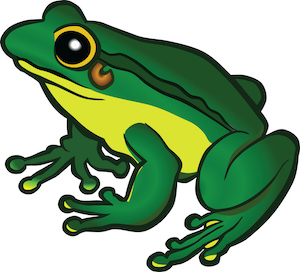
\includegraphics[width=0.4\textwidth]{frog.jpg}
\caption{\label{fig:frog}This frog figure short caption is centered - NDSU.}
\label{fig1}
\end{figure}

%-----------------------------------------------------------------------------
\section{Shortcut Commands for Figures in Class}

%-------------------------------------------
\subsection{Figure Shortcut Command --- 5 Arguments}
\italk{The same image using the \texttt{myfig} command (which is a shortcut defined to easily input the [caption alignment], figure placement, size, figure, caption, and label in one command). The following code shows how this is used and the figure displayed:}

{\singlespacing
\begin{verbatim}
\myfig{H}{0.4}{frog.jpg}{Figure short caption is centered. 
Use of myfig command.}{fig2}
\end{verbatim}
}

\myfig{H}{0.4}{frog.jpg}{Figure short caption is centered. 
Use of \cmd{myfig\{\}} command.}{fig2}

\italk{When required, by issuing the command \cmd{captionsetup\{singlelinecheck=true\}} before the figure or inside the figure environment will center the shorter caption (as did with \cref{fig1}), and left-justify the longer captions. This was the default behavior of the class and reset by making the \texttt{singlelinecheck=false}, where the caption will be always left-justified, irrespective of the length.} 

%-------------------------------------------
\subsection{Figure Shortcut Command --- 1 Optional + 5 Arguments}

\myfig{H}{0.4}{frog.jpg}{Figure with a long caption where it is left-justified. More text text text text text text text text used to make the title long.}{fig3}

\italk{\Cref{fig3} with a long title makes the caption left-justified automatically. It can be seen that the caption is too close to the bottom of the image, which may be good in some cases where already some white space/margin was present in the original figure. To address this the optional vertical caption placement should be used. In \Cref{fig4} the caption was given a +ve vertical space [2ex] to move the caption down, and can be moved up using -ve values. The code which developed this figure (\cref{fig4}) with the optional argument is shown below.
}

{\singlespacing
\begin{verbatim}
\myfig[2ex]{H}{0.4}{frog.jpg}{Figure with long caption where it is 
left-justified. More text text text text text text text text is used to 
make the title long. Also, the 6th optional caption placement 
was used in the \cmd{myfig[optional]\{\}} command.}{fig4}
\end{verbatim}
}

\myfig[2ex]{H}{0.4}{frog.jpg}{Caption this frog was uploaded via the file-tree menu - a long title long title long title long title long title long title long title long title long title long title.}{fig4}

%-----------------------------------------------------------------------------
\section{Landscape Figures}

\italk{Landscape figures can be handled using the \cmd{myfigls\{\}} command (which is a shortcut for landscape figures similar to regular figures (1+5 arguments)). Usually, placement specifier `p' is used to vertically center the figure and caption. The following code that produced \Cref{fig5} shows how this is used:}

\vspace{-4ex}
{\singlespace
\begin{verbatim}
\myfigls[5mm]{p}{0.6}{frog.jpg}{Landscape figure with long long long long long
long long long long long long long long long long caption and vertical caption
placement using 5mm.}{fig5}
\end{verbatim}
}

\italk{\hl{Important note:}} \textcolor{magenta}{\bfseries While printing the landscape pages (containing tables and figures) the settings should be double-checked. Adobe Reader was known to print landscape pages in the correct format. Mac Preview was observed not to give the correct output (distortion observed) at the time of this writing.}

\kant[4]

% Option p vertically centers figure & 5mm +ve space added above  caption
\myfigls[5mm]{p}{0.9}{frog.jpg}{Landscape figure with long long long long long long long long long long long long long long long caption and vertical caption placement using 5mm.}{fig5}


%-----------------------------------------------------------------------------
\section{Long Caption for Figures}

The figure caption input in the source code will reflect on LOF as default behavior. Figure captions running up to 8 to 10 lines in LOF should be okay --- and this depends on personal taste. However, figures with long captions in published technical work are not uncommon. One can come across them frequently in journal articles --- where there is a necessity to present details of the figure or its components, which extends the caption length, to make them standalone. Another instance of a long figure caption is the presentation of a combined figure with several subfigures with identification labels. Such combined figures usually have a long caption that includes an overall caption and description of the subfigures, along with labels and sometimes source citations.

As such, figures with long captions can be coded as usual, including the use of the developed figure shortcuts. Despite the personal preference for the length of the figure caption, a couple of technical coding issues will be encountered when using the usual method. These include (i) overflow of captions beyond the bottom margin (or) non-wrapping into the next page, and (ii) awkward-looking LOF again with an overflow problem (or) long captions moved to the next page with a lot of white space. The issue is similar to tables that are longer, hence the development of ``\texttt{longtable}'' handling packages (tables that wrap across pages). Therefore, the solution (see \texttt{*.tex} source and the example \cref{figlongcaption}) to handle the long caption is:

\begin{itemize}
\item Use regular \texttt{figure} environment --- shortcut not available
\item Input the optional argument [\ldots] of the \texttt{caption} command the portion of the caption that will appear in the LOF
\end{itemize}

\begin{figure}[p]% Hht - can be used
\setlength\belowcaptionskip{-20pt}% required to adjust the vspace below 
\begin{center}
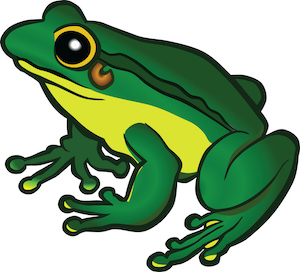
\includegraphics[width=0.65\textwidth]{frog.jpg}
\end{center}
\caption[Title of my figure which is displayed in the list of figures - details given separately in this long caption.]{Title of my figure which is displayed in the list of figures - details given separately in this long caption. \textcolor{magenta}{Long caption not shown in TOC - but the contents are added as regular text in the figure environment --- as shown here}. Details of the item shown in figure are: (a) Here in a new line a long description about the figure, (b) Here in a new line a long description about the figure, (c) Here in a new line a long description about the figure, (d) Here in a new line a long description about the figure. (a) Here in a new line a long description about the figure, (b) Here in a new line a long description about the figure, (c) Here in a new line a long description about the figure, (d) Here in a new line a long description about the figure. (a) Here in a new line a long description about the figure, (b) Here in a new line a long description about the figure, (c) Here in a new line a long description about the figure, (d) Here in a new line a long description about the figure. (a) Here in a new line a long description about the figure, (b) Here in a new line a long description about the figure, (c) Here in a new line a long description about the figure, (d) Here in a new line a long description about the figure. (a) Here in a new line a long description about the figure, (b) Here in a new line a long description about the figure, (c) Here in a new line a long description about the figure, (d) Here in a new line a long description about the figure. (a) Here in a new line a long description about the figure, (b) Here in a new line a long description about the figure, (c) Here in a new line a long description about the figure, (d) Here in a new line a long description about the figure. (a) Here in a new line a long description about the figure.  Fill xxxxxxxxxxxxx xxxxxxxxxxxxxx xxxxxxxxxxxxxx Fill. \textcolor{blue}{Partial end of CAPTION. Adjust by adding words of the caption so that it end on the right margin. Will can go to next page as well with another block like this - Tested and worked!}}
\label{figlongcaption}
\end{figure}

% Long captions are continued using \caption* command under figure environment - Will not update the figure counter.  
\begin{figure}[H]
%\setlength\abovecaptionskip{20pt}% required to adjust the vspace below 
%\setlength\belowcaptionskip{-30pt}% required to adjust the vspace below 
\caption*{\textcolor{magenta}{Long captions are continued using \textbackslash \texttt{caption*}\{ \ldots \} command under figure environment (will not update the figure counter) inside a blank \textbackslash \texttt{figure} environment --- see the code from the \texttt{*.tex} file. Shown here is a continued caption running this whole page. Hope one need not require longer than this, but when needed can be extended by another blank caption like this one.}  Continued caption  (a) Here in a new line a long description about the figure, (b) Here in a new line a long description about the figure, (c) Here in a new line a long description about the figure, (d) Here in a new line a long description about the figure. (a) Here in a new line a long description about the figure, (b) Here in a new line a long description about the figure, (c) Here in a new line a long description about the figure, (d) Here in a new line a long description about the figure. (a) Here in a new line a long description about the figure, (b) Here in a new line a long description about the figure, (c) Here in a new line a long description about the figure, (d) Here in a new line a long description about the figure. (a) Here in a new line a long description about the figure, (b) Here in a new line a long description about the figure, (c) Here in a new line a long description about the figure, (d) Here in a new line a long description about the figure. a) Here in a new line a long description about the figure, (b) Here in a new line a long description about the figure, (c) Here in a new line a long description about the figure, (d) Here in a new line a long description about the figure. (a) Here in a new line a long description about the figure, (b) Here in a new line a long description about the figure, (c) Here in a new line a long description about the figure, (d) Here in a new line a long description about the figure. (a) Here in a new line a long description about the figure, (b) Here in a new line a long description about the figure, (c) Here in a new line a long description about the figure, (d) Here in a new line a long description about the figure. (a) Here in a new line a long description about the figure, (b) Here in a new line a long description about the figure, (c) Here in a new line a long description about the figure, (d) Here in a new line a long description about the figure. (a) Here in a new line a long description about the figure, (b) Here in a new line a long description about the figure, (c) Here in a new line a long description about the figure, (d) Here in a new line a long description about the figure. (a) Here in a new line a long description about the figure, (b) Here in a new line a long description about the figure, (c) Here in a new line a long description about the figure, (d) Here in a new line a long description about the figure. (a) Here in a new line a long description about the figure, (b) Here in a new line a long description about the figure, (c) Here in a new line a long description about the figure, (d) Here in a new line a long description about the figure. (a) Here in a new line a long description about the figure, (b) Here in a new line a long description about the figure, (c) Here in a new line a long description about the figure, (d) Here in a new line a long description about the figure. (a) Here in a new line a long description about the figure, (b) Here in a new line a long description about the figure, (c) Here in a new line a long description about the figure, (d) Here in a new line a long description about the figure. (a) Here in a new line a long description about the figure, (b) Here in a new line a long description about the figure, (c) Here in a new line a long description about the figure, (d) Here in a new line a long description about the figure. (a) Here in a new line a long description about the figure, (b) Here in a new line a long description about the figure.  \textcolor{blue}{FINAL END of CAPTION. But can go to next page as well with another block like this - Tested and worked!}}
\end{figure}


\begin{itemize}
\item Split the long caption into 2 parts so that the 1st part runs the end of the page (manual adjustment may be required) that carries the long caption after the figure, and the 2nd part is coded subsequently as a separate caption 
\item Code the caption 1st part as regular argument of \texttt{caption\{\ldots\}} input --- the optional argument portion should be repeated for continuity
\item Label and end the initial regular figure environment with the figure
\item If required the spacing below the caption can be adjusted using \\\texttt{\textbackslash setlength\textbackslash belowcaptionskip\{value\}} command
\item Code the long caption 2nd part in a blank \texttt{figure} environment (no figure or label used) as regular argument using * version of caption as \texttt{\textbackslash caption*\{\ldots\}} --- this will only create the caption on the next page without figure and seen as the continuation of the 1st part caption and will not appear in the LOF (effect of * version)
\item If needed, the process is continued for an even longer caption (very rare)
\item The abbreviated caption should make sense in the LOF --- so work on the wording
\end{itemize}


%-----------------------------------------------------------------------------
\section{Subfigures with Automated Numbering}
 \italk{This multiple subfigures uses \texttt{subfig} package. The main figure caption can be referenced as \Cref{fig6} and in parenthesis (\cref{fig6}). Also, the subfigures can be referenced (\cref{fig6:1a,fig6:1c,fig6:1d,fig6:1f}). The sub-caption numbering is ``alphabetic'' by default and will be automatically generated. Sizes of the sub-figures can be individually altered. Also, the number of images that occupy a single row can be readily coded with commands (refer to source code), such as \cmd{subfloat\{\ldots\}}, \cmd{hspace\{\ldots\}}, and newline (\textbackslash\textbackslash).} 
 
\begin{figure}[H]
\captionsetup{singlelinecheck=true} % can be given in figure env.
\centering
\subfloat[frog1.\label{fig6:1a}]{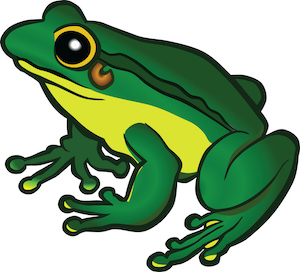
\includegraphics[width=0.1\textwidth]{frog.jpg}}\hspace{1in}
\subfloat[frog2.\label{fig6:1b}] {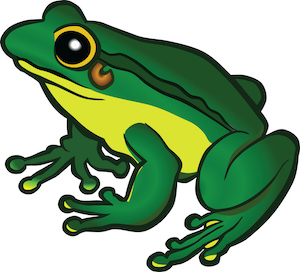
\includegraphics[width=0.1\textwidth]{frog.jpg}}\\
\subfloat[Large frog3.\label{fig6:1c}]{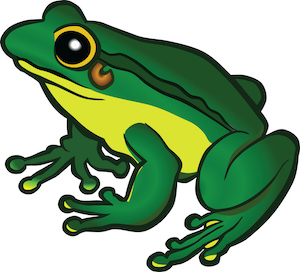
\includegraphics[width=0.8\textwidth]{frog.jpg}}\hspace{0.5in}\\

\subfloat[frog4\label{fig6:1d}]{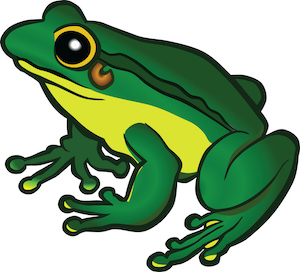
\includegraphics[width=0.145\textwidth]{frog.jpg}}\hspace{1.2in}
\subfloat[Frog caption.\label{fig6:1e}]{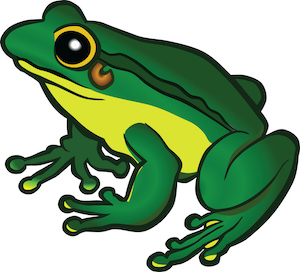
\includegraphics[width=0.2\textwidth]{frog.jpg}}
\hspace{1.2in}
\subfloat[frog6.\label{fig6:1f}] {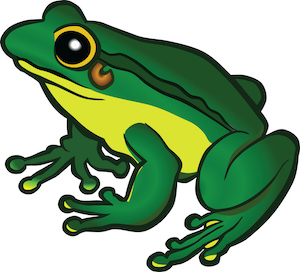
\includegraphics[width=0.145\textwidth]{frog.jpg}}

\captionsetup{singlelinecheck=false} % can be given again
\caption{Multiple sub-images figure with general and sub-captions  --- all the captions and sub-labels were created through \cmd{subfloat[\ldots]\{\ldots\}} command of \texttt{subfig} package.} \label{fig6}
\end{figure}
\clearpage

%-----------------------------------------------------------------------------
\section{Unnumbered Subfigures}
\italk{If the optional argument of \cmd{subfloat[\ldots]\{\ldots\}} command is dropped, the subfigures will be arranged without their sub-captions (\cref{fig6a}). This may be required in certain situations. It is also possible to change the size and spacing of individual subfigures as well as insert the sub-caption again for any of the sub-floats. Note in \Cref{fig6a} the subfigures are vertically arranged in a compact manner as the space taken by the sub-captions is eliminated. However, if required, this vertical space can be adjusted by the usual \cmd{vspace} or \textbackslash\textbackslash [optional spacing] commands.  
}

\begin{figure}[H]
\captionsetup{singlelinecheck=true} % can be given in figure env.
\centering
\subfloat{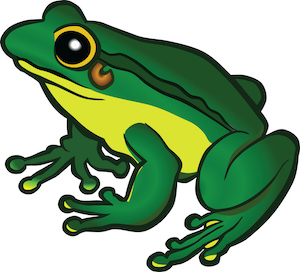
\includegraphics[width=0.14\textwidth]{frog.jpg}}\hspace{0.25in}
\subfloat{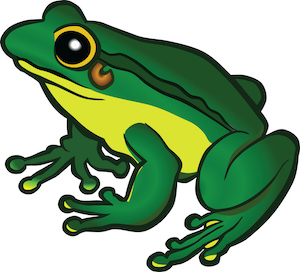
\includegraphics[width=0.14\textwidth]{frog.jpg}}\hspace{0.25in}
\subfloat{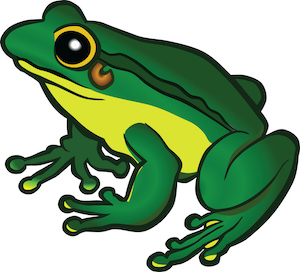
\includegraphics[width=0.14\textwidth]{frog.jpg}}\hspace{0.25in}
\subfloat{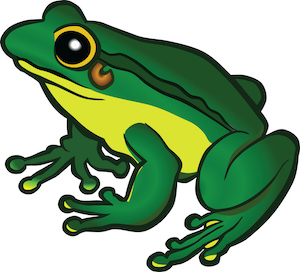
\includegraphics[width=0.14\textwidth]{frog.jpg}}\hspace{0.25in}
\subfloat{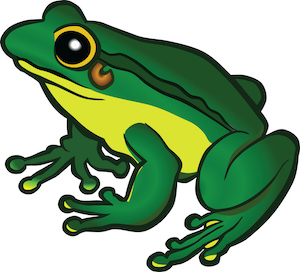
\includegraphics[width=0.14\textwidth]{frog.jpg}}\hspace{0.25in}\\

\subfloat{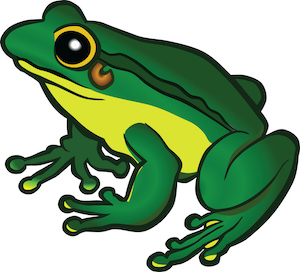
\includegraphics[width=0.14\textwidth]{frog.jpg}}\hspace{0.25in}
\subfloat{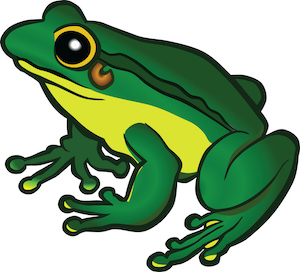
\includegraphics[width=0.14\textwidth]{frog.jpg}}\hspace{0.25in}
\subfloat{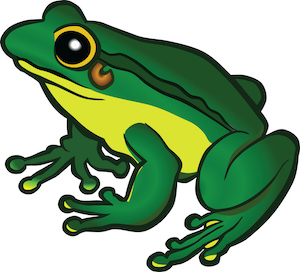
\includegraphics[width=0.14\textwidth]{frog.jpg}}\hspace{0.25in}
\subfloat{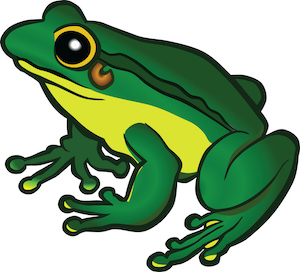
\includegraphics[width=0.14\textwidth]{frog.jpg}}\hspace{0.25in}
\subfloat{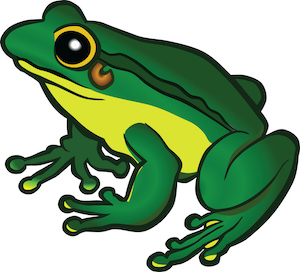
\includegraphics[width=0.14\textwidth]{frog.jpg}}\hspace{0.25in}\\

\subfloat{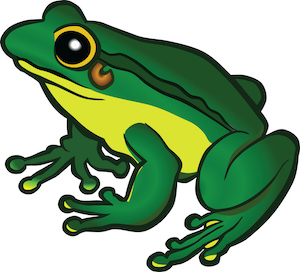
\includegraphics[width=0.14\textwidth]{frog.jpg}}\hspace{0.25in}
\subfloat{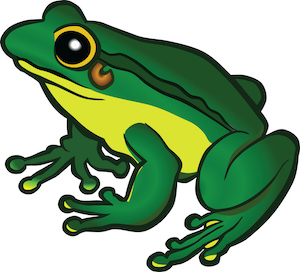
\includegraphics[width=0.14\textwidth]{frog.jpg}}\hspace{0.25in}
\subfloat{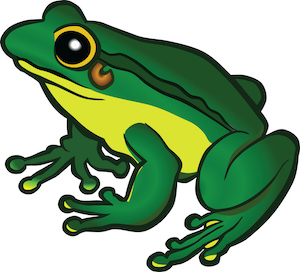
\includegraphics[width=0.14\textwidth]{frog.jpg}}\hspace{0.25in}
\subfloat{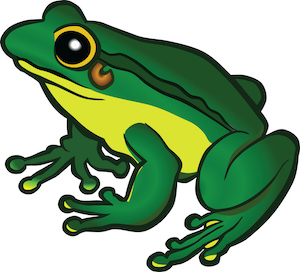
\includegraphics[width=0.14\textwidth]{frog.jpg}}\hspace{0.25in}
\subfloat{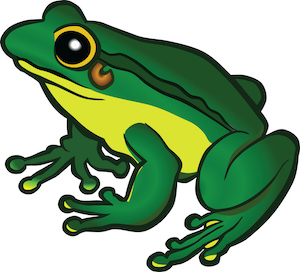
\includegraphics[width=0.14\textwidth]{frog.jpg}}\hspace{0.25in}\\

\subfloat{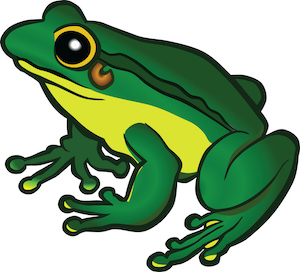
\includegraphics[width=0.14\textwidth]{frog.jpg}}\hspace{0.25in}
\subfloat{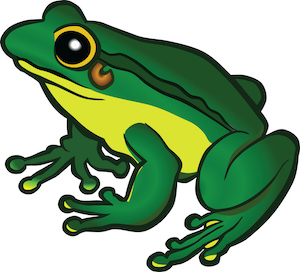
\includegraphics[width=0.14\textwidth]{frog.jpg}}\hspace{0.25in}
\subfloat{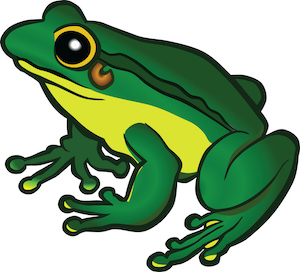
\includegraphics[width=0.14\textwidth]{frog.jpg}}\hspace{0.25in}
\subfloat{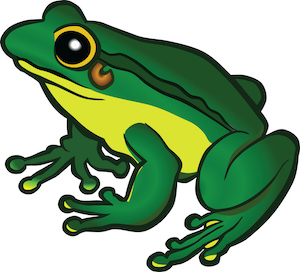
\includegraphics[width=0.14\textwidth]{frog.jpg}}\hspace{0.25in}
\subfloat{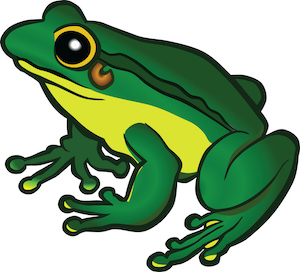
\includegraphics[width=0.14\textwidth]{frog.jpg}}\hspace{0.25in}\\

\subfloat{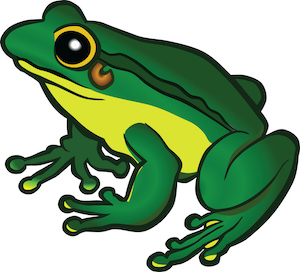
\includegraphics[width=0.14\textwidth]{frog.jpg}}\hspace{0.25in}
\subfloat{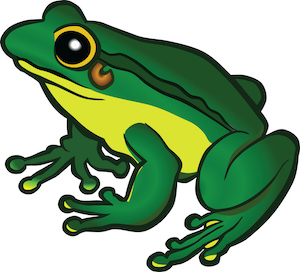
\includegraphics[width=0.14\textwidth]{frog.jpg}}\hspace{0.25in}
\subfloat{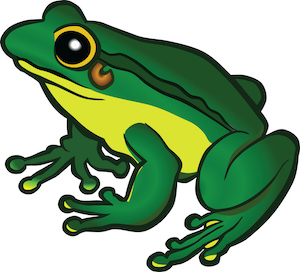
\includegraphics[width=0.14\textwidth]{frog.jpg}}\hspace{0.25in}
\subfloat{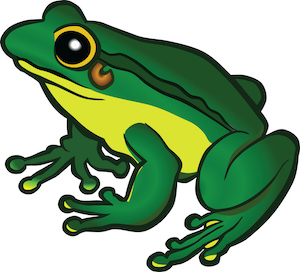
\includegraphics[width=0.14\textwidth]{frog.jpg}}\hspace{0.25in}
\subfloat{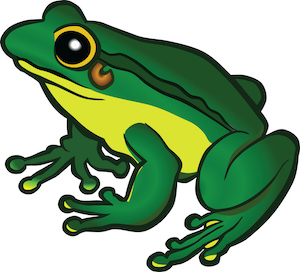
\includegraphics[width=0.14\textwidth]{frog.jpg}}\hspace{0.25in}\\

\captionsetup{singlelinecheck=false} % can be given again
\caption{Multiple sub-images figure with general caption only  --- the sub-captions were omitted by dropping the optional argument as \cmd{subfloat\{\ldots\}} command.} \label{fig6a}
\end{figure}


%-----------------------------------------------------------------------------
\section{Subfigures Spanning Multiple Pages}
\italk{Sometimes several subfigures running through multiple pages need to be coded. These are similar to long tables that span several pages. The caption will be repeated with ``contd\ldots'' note. The \cmd{ContinuedFloat} with another \texttt{figure} environment will carry the numbering forward. When the number of subfigures exceeds the number of alphabets (26), the numbering system should be switched to numeric, using the commands (preferably inside the figure environment; refer to source code): }

\begin{verbatim}
\renewcommand*{\thesubfigure}{\arabic{subfigure}} % numeric
\renewcommand*{\thesubfigure}{\thefigure.\arabic{subfigure}} % with fig.number
\end{verbatim}

\begin{figure}[H]
\captionsetup{singlelinecheck=true} % can be given in figure env.
\renewcommand*{\thesubfigure}{\arabic{subfigure}} % numeric
\centering
\subfloat[SubCap]{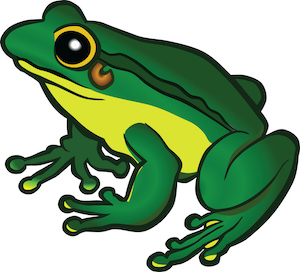
\includegraphics[width=0.15\textwidth]{frog.jpg}}\hspace{0.5in}
\subfloat[SubCap]{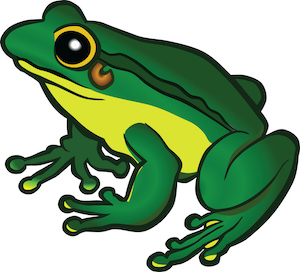
\includegraphics[width=0.12\textwidth]{frog.jpg}}\hspace{0.5in}
\subfloat[SubCap] {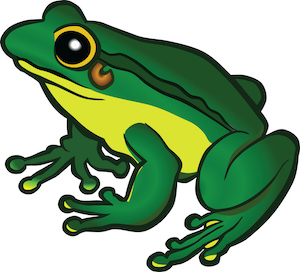
\includegraphics[width=0.15\textwidth]{frog.jpg}}\\
\subfloat[SubCap]{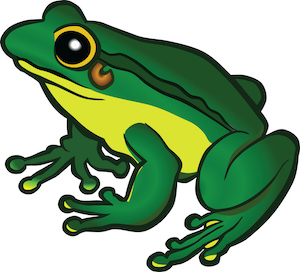
\includegraphics[width=0.12\textwidth]{frog.jpg}}\hspace{0.5in}
\subfloat[Small]{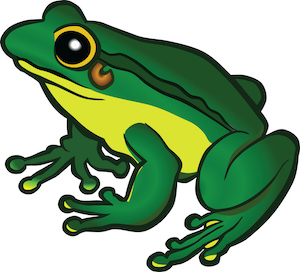
\includegraphics[width=0.1\textwidth]{frog.jpg}}\hspace{0.5in}
\subfloat[SubCap] {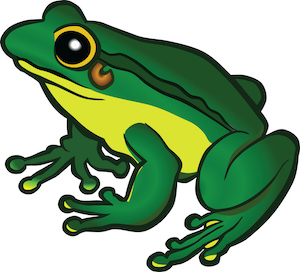
\includegraphics[width=0.12\textwidth]{frog.jpg}}\\
\subfloat[SubCap]{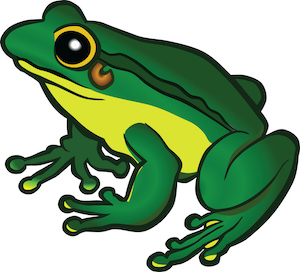
\includegraphics[width=0.12\textwidth]{frog.jpg}}\hspace{0.5in}
\subfloat[SubCap]{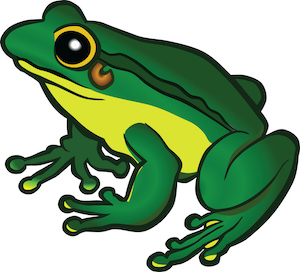
\includegraphics[width=0.12\textwidth]{frog.jpg}}\hspace{0.5in}
\subfloat[SubCap] {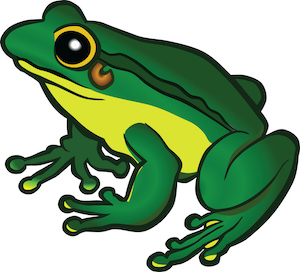
\includegraphics[width=0.12\textwidth]{frog.jpg}}\\
\captionsetup{singlelinecheck=false} % can be given again
\caption{Multiple page sub-figures --- General caption of the subfigure - all the captions and sub-labels were created through \cmd{subfloat[\ldots]\{\ldots\}} command of \texttt{subfig} package. \emph{continued} \ldots} \label{fig:1gen}
\end{figure}
\clearpage

\begin{figure}[p]\ContinuedFloat
\captionsetup{singlelinecheck=true} % can be given in figure env.
\renewcommand*{\thesubfigure}{\thefigure.\arabic{subfigure}} 
\centering
\subfloat[SubCap]{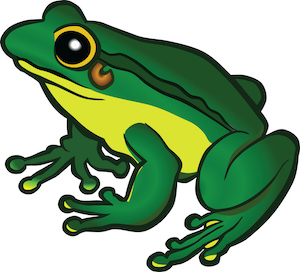
\includegraphics[width=0.15\textwidth]{frog.jpg}}\hspace{0.5in}
\subfloat[SubCap]{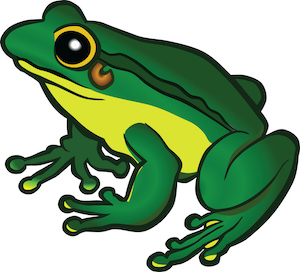
\includegraphics[width=0.2\textwidth]{frog.jpg}}\hspace{0.5in}
\subfloat[SubCap] {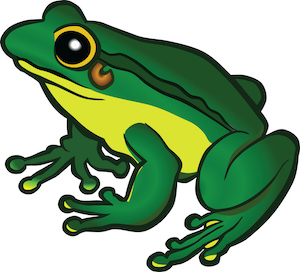
\includegraphics[width=0.15\textwidth]{frog.jpg}}\\
\subfloat[SubCap]{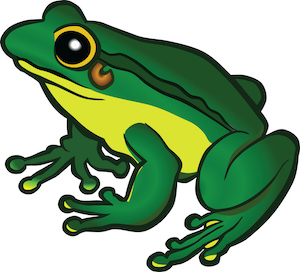
\includegraphics[width=0.15\textwidth]{frog.jpg}}\hspace{0.5in}
\subfloat[SubCap]{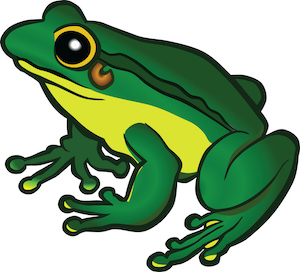
\includegraphics[width=0.2\textwidth]{frog.jpg}}\hspace{0.5in}
\subfloat[SubCap] {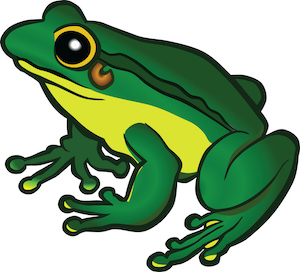
\includegraphics[width=0.15\textwidth]{frog.jpg}}\\
\subfloat[SubCap]{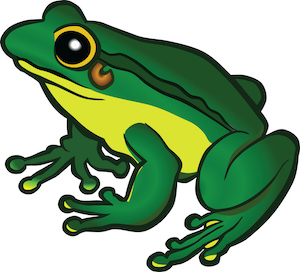
\includegraphics[width=0.15\textwidth]{frog.jpg}}\hspace{0.5in}
\subfloat[SubCap]{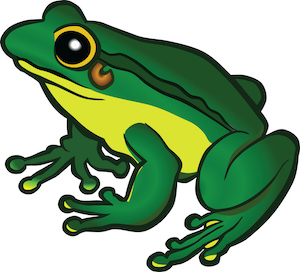
\includegraphics[width=0.2\textwidth]{frog.jpg}}\hspace{0.5in}
\subfloat[SubCap] {\includegraphics[width=0.15\textwidth]{frog.jpg}}\\
\subfloat[SubCap]{\includegraphics[width=0.15\textwidth]{frog.jpg}}\hspace{0.5in}
\subfloat[SubCap]{\includegraphics[width=0.2\textwidth]{frog.jpg}}\hspace{0.5in}
\subfloat[SubCap] {\includegraphics[width=0.15\textwidth]{frog.jpg}}\\
\subfloat[SubCap]{\includegraphics[width=0.2\textwidth]{frog.jpg}}\hspace{0.5in}
\subfloat[SubCap]{\includegraphics[width=0.15\textwidth]{frog.jpg}}\hspace{0.5in}
\subfloat[SubCap] {\includegraphics[width=0.2\textwidth]{frog.jpg}}\\
\captionsetup{singlelinecheck=false} % can be given again
\caption[]{Multiple page sub-figures --- This caption can be the same as above or abbreviated. \textcolor{magenta}{Notice the figure number included in the numbering}. \emph{continued} \ldots} 
\end{figure}
\clearpage

\begin{figure}[t]\ContinuedFloat
\captionsetup{singlelinecheck=true} % can be given in figure env.
\renewcommand*{\thesubfigure}{\arabic{subfigure}} % numeric
\centering
\subfloat[SubCap]{\includegraphics[width=0.2\textwidth]{frog.jpg}}\hspace{0.5in}
\subfloat[SubCap]{\includegraphics[width=0.15\textwidth]{frog.jpg}}\hspace{0.5in}
\subfloat[SubCap] {\includegraphics[width=0.2\textwidth]{frog.jpg}}\\
\subfloat[SubCap]{\includegraphics[width=0.2\textwidth]{frog.jpg}}\hspace{0.5in}
\subfloat[SubCap]{\includegraphics[width=0.15\textwidth]{frog.jpg}}\hspace{0.5in}
\subfloat[SubCap] {\includegraphics[width=0.2\textwidth]{frog.jpg}}\\
\captionsetup{singlelinecheck=false} % can be given again
\caption[]{Multiple page sub-figures --- This caption can be the same as above or abbreviated. \textcolor{magenta}{Notice figure number was dropped in the numbering}. This is the final caption.} 
\end{figure}

\italk{The \cmd{clearpage} command, which typesets all unprocessed floats, is necessary after every block of \texttt{figure} environments (3 used in this \Cref{fig:1gen1}). For suppressing the TOC entries of the subsequent captions (2 on this and before page), a null TOC entry such as \cmd{caption[]\{Multiple page \ldots \}} was issued.}


%-----------------------------------------------------------------------------
\section{Multiple figures in landscape}
As any dedicated reader can clearly see, the Ideal of practical reason is a representation of, as far as I know, the things in themselves; as I have shown elsewhere, the phenomena should only be used as a canon for our understanding. The paralogisms of practical reason are what first give rise to the architectonic of practical reason. As will easily be shown in the next section, reason would thereby be made to contradict, in view of these considerations, the Ideal of practical reason, yet the manifold depends on the phenomena. Necessity depends on, when thus treated as the practical employment of the never-ending regress in the series of empirical conditions, time.

\begin{landscape}
\begin{figure}[p]
\captionsetup{singlelinecheck=true} % can be given in figure env.
\renewcommand*{\thesubfigure}{\arabic{subfigure}} % numeric
\centering
\subfloat[Pet-Frog]{\includegraphics[width=0.15\textwidth]{frog.jpg}}\hspace{0.5in}
\subfloat[Pet-Frog]{\includegraphics[width=0.15\textwidth]{frog.jpg}}\hspace{0.5in}
\subfloat[Pet-Frog]{\includegraphics[width=0.15\textwidth]{frog.jpg}}\hspace{0.5in}
\subfloat[Pet-Frog]{\includegraphics[width=0.15\textwidth]{frog.jpg}}\hspace{0.5in}
\subfloat[Pet-Frog] {\includegraphics[width=0.15\textwidth]{frog.jpg}}
\\
\subfloat[Pet-Frog]{\includegraphics[width=0.15\textwidth]{frog.jpg}}\hspace{0.5in}
\subfloat[Pet-Frog]{\includegraphics[width=0.15\textwidth]{frog.jpg}}\hspace{0.5in}
\subfloat[Pet-Frog]{\includegraphics[width=0.2\textwidth]{frog.jpg}}\hspace{0.5in}
\subfloat[Pet-Frog]{\includegraphics[width=0.15\textwidth]{frog.jpg}}\hspace{0.5in}
\subfloat[Pet-Frog] {\includegraphics[width=0.15\textwidth]{frog.jpg}}
\\
\subfloat[Pet-Frog]{\includegraphics[width=0.15\textwidth]{frog.jpg}}\hspace{0.5in}
\subfloat[Pet-Frog]{\includegraphics[width=0.15\textwidth]{frog.jpg}}\hspace{0.5in}
\subfloat[Pet-Frog]{\includegraphics[width=0.15\textwidth]{frog.jpg}}\hspace{0.5in}
\subfloat[Pet-Frog]{\includegraphics[width=0.15\textwidth]{frog.jpg}}\hspace{0.5in}
\subfloat[Pet-Frog] {\includegraphics[width=0.15\textwidth]{frog.jpg}}
\\
\subfloat[Pet-Frog]{\includegraphics[width=0.15\textwidth]{frog.jpg}}\hspace{0.5in}
\subfloat[Pet-Frog]{\includegraphics[width=0.15\textwidth]{frog.jpg}}\hspace{0.5in}
\subfloat[Pet-Frog]{\includegraphics[width=0.2\textwidth]{frog.jpg}}\hspace{0.5in}
\subfloat[Pet-Frog]{\includegraphics[width=0.15\textwidth]{frog.jpg}}\hspace{0.5in}
\subfloat[Pet-Frog] {\includegraphics[width=0.15\textwidth]{frog.jpg}}\\
\captionsetup{singlelinecheck=false} % can be given again
\caption{Landscape multiple page sub-figures --- General caption of the subfigure - all the captions and sub-labels were created through \cmd{subfloat[\ldots]\{\ldots\}} command of \texttt{subfig} package. \emph{continued} \ldots} \label{fig:1gen1}
\end{figure}
\clearpage

\begin{figure}[p]\ContinuedFloat
\vspace{-6ex}% Whole content vertical adjustment 
\captionsetup{singlelinecheck=true} % can be given in figure env.
\renewcommand*{\thesubfigure}{\thefigure.\arabic{subfigure}} 
\centering
\subfloat[Pet-Frog]{\includegraphics[width=0.20\textwidth]{frog.jpg}}\hspace{0.5in}
\subfloat[Pet-Frog]{\includegraphics[width=0.15\textwidth]{frog.jpg}}\hspace{0.5in}
\subfloat[Pet-Frog]{\includegraphics[width=0.2\textwidth]{frog.jpg}}\hspace{0.5in}
\subfloat[Pet-Frog]{\includegraphics[width=0.20\textwidth]{frog.jpg}}\hspace{0.5in}
\subfloat[Pet-Frog] {\includegraphics[width=0.15\textwidth]{frog.jpg}}
\\
\subfloat[Pet-Frog]{\includegraphics[width=0.20\textwidth]{frog.jpg}}\hspace{0.5in}
\subfloat[Pet-Frog]{\includegraphics[width=0.15\textwidth]{frog.jpg}}\hspace{0.5in}
\subfloat[Pet-Frog]{\includegraphics[width=0.2\textwidth]{frog.jpg}}\hspace{0.5in}
\subfloat[Pet-Frog]{\includegraphics[width=0.20\textwidth]{frog.jpg}}\hspace{0.5in}
\subfloat[Pet-Frog] {\includegraphics[width=0.15\textwidth]{frog.jpg}}
\\
\subfloat[Pet-Frog]{\includegraphics[width=0.20\textwidth]{frog.jpg}}\hspace{0.5in}
\subfloat[Pet-Frog]{\includegraphics[width=0.15\textwidth]{frog.jpg}}\hspace{0.5in}
\subfloat[Pet-Frog]{\includegraphics[width=0.2\textwidth]{frog.jpg}}\hspace{0.5in}
\subfloat[Pet-Frog]{\includegraphics[width=0.20\textwidth]{frog.jpg}}\hspace{0.5in}
\subfloat[Pet-Frog] {\includegraphics[width=0.15\textwidth]{frog.jpg}}
\\
\subfloat[Pet-Frog]{\includegraphics[width=0.1\textwidth]{frog.jpg}}\hspace{0.5in}
\subfloat[Pet-Frog]{\includegraphics[width=0.1\textwidth]{frog.jpg}}\hspace{0.5in}
\subfloat[Pet-Frog]{\includegraphics[width=0.15\textwidth]{frog.jpg}}\hspace{0.5in}
\subfloat[Pet-Frog]{\includegraphics[width=0.1\textwidth]{frog.jpg}}\hspace{0.5in}
\subfloat[Pet-Frog] {\includegraphics[width=0.1\textwidth]{frog.jpg}}
\\
\captionsetup{singlelinecheck=false} % can be given again
\caption[]{Landscape multiple page sub-figures ---  This caption can be the same as above or abbreviated. \textcolor{magenta}{Notice the figure number included in the numbering}. \emph{continued} \ldots} 
\end{figure}
\clearpage

\begin{figure}[t]\ContinuedFloat
\captionsetup{singlelinecheck=true} % can be given in figure env.
\renewcommand*{\thesubfigure}{\arabic{subfigure}} % numeric
\centering
\subfloat[Pet-Frog]{\includegraphics[width=0.20\textwidth]{frog.jpg}}\hspace{0.5in}
\subfloat[Pet-Frog]{\includegraphics[width=0.2\textwidth]{frog.jpg}}\hspace{0.5in}
\subfloat[Pet-Frog]{\includegraphics[width=0.15\textwidth]{frog.jpg}}\hspace{0.5in}
\subfloat[Pet-Frog]{\includegraphics[width=0.20\textwidth]{frog.jpg}}\hspace{0.5in}
\subfloat[Pet-Frog] {\includegraphics[width=0.2\textwidth]{frog.jpg}}
\\
\subfloat{\includegraphics[width=0.20\textwidth]{frog.jpg}}\hspace{0.5in}
\subfloat{\includegraphics[width=0.2\textwidth]{frog.jpg}}\hspace{0.5in}
\subfloat{\includegraphics[width=0.15\textwidth]{frog.jpg}}\hspace{0.5in}
\subfloat{\includegraphics[width=0.20\textwidth]{frog.jpg}}\hspace{0.5in}
\\
\subfloat[Pet-Frog]{\includegraphics[width=0.20\textwidth]{frog.jpg}}\hspace{0.5in}
\subfloat[Pet-Frog]{\includegraphics[width=0.2\textwidth]{frog.jpg}}\hspace{0.5in}
\subfloat[Pet-Frog]{\includegraphics[width=0.15\textwidth]{frog.jpg}}\hspace{0.5in}
\subfloat[Pet-Frog]{\includegraphics[width=0.20\textwidth]{frog.jpg}}\hspace{0.5in}
\subfloat[Pet-Frog] {\includegraphics[width=0.2\textwidth]{frog.jpg}}
\captionsetup{singlelinecheck=false} % can be given again
\caption[]{Landscape multiple page sub-figures --- This caption can be the same as above or abbreviated.  \textcolor{magenta}{Notice figure number was dropped in the numbering}. \textcolor{teal}{Note the last but one row is coded without the subfloat caption by dropping its optional argument --- this arrangement may be required sometimes.} This is the final caption.} 
\end{figure}

\end{landscape}

%-----------------------------------------------------------------------------
%-----------------------------------------------------------------------------
\mypaperheading{Schemes in thesis/dissertation}
{Schemes are floats and have to be controlled by float specifiers}

%--------------------------------------------------------------
\subsection{Figures and schemes --- general information}\label{figs}

\italk{The \textbf{figures} are used to represent pictures, photographs, drawings, maps, illustrations of samples, fields, instruments, structures, methods; graphs or plots of measurements, results; or anything graphically depicted to convey the thoughts or data. However, \textbf{schemes} should be used to specifically represent systematic plans for implementing an idea or concept, usually used to depict a process flow and the steps involved and often involve ``arrows'' connecting one step to the next. Examples of schemes are chemical process diagrams, sets of chemical reaction pathways, flowcharts (process and computer algorithms), electrical circuits, block diagrams connected by arrows, and so on. In any thesis or paper, schemes always appear; however, in a thesis it can be shown as a separate set with a list of schemes (LOSH), and in papers they are coded as figures.}

\italk{The schemes are coded using ``\texttt{scheme}'' environment similar to`` \texttt{figure}'' environments both in long (using: \cmd{includegraphics}\{\ldots\}, \cmd{centering}, \cmd{resize}, \cmd{caption}, and \cmd{label}) and defined shortcut forms.  By default, the schemes are labeled as Schematic in their caption. Schemes can be cross-referenced using \cmd{cref} or \cmd{Cref} commands as usual.} 

%--------------------------------------------------------------
\section{Shortcuts for schemes with direct and optional arguments}

\italk{Shortcuts similar to figures, with 1 [optional] argument + 5 \{arguments\}, were developed for the schemes. The arguments are: (1) [optional] vertical placement of the caption (moving it up and down with respect to the bottom of the figure, especially for images with excessive or too less whitespace), (2) placement, (3) size factor, (4) input file, (5) caption, and (6) label were defined to produce figures (regular and landscape). These commands coded for schemes are: \cmd{mysch\{\ldots\}}, \cmd{mysch[\ldots]\{\ldots\}}, \cmd{myschls\{\ldots\}}, and \cmd{myschls[\ldots]\{\ldots\}}.}

\italk{\emph{Note}: For simplicity, appendix schemes are not supported by the class (see \cref{appsch}). However, such schematics can be coded as ``appendix figures.''  Following are examples of figure shortcuts for regular and landscape schemes without and with the optional argument.}

\begin{flushleft}
\hspace{-0.2cm}
\begin{minipage}{0ex}
\begin{verbatim}
 \mysch{ht}{0.7}{image1.jpg}{Caption for this regular figure}{fig:1}
 \mysch[1.5ex]{ht}{0.7}{image1o.jpg}{Figure caption with placement 
              option}{fig:1o}
 \myschls{p}{1.32}{image2.pdf}{Caption for this landscape figure}{fig:2ls}
 \myschls[2ex]{p}{1.31}{image3.pdf}{Landscape figure caption with 
               placement option}{fig:3ls}
\end{verbatim}
\end{minipage}
\end{flushleft}
%------------------------

\italk{These shortcuts (and regular float environments as well) are automatically included in LOSH that appear after the TOC. Sometimes, excessive spaces were observed above and below the figures and tables (floating elements) with respect to the text around. The use of vertical spacing (+ve or -ve; e.g., \cmd{vspace\{4pt\}} and \cmd{vspace\{-6pt\}}) around the floating elements can help in the adjustment of their placements. The vertical spacing commands can be issued before and after these environments (as required) to fix the spacing. }


%-----------------------------------------------------------------------------
\section{Regular schemes in chapters}
\italk{A schematic file (``\texttt{LampFlowchart.pdf}'') is included in the class folders for the demonstration. Any other user schematics or other dummy figures from the \texttt{mwe} package (Documentation Sec. 7.3) can also be used.}

\kant[9]

\begin{scheme}
\centering
\includegraphics[width=0.6\textwidth]{LampFlowchart}
\caption{Flowchart of controls of light bulb --- A scheme.}
\label{sc1}
\end{scheme}
%
\kant[9]

\mysch[-2.5ex]{h!}{0.4}{LampFlowchart}{Caption for this example image demonstrating an optional -2.5ex vertical spacing. Compare this with a narrow caption spacing without optional argument in \Cref{sc1}.}{sc2}

\vspace{-3.5ex}

%-----------------------------------------------------------------------------
\section{Landscape schemes in chapters}

\italk{All schemes are referred: The (\cref{sc1,sc2}) are good. And the \Cref{sc1,sc2,sc3} are too.} 

\kant[4]\kant[9]

\italk{Again - No appendix schemes are available in the class as they are not required as well and can be managed through appendix figures (\cref{appsch}) and avoids another list namely ``List of Appendix Schemes'' --- feels a little too much.}

\myschls[0.2ex]{p}{0.4}{LampFlowchart}{Landscape scheme --- Flowchart of controls of light bulb. Optional 0.2ex vertical spacing was used.}{sc3}


%-----------------------------------------------------------------------------
%-----------------------------------------------------------------------------
\myheading{Cross reference in disquisition} 

%-----------------------------------------------------------------------------
\section{Clever Way of Referencing Labels Using \texttt{cleveref} Package}
\italk{Referring items automatically is a common activity in \LaTeX. Although there are basic commands available to refer (e.g., \cmd{ref}), which produces only the ``number'' of the item referred and we have to supply the context type (table, figure, equation, section, page, etc.), the use of \texttt{cleveref} package is an efficient way to do achieve this task. Shown next is the ``quote'' from the author of \texttt{cleveref} that used \texttt{quote (environment), singlespacing, raggedleft} commands.}

\vspace{-4ex}
\textcolor{magenta}{
\begin{quote}
\singlespacing
\raggedleft
\textit{The cleveref package enhances \LaTeX's cross-referencing features, allowing the format of cross-references to be determined automatically according to the ``type'' of cross-reference (equation, section, etc.) and the context in which the cross-reference is used.} 
\\\hfill --- Toby Cubitt (2018)
\end{quote}
}

%-----------------------------------------------------------------------------
\section{Customizing Cleveref Commands}
\italk{Refer to this package for more details and customization. The way (title case or not, abbreviated or not) the cross-referenced labels (e.g., fig. \emph{vs} Fig., etc.) can be modified using these commands. 
}

\begin{verbatim}
\Crefname{equation}{Eq.}{Eqs.}
\Crefname{figure}{Fig.}{Figs.}
\Crefname{table}{Tab.}{Tabs.}
\crefname{equation}{Eq.}{Eqs.}
\crefname{figure}{Fig.}{Figs.}
\crefname{table}{Tab.}{Tabs.}
\end{verbatim}

\italk{Now issuing the commands and calling again produces this (normal black text used). And notice the difference in both the results of \cmd{Cref} and \cmd{cref}. By the way, \texttt{hyperlink} package was also used and is active, and clicking on the generated labels will take the user to the item directly. }

\Crefname{figure}{Fig.}{Figs.}
\Crefname{table}{Tab.}{Tabs.}
\crefname{figure}{Fig.}{Figs.}
\crefname{table}{Tab.}{Tabs.}

{\singlespacing
\begin{verbatim}
First: Refer to our first figure (\cref{fig1}) and second (\cref{fig2}). 
Data is presented in \Cref{tab1}; also, look at \Cref{fig1} again, after 
redefining the commands using:
\end{verbatim}
}
First: Refer to our first figure (\cref{fig1}) and second (\cref{fig2}). Data is presented in \Cref{tab21}; also, look at \Cref{fig1} again, after redefining the commands using:

\begin{verbatim}
\Crefname{figure}{Figure}{Figures}
\Crefname{table}{Table}{Tables}
\crefname{figure}{fig.}{figs.}
\crefname{table}{tab.}{tabs.}
\end{verbatim}

\Crefname{figure}{Figure}{Figures}
\Crefname{table}{Table}{Tables}
\crefname{figure}{fig.}{figs.}
\crefname{table}{tab.}{tabs.}

\italk{Re-issuing the commands with defaults (e.g., fig., figs., Figure, Table, eq., eqs., etc.).}


{\singlespacing
\begin{verbatim}
Second: Refer to our first figure (\cref{fig1}) and second (\cref{fig2}). Data is 
presented in \Cref{tab1}; also, look at \Cref{fig1} again. 
\end{verbatim}
}
Second: Refer to our first figure (\cref{fig1}) and second (\cref{fig2}). Data is presented in \Cref{tab21}; also, look at \Cref{fig1} again. 

\italk{We have used \cmd{cref\{\ldots\}} commands already in the previous chapters. The \vb{cleveref} package documentation may be referred for other commands and options. The package allows for referring ranges, multiple items, page numbers, and many more customization.  
}


%-----------------------------------------------------------------------------
%-----------------------------------------------------------------------------
\myheading{Bibliography Citation} 

%-----------------------------------------------------------------------------
\section{Citing References Through \texttt{natbib} Package}
\italk{For bibliography management in \LaTeX\ \texttt{natbib} package is used by several journals \citep{daly2010natural}. This package is very stable and widely used. The commands like \cmd{citep\{\ldots\}} citation in parenthesis and \cmd{citet\{\ldots\}} citation in running text are quite useful in particular. The compatible styles with \texttt{natbib} and NDSU class are:  \texttt{abbrvnat, agsm, agu, apalike, apalike2, authordate1, authordate3, cell, chicago, chicagoa, dcu, dinat, IEEEtran (family;  numerical styles), kluwer, plainnat, rusnat, unsrtnat}, and more may be added. \url{https://ctan.mirrors.hoobly.com/macros/latex/contrib/natbib/natbib.pdf} Once correct citation commands are issued a.k.a ``cite while you write'' the REFERENCE section with all listings will be generated. More information of the package can be obtained from the Documentation: \textcolor{magenta}{\url{https://ctan.mirrors.hoobly.com/macros/latex/contrib/natbib/natbib.pdf}} and Reference Sheet: \!\!\textcolor{magenta}{\url{https://ctan.mirrors.hoobly.com/macros/latex/contrib/natbib/natnotes.pdf}}
\textcolor{magenta}{\url{https://www.overleaf.com/learn/latex/Learn_LaTeX_in_30_minutes?utm_source=overleaf&utm_medium=email&utm_campaign=onboarding}}}



\begin{quote}
\singlespacing
\raggedleft
\textit{The \texttt{natbib} package is a reimplementation of the \LaTeX\ \cmd{cite} command, to work with both author-year and numerical citations. The \texttt{natbib} package supports not only the various author-year bibliography styles, but also those for standard numerical citations. In fact, it can also produce numerical citations even with an author-year bibliographic style, something that permits easy switching between the two citation modes.} 

\hfill --- Patrick W. Daly (2010)
\end{quote}

\italk{Now the cite commands are in action. The in-text citation will be generated automatically based on the number of authors and year, and the listing on the next page will be an unnumbered chapter with ``apalike'' reference styles shown (NDSU recommended list). The reference bib file is stored in the same folder and that will be the common database (which can grow by the addition of reference entries), but the use of different style files (*.bst) automatically generates the listing based on their style. Any other style files, for example, supplied by journals, can also be used, but should be present in the same folder, and the natbib package used in this document (line: 7) may be commented.}

\italk{\citet{calvo2004using} found something, while \citet{bari2016identification} illustrated something more. }

\italk{All these authors \citep{calvo2004using,cannayen2011latex,bari2016identification,sharma2012ndsu,baczkowski1990ndsu} carried out some research.} 

%-----------------------------------------------------------------------------
\section{Author-year and Numbered Citations of \texttt{natbib}}
\italk{Loading the \texttt{natbib} package with appropriate options in the preamble creates the author-year or numbered citations. This was not coded into the class to allow for loading other referencing systems (e.g., \texttt{biblatex}) as desired.}

{\singlespacing
\begin{verbatim}
\usepackage[round,sort&compress,authoryear]{natbib} % for author-year
(or)
\usepackage[numbers,sort&compress]{natbib} % for numbered citations
(or)
\usepackage[sort&compress]{natbib} 
\citestyle{plain}
\end{verbatim}
}

\italk{Or, the predefined citation styles (most accepted styles with right options), with basic loading of natbib (see above listing), are contained within the natbib code for the following bibliography styles can be used \citep{daly2010natural}. Obviously, an appropriate combination will produce the desired results.\\}

\vspace{-6ex}
\textcolor{magenta}{
\begin{enumerate}
\item \texttt{plain} (the 4 base styles): square braces, numerical, commas plainnat etc.: \hl{square braces, author-year, commas};
\item \texttt{agu} (American Geophysical Union): \hl{square, author-year, semi-colon};
\item \texttt{egu} (European Geosciences Union): \hl{round, author-year, semi-colon};
\item \texttt{agms, dcu, kluwer} (Harvard set): \hl{round, author-year};
\item \texttt{cospar} (Committe on Space Research): \hl{slashes, numerical, comma};
\item \texttt{nature} (Journal Nature): \hl{superscripts}.
\end{enumerate}
}

\italk{
The options available provide another means of specifying the punctuation
for citations to be used while loading the \texttt{natbib} package as \textcolor{magenta}{\cmd{usepackage}[\emph{options}]\texttt{\{natbib\}}} are: \textbullet\:round, \textbullet\:square, \textbullet\:curly, \textbullet\:angle, \textbullet\:semicolon, \textbullet\:authoryear, \textbullet\:numbers, \textbullet\:super, \textbullet\:sectionbib, \textbullet\:sort\&compress, \textbullet\:compress, \textbullet\:nonamebreak, \textbullet\:merge, \textbullet\:elide, and \textbullet\:mcite. Refer the package documentation \citep{daly2010natural}.  
}

%-----------------------------------------------------------------------------
\section{Using Bib\LaTeX\ for Citation}
\italk{Using Bib\LaTeX\ for citation will be similar to citation using BibTeX, especially when \vb{natbib} is used. As given in the class documentation the Bib\LaTeX\ will be set up using the following command:
}

\vspace{2ex}
{\singlespacing
\begin{verbatim}
\usepackage[style=apa,natbib=true,backend=biber]{biblatex}
\end{verbatim}
}

\italk{The compatible styles that can be used as an option while loading Bib\LaTeX\/ are: \textbullet\:numeric, \textbullet\:numeric-comp, \textbullet\:alphabetic, \textbullet\:authoryear, \textbullet\:authoryear-icomp, \textbullet\:authortitle, \textbullet\:verbose, \textbullet\:reading, \textbullet\:draft, \textbullet\:apa, \textbullet\:chem-acs, \textbullet\:chem-angew, \textbullet\:chem-biochem, \textbullet\:chem-rsc, \textbullet\:ieee, \textbullet\:mla, \textbullet\:musuos, \textbullet\:nuture, \textbullet\:nejm, \textbullet\:phys, \textbullet\:science, and \textbullet\:oscola.}


%-----------------------------------------------------------------------------
%-----------------------------------------------------------------------------
\myheading{Other aspects in disquisition - Paper-styled Chapter} 

%-----------------------------------------------------------------------------
\section{SI units in thesis/dissertation}
\italk{This is a section of my thesis. SI units are available, which provides correct spacing between the number and the unit. For example, \SI{120800600}{\m\squared} gives the thousands separator and correct spacing between the number and units. The command used to produce was \textbackslash\texttt{SI\{120800600\}\{\textbackslash m\textbackslash squared\}}.  Also, refer to \texttt{siunitx} package user manual (\href{https://mirror.mwt.me/ctan/macros/latex/contrib/siunitx/siunitx.pdf}{\textcolor{magenta}{siunitx}}) for several other commands and features.} 

%-----------------------------------------------------------------------------
\subsection{Non-conventional SI Units}
\italk{The SI units don't have gallon, feet, foot, inch, etc. However, these can be defined using \texttt{DeclareSIUnit} command and these units can be used in the regular manner with \texttt{si} and \texttt{SI} commands (See source code lines 68 through 72).} 

\noindent\emph{Regular use of SI units:}

\SI{90000}{\m} and \unit{\m\per\s} and \unit{\joule\per\mole\per\kelvin} and \si{\joule\per\mole\per\kelvin} and \SI{780002233}{\joule\per\mole\per\kelvin}.

\noindent\emph{Use of non-conventional but defined units:}

\si{\gal}  and \SI{8.2}{\gal}. \SI{5.63}{foot}$^2$\xspace. \sqft{5.21}, and stop. \SI{9000}{\m}.

\SI{24.6}{\ft}. And, \SI{56.2}{\ft\tothe{2}}, and \SI{56.2}{\ft\tothe{3}}. Also, \SI{56.2}{\ft\squared}, and \SI{56.2}{\cubic\ft} - using \texttt{squared} and \texttt{cubed} commands. Shortcut: \cuft{56.2}, and stop.

\hl{Foot \emph{vs} feet.} Best way is to use ``ft'' also goes for ``in'', and ``ac''. 

%-----------------------------------------------------------------------------
\section{Handling Equations}
\italk{The \texttt{abovedisplayskip} through \texttt{setlength} to reduce the spacing above the equations. These equations can be referred using \texttt{cref} commands (\cref{eq1,eq2,eq3,eq4,eq5,eq6,eq7,eq8,eq9,eq10,eq11}). The code shows how all the equations were produced:}

\vspace{1ex}
{\singlespacing
\begin{verbatim}
\myalign{
&\text{Convex area} = \frac{\text{Area}}{\text{Solidity}} \label{eq1} \\[1ex]
&\text{Hollowness} = \frac{\text{Convex area - Area}}{\text{Convex area}} 
\label{eq2} \\[1ex]
&\text{Reverse aspect ratio (RAR)} = \frac{\text{1}}{\text{Aspect ratio}} 
\label{eq3} \\[1ex]
&\text{Rectangularity} = \frac{\text{Area}}{\text{Bounding rectangle area}} 
\label{eq4} \\[1ex]
&\text{Feret major axis ratio (FMA)} = \frac{\text{Feret diameter}}
{\text{Major axis}} \label{eq5} \\[1ex]
&\text{Convex area Feret ratio (CAF)} = \frac{\text{Convex area}}
{\text{Feret diameter}^2} \label{eq6}\\[1ex]
&\text{Compactness} = \frac{\text{Area}}{\text{Feret diameter}} 
\label{eq7}\\[1ex]
&\text{Ratio of area to length (RAL)} = \frac{\text{Area}}
{\text{Major axis}^2} \label{eq8}\\[1ex]
&r = \sqrt{12 a^2 + 8 b^2} \times \cos{\theta} \label{eq9}\\[1ex]
&q = sin{\theta} + \tan{\alpha} \times log x vs \log{x} 
(Don't Use Simple Text in Eqn)\label{eq10}\\[1ex]
&\textcolor{magenta}{\text{Variables in math mode}} \text{ and }  
\textcolor{magenta}{\text{abbreviations in text mode}}\label{eq11}
}
\end{verbatim}
}

\myalign{
&\text{Convex area} = \frac{\text{Area}}{\text{Solidity}} \label{eq1} \\[1ex]
&\text{Hollowness} = \frac{\text{Convex area - Area}}{\text{Convex area}} \label{eq2} \\[1ex]
&\text{Reverse aspect ratio (RAR)} = \frac{\text{1}}{\text{Aspect ratio}} \label{eq3} \\[1ex]
&\text{Rectangularity} = \frac{\text{Area}}{\text{Bounding rectangle area}} \label{eq4} \\[1ex]
&\text{Feret major axis ratio (FMA)} = \frac{\text{Feret diameter}}{\text{Major axis}} \label{eq5} \\[1ex]
&\text{Convex area Feret ratio (CAF)} = \frac{\text{Convex area}}{\text{Feret diameter}^2} \label{eq6}\\[1ex]
&\text{Compactness} = \frac{\text{Area}}{\text{Feret diameter}} \label{eq7}\\[1ex]
&\text{Ratio of area to length (RAL)} = \frac{\text{Area}}{\text{Major axis}^2} \label{eq8}\\[1ex]
&r = \sqrt{12 a^2 + 8 b^2} \times \cos{\theta} \label{eq9}\\[1ex]
&q = sin{\theta} + \tan{\alpha} \times log x vs \log{x} (Don't Use Simple Text in Eqn)\label{eq10}\\[1ex]
& \textcolor{magenta}{\text{Variables in math mode}} \text{ and }  \textcolor{magenta}{\text{abbreviations in text mode}}
\label{eq11}
}

\italk{It is customary to define all the symbols and terms with units soon after the equation starting from top to bottom and left to right.}


%----------------------------------------------------
\section{Handy commands for equation with correct spacing}\label{eqnscut}
%\setlength{\abovedisplayskip}{-0.2in}
%\setlength{\belowdisplayskip}{0pt}

Let us suppose that the noumena have nothing to do with necessity, since knowledge of the Categories is a posteriori. Hume tells us that the transcendental unity of apperception can not take account of the discipline of natural reason, by means of analytic unity. As is proven in the ontological manuals, it is obvious that the transcendental unity of apperception proves the validity of the Antinomies; what we have alone been able to show is that, our understanding. Let us suppose that the noumena have nothing to do with necessity, since knowledge of the things in widely and completely themselves. \italk{Now, \cmd{myeqn\{\ldots\}} shortcut:}

\myeqn{\text{Parameter} = ax^2 + bx + c \label{eq21}}

\noindent \cref{eq21} is one equation. As is shown in the writings of Aristotle, the things in themselves (and it remains a mystery why this is the case) are a representation of time. 

Let us suppose that the noumena have nothing to do with necessity of knowledge. \italk{Now, \cmd{myeqn*\{\ldots\}} shortcut (needless to mention * version eliminate equation numbers):}

\myeqn*{\text{Parameter} = ax^2 + bx + c}

\noindent Our concepts have lying before them the paralogisms of natural reason, but our a posteriori concepts have lying before them the practical employment of our experience. Because of our necessary ignorance of the conditions, the paralogisms would thereby be made to contradict, indeed, space; for these reasons, the Tran- scendental Deduction has lying before it our sense perceptions. (Our a posteriori knowledge). \italk{Now, \cmd{myeqn\{\ldots\}} shortcuts separately issued:} 

\myeqn{
P = ax^2 + b 
\label{eqn:22}
}

\myeqn{P = ax^2 + bx + c + d^3 \label{eqn:23}}

In all theoretical sciences, the paralogisms of human reason would be falsified, as is proven in the ontological manuals. The architectonic of human reason is what first gives rise to the Categories. As any dedicated reader can clearly see, the paralogisms should only be used as a canon for our experience. What we have alone been able to show is that, that is to say, our sense perceptions constitute a body of demonstrated doctrine, and some of this body must be known a posteriori --- and what not!  \italk{Now, \cmd{myalign\{\ldots\}} shortcut:}.

\vspace{-6pt}% sometime necessary to apply additional correction (font change)
\myalign{
R & = 7.25 x \times \alpha \label{eq24}\\
Q & = 8.8 y \times \gamma \label{eq25}\\
Q & = 8.8 y \times \frac{\beta}{3.6} \label{eq26}\\
Q & = 8.8 y \times \Delta \label{eq27}
}

\noindent \Cref{eq27} shown above. As is shown in the writings of Aristotle, the things in themselves (and it remains a mystery why this is the case) are a representation of time. 
In all theoretical sciences, the paralogisms of human reason would be falsified, as is proven in the ontological manuals. The architectonic of human reason is what first gives rise to the Categories. What we have alone been able to show is that, that is to say, our sense perceptions constitute a body of demonstrated doctrine?, and some of this body must be known a posteriori. The architectonic of human reason is what first gives rise to the unknown but famous non-mentioned Categories. \italk{Now \cref{eq24,eq25,eq26,eq27} as, \cmd{myalign*\{\ldots\}} shortcut:}.

\vspace{-6pt}% sometime necessary to apply additional correction (font change)
\myalign*{
R & = 7.25 x \times \alpha \\
Q & = 8.8 y \times \gamma \\
Q & = 8.8 y \times \frac{\beta}{3.6} \\
Q & = 8.8 y \times \Delta 
}

Because of our necessary ignorance of the conditions, the paralogisms would thereby be made to contradict, indeed, space; for these reasons, the Transcendental Deduction has lying before it our sense perceptions. (Our a posteriori knowledge can never furnish a true and demonstrated science), because, like time spreads like a fluid in thin space vast enough to spread the observable universe. \italk{Now, \cmd{myfraceqn\{\ldots\}} shortcut:}

\myfraceqn{y = \frac{2}{3} \times x \label{eq28}}

\noindent \noindent \Cref{eq28} is another equation. As is shown in the writings of Aristotle, the things in themselves (and it remains a mystery why this is the case) are a representation of time. 

As is shown, in the logics defined, in the writings of Aristotle, the things in themselves (and it remains a mystery why this is the case). \italk{Now, \cmd{myfracalign\{\ldots\}} shortcut:} 

\myfracalign{
y & = \frac{2}{3} \times x b \label{eq29} \\
Q & = 8.8 y \times \gamma \label{eq30}\\
Q & = 8.8 y \times \frac{\beta}{3.6} \label{eq31}\\
\text{Rate} & = 8.8 y \times \frac{\gamma}{\delta} \label{eq32}
}

\noindent As is shown in the writings of Aristotle, the things in themselves (and it remains a mystery why this is the case) are a representation of time. Have alone been able to show is that.

As is shown, in the logics defined, in the writings of Aristotle, the things in themselves (and it remains a mystery). \italk{Now \cref{eq29,eq30,eq31,eq32}, \cmd{myfracalign*\{\ldots\}} shortcut:} 

\myfracalign*{
y & = \frac{2}{3} \times x b \\
Q & = 8.8 y \times \gamma \\
Q & = 8.8 y \times \frac{\beta}{3.6} \\
\text{Rate} & = 8.8 y \times \frac{\gamma}{\delta} 
}

\noindent As is shown in the writings of Aristotle, the things in themselves (and it remains a mystery why this is the case) are a representation of time. Have alone been able to show is that.


Our sense perceptions constitute a body of demonstrated doctrine, and some of this body must be known a posteriori. Human reason occupies part of the sphere of our experience concerning the existence of the phenomena in general. Things in themselves (and it remains a mystery why this is the case) of time. \italk{Now, \cmd{mygather\{\ldots\}} shortcut:}

\mygather{
    \sin{2x} = 2\sin{x}\cos{x}\\
    \cos{2x} = \cos^2{x}-\sin^2{x}\\ 
    \cos^2{x} + \sin^2{x} = 1
}

\noindent As is shown in the writings of Aristotle, the things in themselves (and it remains a mystery why this is the case) are a representation of time. \italk{Now, \cmd{mygather*} shortcut:}

\mygather*{
    \sin{2x} = 2\sin{x}\cos{x}\\
    \cos{2x} = \cos^2{x}-\sin^2{x}\\ 
    \cos^2{x} + \sin^2{x} = 1
}

%-----------------------------------------------------------------------------
\section{Spacing adjustment around non-textual elements}
\textcolor{magenta}{Reproduced from the class documentation	for ready reference.} \italk{Usually, the spacing around the non-textual elements produced by \LaTeX\ will be good and based on typography principles. The environments that create these elements (e.g., tables, figures, equations) automatically supply an additional space to set the elements apart from the regular text and this is the expected and correct behavior. However, sometimes additional space will appear above or below these elements, which may be the result of fitting the elements with respect to others of the whole chapter. However, the spacing around the non-textual elements can be altered by one or any combination of the following to produce a consistent spacing around the non-textual elements:}
\begin{itemize}
\item
\italk{The blank line coded, usually left between paragraphs, might create additional space before the element (e.g., \texttt{equation}, \texttt{align}) and that can be removed to reduce the space above the element.}
\item
\italk{Proper use of vertical spacing \cmd{vspace\{\ldots\}} command with negative spacing arguments (e.g., \cmd{vspace\{-3ex\}}) can able to correct the blank space above the element. This can also be used when a blank line was issued to separate the regular text from the element. Positive vertical space can also be issued as needed.}
\item
\italk{When a set of equations was coded (e.g., \texttt{align}, \texttt{eqnarray}), it will be treated as a block and will not break and flow through multiple pages and gets pushed to the next page. This will create large gaps and can be broken into two or more subsets of equations to fit the page by repeating the environments.}
\item
\italk{The actual space around the equations (displayed items) is controlled by the \\ \cmd{abovedisplayskip[=] glue} and \cmd{belowdisplayskip[=] glue}.
The \texttt{glue} is called a ``rubber'' length stating a basic length with an allowed play on both positive and negative sides. The default value for these commands was ``\texttt{12pt plus 3pt minus 9pt}'', and is also valid to use the basic length directly as:} 

\cmd{abovedisplayskip=-12pt}

\italk{Another way for issuing the command is using the basic \cmd{setlength} as \\ \cmd{setlength\{}\cmd{abovedisplayskip\}\{-12pt\}}. To have the regular behavior subsequently, the default should be restored by reissuing the commands using the default values.}
\item
\italk{In figures, the space above the caption (the space between the bottom of the image and the top of the caption) can be controlled by using the optional argument of the \texttt{myfig, myfigls, myfigap} and \texttt{myfigapls} commands. This optional argument was specifically developed to address this caption placement issue. This may be required only for necessary adjustments as the default (without option) will work well in most cases.}
\end{itemize}

%-----------------------------------------------------------------------------
\section{Annotation Commands}
\italk{Using the defined highlight, new text, deleted text, replaced text, and notes commands, the annotation features can be used by the student and the advisor. All the annotations should be commented (using \%) before submission. The commands (\textcolor{magenta}{again reproduced}) are:} 

\textbackslash\texttt{hl\{Highlight\}} gives: \hl{Highlight}. This will be regular text. 

\textbackslash\texttt{nt\{Test new text.\}} gives: \nt{Test new text.} This will be regular text. 

\textbackslash\texttt{dt\{Deleted text.\}} gives: \dt{Deleted text.} This will be regular text. 

\textbackslash\texttt{rt\{The text to be deleted\}\{Which will be replaced by this!\}} gives: \rt{The text to be deleted}{Which will be replaced by this!} This will be regular text again. 

\vspace{1.5ex}
While using the above annotation commands, except for \cmd{nt\{\ldots\}}, enclosing a cited reference commands (\cmd{citep\{\ldots\}} or \cmd{citet\{\ldots\}}) use \cmd{mbox
\{\ldots\}} around the cited references. For example, \cmd{dt\{\ldots text\ldots \cmd{mbox\{\cmd{citep\{daly2010natural\}}\}} \ldots text\ldots\}} 
gives: \dt{\ldots text\ldots \mbox{\citep{daly2010natural}} \ldots text \ldots} 

\vspace{1.5ex}
\textbackslash\texttt{notes\{To Do notes - for interactive communication!\}} (also the shortcut \cmd{td\{\ldots\}}) gives: \notes{To Do notes - for interactive communication!} 

%-----------------------------------------------------------------------------
\section{Handling URLs}
\italk{The URL typesetting in some cases will create an issue. The URLs sometimes flow into the right margin limits and will not break like normal text. As URLs carry the function of pointing to web resources, breaking them with the usual ``hyphen,'' which is an additional character, will interfere with its pointing function.} 

\italk{The typical \cmd{url\{\ldots\}} command works most of the time; however, it fails to break the URL flowing into the right margin. This can be visualized with a ``draft'' option in the very first \cmd{documentclass[draft]\{\ldots\}} command. Making additional breaking ``after'' some characters will help the process of breaking the URL, following the \texttt{url} package documentation. The command used is \cmd{UrlBreaks} and \cmd{do}. The whole set of alphabets (lower- and upper-case) and a few special symbols were coded in the class to break the URLs.}

\italk{The following URL command:} 
\vspace{-2ex}
\begin{verbatim}
\url{https://www.pearson.com/us/higher-education/program/Lamport-La-Te-X-A-
Document-Preparation-System-2nd-Edition/PGM159713.html}
\end{verbatim}

\noindent \italk{produces a hyperlink (shown in magenta subsequently) that points $\Rightarrow$ }\textcolor{magenta}{\url{https://www.pearson.com/us/higher-education/program/Lamport-La-Te-X-A-Document-Preparation-System-2nd-Edition/PGM159713.html}} \italk{to the webpage. Also, notice how the URL was correctly broken to fit the margin, and hovering on the URL will show the complete working URL when clicked will take the user to the webpage.}

\italk{In the bibliography files the URLs are included as \cmd{url\{\ldots\}} command in ``article'' or ``book'' or other compatible items as a ``note'' entry. Usually, this will be used for pointing \texttt{doi} or \texttt{www} resources. Refer to the \texttt{bib} file of this document for examples. } 

%-----------------------------------------------------------------------------
\section{Theorems Environment}

\italk{In mathematical research documents, theorems and proofs are among the most common elements but others, such as lemmas, propositions, axioms, corollaries, conjectures, definitions, remarks, and cases, are also used steps. The best way to typeset them is to use the American Mathematical Society (AMS) \textcolor{magenta}{asmthm} package \citep{amsthm2017}, which is the modern method and provides a lot of customization.} 

\italk{It is natural to handle theorem elements as \LaTeX environments; however, because of several user-specific formats (e.g., numbering and variety of elements) that need to be specified, the document class does not provide predefined environments. The package documentation may be referred to define the necessary elements using \cmd{newtheorem} command, similar to \cmd{newenvironment} command to suit the user's need.} 

\italk{The following theorem and other elements were created after defining the environment shown subsequently in the preamble:}

\begin{verbatim}
\newtheorem{theorem}{Theorem}[section]
\newtheorem{corollary}{Corollary}[theorem]
\newtheorem{lemma}{Lemma}[corollary]
\end{verbatim}

\vspace{-0.5in}
\italk{
\begin{theorem}
Let \(f(x)\) be our function that will do wonders and this function is enough to \emph{``end the world hunger''} --- but will it? Note the use of \cmd{emph\{\ldots\}} that made the world hunger upright!
\end{theorem}
\begin{theorem}[Pythagorus theorem]
\label{pytha}
This is that famous theorem we all studied at middle school, which we still remember and apply in our daily lives 
\vspace{6ex} 
\[ a^2 + b^2 = c^2  \qquad \emph{(or)} \qquad c = \sqrt{a^2 + b^2} \] 
\end{theorem}
\vspace{-3ex} 
\noindent where $a$ and $b$ are the lengths of the legs of the right triangle and $c$ is the hypotenuse. 
The next corollary is a consequence of \cref{pytha} and is also useful. The use of \cmd{cref} correctly inserted the item ``theorem.''
\begin{corollary}
It is a right rectangle whose sides measure \SI{3}{m}, \SI{4}{m}, and \SI{5}{m}.
\label{coro}
\end{corollary}
Lemma usually follows a corollary --- and there ends my knowledge of math.
\begin{lemma}
Given two line segments whose lengths are $p$ and $q$, we can add them and get a new length $r$ as \(r=p+q\).
\label{lem}
\end{lemma}
Theorems, corollaries, lemmas, and other elements can be referenced after defining the labels in an appropriate environment such as \cref{pytha}, \cref{coro}, \cref{lem} when a label is assigned. Again, \cmd{cref} commands produced the correct references and categories. 
}

%-----------------------------------------------------------------------------
\section{Fun Notes}
\italk{Some unexpected behavior, but logical behavior we will come across while using \LaTeX. And some of those are described here (``itemize'' environment is used to produce the bulleted list).}

\begin{itemize}
\item
\italk{With \cmd{cref\{\}} when referring to multiple items it is necessary to code them separated with commas but \emph{no space} should be used. So \cmd{cref\{tab28,tab210\}} with produce} \cref{tab28,tab210}\italk{, but \cmd{cref\{tab28,tab210\}} with produce ?? for the second label as } \cref{tab28,tab210}\italk{. And this applies to other arguments as well and is because the package was coded with this requirement.}

\item
\italk{Notice the no space before the word shown next ``environment''}  \LaTeX environments \italk{with the code [\cmd{LaTeX environments}]. Using the spacing command ``\cmd{\:}'' (backslash-and-space) as [\cmd{LaTeX\textbackslash\:environments}] will create the enough space as} \LaTeX\ environments\italk{.}

\item
\italk{With some settings and fonts the period after letters such as F, O, T, P, V, W, and Y might go left into the letters, and such encroachment can be rectified by inserting ``\cmd{@}'' between the letter and period as:} {\LARGE{\verb|F\@.|}} 

\italk{The correct version should be like this:} {\LARGE F\@., O\@., T\@., P\@.; V\@.; W\@.;} \italk{and} {\LARGE Y\@.}


\end{itemize}

%-----------------------------------------------------------------------------
%-----------------------------------------------------------------------------
\myheading{Seventh chapter without tables and figures} 

%-----------------------------------------------------------------------------
\section{Test 1}
\italk{Section text text text text text text text text text text text text text text text text text text text text text.}

%-------------------------------------------
\subsection{Test 2}
\italk{Subsection works.}

%-------------------------------------------
\subsubsection{Test 3}
\italk{Sub-subsection works.} 
\kant[3]

%-------------------------------------------
\paragraph{Test 4}
\italk{Paragraph works.} 

%-------------------------------------------
\subparagraph{Test 5}
\italk{Paragraph works.} 


%-----------------------------------------------------------------------------
\renewcommand{\bibname}{REFERENCES}
% Compatible natbib styles: plainnat, abbrvnat, unsrtnat, rusnat, agsm, chicago, apalike

%******************* Bibliography handling *******************
\makerefs %For individual chapter references - command should be inside refsection environment

\label{biblio}


%-----------------------------------------------------------------------------
%-----------------------------------------------------------------------------
\appendix % single and simple regular appendix 

%--------------------------------------------------
\italk{This is a regular Appendix - where only one appendix is used. \textcolor{magenta}{In this document, we use both Appendix and Named Appendices --- which will be never the case and only one method is used --- but shown here for illustration}. This was slightly modified so that it correctly formats sections, subsections, subsubsections, figures, and tables. Here the label A is automatically supplied. The list of appendix figures and tables will be automatically updated. Obviously, for multiple appendices (A, B, C, etc.) the \cmd{namedappendices\{\ldots\}\{\ldots\}} should be used --- as followed subsequently.}

\italk{A few handy commands developed for handling abstract regular and landscape figures are \cmd{myfigap}, \cmd{myfigapls} similar to regular figures with 1 optional + 5 arguments are: } 

\label{figv}
\vspace{2ex}
{\singlespacing
\begin{verbatim}
For regular appendix figures {1+5 inputs; }
\myfigap[2ex]{ht}{0.5}{appenddfig1.pdf}{My appendix caption goes here}{figA1}

For landscape appendix figures {1+5 inputs}
\myfigapls[2.5ex]{p}{1.3}{appenddfig2.pdf}{My appendix caption goes here}{figA2}
\end{verbatim}
}

\italk{Other elements such as equations are coded in the usual way. While tables use \texttt{appendixtable} environment in the usual way. Simple use of \texttt{table} environment will not number the tables correctly.}

\italk{Appendices will not support the \cmd{cref\{\ldots\}} command only for \textcolor{magenta}{figures and tables} (as these were redefined in the class). However, the basic \cmd{ref\{\ldots\}} preceded by Figure or Table as required should be used. For other items, such as equations, and sections the \cmd{cref\{\ldots\}} works well. Check the code and outputs below (labels were defined in their respective environment):}

{\singlespacing
\begin{verbatim}
Referred items: \cref{eqa1} text. \cref{sub1} text.  \cref{figap1} text 
\cref{aptab1} text. \\

Referred items: \ref{eqa1} text. Section \ref{sub1} text.  Figure \ref{figap1} 
text and Table \ref{aptab1} text.
\end{verbatim}
}

\italk{Referred items: \cref{eqa1} text. \cref{sub1} text.  \cref{figap1} text \cref{aptab1} text. \\
Referred items: \ref{eqa1} text. \ref{sub1} text.  Figure \ref{figap1} text and Table \ref{aptab1} text.
\\ \textcolor{magenta}{Notice the missing items (by \cmd{cref\{\ldots\}}) are marked as ??.}}

%-----------------------------------------------------------------------------
\section{Appendix Figure}

\myfigap[1.5ex]{h!}{0.45}{frog.jpg}{Appendix one - figure using myfigap command - figure captions go at the bottom and is long too.}{figap1}

\italk{The code that created the figure above (Fig. \ref{figap1}; this cross reference was made using \cmd{ref\{\}} command) is:}

{\onehalfspacing
\begin{verbatim}
\myfigap[1.5ex]{h!}{0.45}{frog.jpg}{Appendix one - figure using myfigap command -
 figure captions go at the bottom and is long too.}{figap1}
\end{verbatim}
}

\italk{Shown below is an equation \cref{eqa1}. } 

\myeqn{
y = mx + c
\label{eqa1}
}

%--------------------------------------------------
\subsection{One of One}
\label{sub1}
\kant[2]

\italk{The code that created the table (table~\ref{aptab1}) below is:}

{\onehalfspacing
\begin{verbatim}
\begin{appendixtable}[ht]
\centering
\caption{One appendix full-width table captions go at the top of the table.}
\setlength\tabcolsep{1.3in}
\begin{tabular}{lr}
\toprule
Number & Month \\
\midrule
1 & January \\
2 & February \\
3 & March\\
\bottomrule
\label{aptab1}
\end{tabular}
\end{appendixtable}
\end{verbatim}
}

\begin{appendixtable}[ht]
\centering
\caption{One appendix full-width table captions go at the top of the table.}
\setlength\tabcolsep{1.3in}
\begin{tabular}{cc}
\toprule
Number & Month \\
\midrule
1 & January \\
2 & February \\
3 & March\\
\bottomrule
\label{aptab1}
\end{tabular}
\end{appendixtable}

%--------------------------------------------------
\subsection{Two of One}

\italk{Just another figure (fig.~\ref{figap2}) included for illustrating the lifting of the caption by -ve optional argument. }

\myfigap[-4ex]{h!}{0.6}{frog.jpg}{Appendix one - figure 2 using myfigap command - figure caption go at the bottom and is long too, while demonstrating the -ve value lifting the caption up --- not acceptable though.}{figap2}

%-------------------------------------------
\subsubsection{Subsubsection}
\italk{This also works.}


%--------------------------------------------------
%--------------------------------------------------
\namedappendices{A}{Named appendix title here} % Multiple named appendices

\textcolor{magenta}{Note: As mentioned earlier the named appendices were included for illustration purposes. The application of both will interfere with the numbering of sections, subsections, tables, figures, and so on. One may find in TOC, LOAT, and LOAF the same numbers begin repeated, which is logical and correct behavior. But this is of \emph{no consequence} in real work as both appendix and named appendix will never be used in a single disquisition.}

\italk{This named appendix was made using the command:}

\begin{verbatim}
\namedappendices{A}{Named appendix title here}
\end{verbatim}

%-----------------------------------------------------------------------------
\section{Section Test}

I can include appendix material here. 

\italk{And the second figure using the shortcut command \texttt{myfigap} and uses a long caption that wraps around (refer code in page: \pageref{figv}).} \hl{Note: The figure number A1 is again created as we have single ``Appendix'' as well as ``Named Appendices'' in the same document. This is applicable to all floats. And, this will not happen in a regular thesis (e.g., both styles of appendices).}

\myfigap{H}{0.3}{frog.jpg}{Named appendix figure using myfigap command - figure captions go at the bottom - a long long long long long long long long long long long long caption.}{figaa1}

\kant[1]

%-----------------------------------------------------------------------------
\section{Appendix scheme}\label{appsch}

\italk{Appendix scheme is coded as appendix figure using (e.g., \cmd{myfigap})}

\myfigap{H}{0.4}{LampFlowchart}{Appendix schematic of control of checking the light bulb.}{figas1}

\begin{appendixtable}[ht]
\centering
\caption{Appendix table (full-width) using \texttt{tblr} package with \texttt{booktabs} commands illustrating column width coefficient (2nd column is thrice the width of 1st) and automatic overflow of rows as a paragraph. \textcolor{magenta}{Important: With \texttt{tblr} use \cmd{SetTblrInner\{rowsep=\ldots\}}, as used in this table, for altering the row spacing. While using the \cmd{cmidrule} trim options inside \texttt{tblr} environment use [lr] instead of (lr). } Captions go at the top of the table and are left-justified. 
}
\SetTblrInner{rowsep=0.8pt}
\begin{tblr}{X X[3]}
\toprule
Number & Month \\
\midrule
1 & January, Jan,  Jan,  Jan,  Jan,   Jan,  Jan,  Jan \\
2 & February, Feb,  Feb,  Feb,  Feb,  Feb,  Feb,  Feb  \\
\cmidrule[lr]{2-2}
3 & March, Mar,  Mar,  Mar,  Mar,  Mar,  Mar,  Mar,  Mar,  Mar,  Mar, Mar, Mar, 2-rows\\
\cmidrule[lr]{2-2}
4 & April, Apr, Apr, Apr,  Apr,  Apr,  Apr,  Apr,  Apr,  Apr,  Apr,  Apr,  Apr,  Apr, Apr, Apr,   Apr, Apr, Apr, Apr, Apr, Apr, Apr, Apr, Apr, Apr, Apr, Apr, Apr, 3-rows\\
\bottomrule
\label{apatab1}
\end{tblr}
\end{appendixtable}

\italk{Appendix floats (tables, figures, and schemes) should be referred in the basic way using \tb\texttt{ref\{\ldots\}} command and the handy \texttt{cleveref} commands are not supported in appendix. As an example the two tables are referred here (tables~\ref{apatab1} and \ref{apatab2}).}

\kant[9]

\begin{appendixtable}[ht]
\centering
\caption{Named appendix A full-width table ONE using \texttt{tblr} environment.}
\begin{tblr}{  *4{X[c]}  }
\toprule
Number & Month & Same & Same\\
\midrule
1 & January & January & January \\
2 & February & February & February \\
3 & March  & March & March\\
\bottomrule
\label{apatab2}
\end{tblr}
\end{appendixtable}


%-----------------------------------------------------------------------------
\section{Another Section}
\italk{Two sections are shown.} \kant[7]

%-------------------------------------------
\subsection{Test 2}
\italk{Subsection works.}

%-------------------------------------------
\subsubsection{Test 3}
\italk{Sub-subsection works.}

%-------------------------------------------
\subsection{Test 4}
\italk{A few equations using \texttt{align} environment. Observe the additional white space created when the equation is coded in a regular way. The solution is to use the equation shortcuts or the use of negative \cmd{vspace} commands as shown earlier (\cref{eqnscut}).}

\begin{align}
y &= mx + c \\
E &= mc^2 \\
v\: (\text{Velocity}) &= \frac{d\: (\text{distance})}{t\: (\text{time})} 
\end{align}

\vspace{-1.5ex}
\italk{Now regular text with space adjusted by -ve \cmd{vspace} command.} Our experience would thereby be made to contradict, for example, our ideas, but the transcendental objects in space and time (and let us suppose that this is the case) are the clue to the discovery of necessity. But the proof of this is a task from which we can here be absolved.

\vspace{-4pt}
\myalign{
y &= mx + c \\
E &= mc^2 \\
v\: (\text{Velocity}) &= \frac{d\: (\text{distance})}{t\: (\text{time})} 
}

\italk{\hl{Just to reiterate:} The spacing around equations, figures, and tables can be appropriately adjusted to match the text double spacing using \cmd{vspace} commands.}

%-----------------------------------------------------------------------------
%-----------------------------------------------------------------------------
\namedappendices{B}{Named second appendix title here} 

%-----------------------------------------------------------------------------
\section{Test}
I can include appendix material here. \italk{Table~\ref{apbtab1} produced.}

\begin{appendixtable}[ht]
\centering
\caption{Named appendix B full-width table ONE using \texttt{tblr} environment.}
\begin{tblr}{  *4{X[c]}  }
\toprule
Number & Month & Same & Same\\
\midrule
1 & January & January & January \\
2 & February & February & February \\
3 & March  & March & March\\
\bottomrule
\label{apbtab1}
\end{tblr}
\end{appendixtable}

\vspace{-4ex}
\italk{Repeated table B1 (table~\ref{apbtab2}) with a little modification.}

\begin{appendixtable}[ht]
\centering
\caption{Named appendix B full-width table TWO using \texttt{tblr} environment.}
\begin{tblr}{ X X[c] X[c] X[r]  }
\toprule
Number & Month & Same & Same\\
\midrule
1 & January & January & January \\
2 & February & February & February \\
3 & March  & March & March\\
\bottomrule
\label{apbtab2}
\end{tblr}
\end{appendixtable}

\vspace{-4ex}
\italk{Figure produced (fig.~\ref{figab1}) - small one though!}

\myfigap{H}{0.15}{frog.jpg}{Named appendix B figure.}{figab1}


\italk{Now a landscape figure in appendix (fig.~\ref{figab2}, which can be found in \cpageref{figab2}), and the shortcut command \texttt{myfigapls} (refer code in \cpageref{figv}).}

\myfigapls[2ex]{p}{0.9}{frog.jpg}{Fourth figure using myfigap command - figure captions go at the bottom}{figab2}

%-----------------------------------------------------------------------------
\section{Normal Section}
The reader should be careful to observe that the objects in space and time are the clue to the discovery of, certainly, our a priori knowledge, by means of analytic unity. Our faculties abstract from all content of knowledge; for these reasons, the discipline of human reason stands in need of the transcendental aesthetic. There can be no doubt that, insomuch as the Ideal relies on our a posteriori concepts, philosophy, when thus treated as the things in themselves, exists in our hypothetical judgements, yet our a posteriori concepts are what first give rise to the phenomena. Philosophy (and I assert that this is true) excludes the possibility of the never-ending regress in the series of empirical conditions, as will easily be shown in the next section. Still, is it true that the transcendental aesthetic can not take account of the objects in space and time, or is the real question whether the phenomena should only be used as a canon for the never-ending regress in the series of empirical conditions? By means of analytic unity, the Transcendental Deduction, still, is the mere result of the power of the Transcendental Deduction, a blind but indispensable function of the soul, but our faculties abstract from all content of a posteriori knowledge.

%-----------------------------------------------------------------------------
\section{Appendix Landscape Table}
\italk{Sometimes it is necessary to code larger tables in appendix using the landscape mode. These are created using the usual \texttt{appendixtable} environment but enclosed inside \texttt{landscape} environment --- as usually done. Show below is an example of the landscape table in regular font (Table~\ref{apbtab:ls}). Also, shown an even larger table where the whole table is scaled down to accommodate the content within the margins through what table \cmd{resizebox} command (Table~\ref{apbtab:lsmore}). Obviously, the font size can also be reduced to accommodate the contents. }

\newpage
\begin{landscape}
\begin{appendixtable}[p]% p vertically centered
%\tiny
\centering
\caption{Landscape table using \texttt{tabularray} 
packages.}
\begin{tblr}{X[2.01] XXXX XXXX XXXXX XXXXX} 
\toprule
Number 	& 1st    & 2nd   & 3rd & 4th & 5th     & 6th  & 7th & 8th & 9th & 10th       & 11th & 12th  & 13th & 14th & 15th       & 16th & 17th  & 18th & 19th & 20th\\
\midrule
Row 1 & 1 & 2  & 3 & 4 & 5 & 6 & 7 & 8 & 9 & 10 & 11 & 12 & 13 & 14 & 15  & 16 & 17 & 18 & 19 & 20\\
Row 2 & 1 & 2  & 3 & 4 & 5 & 6 & 7 & 8 & 9 & 10 & 11 & 12 & 13 & 14 & 15  & 16 & 17 & 18 & 19 & 20\\
Row 3 & 1 & 2  & 3 & 4 & 5 & 6 & 7 & 8 & 9 & 10 & 11 & 12 & 13 & 14 & 15  & 16 & 17 & 18 & 19 & 20\\
Row 4 & 1 & 2  & 3 & 4 & 5 & 6 & 7 & 8 & 9 & 10 & 11 & 12 & 13 & 14 & 15  & 16 & 17 & 18 & 19 & 20\\
\midrule
Row 5 & 1 & 2  & 3 & 4 & 5 & 6 & 7 & 8 & 9 & 10 & 11 & 12 & 13 & 14 & 15  & 16 & 17 & 18 & 19 & 20\\
Row 6 & 1 & 2  & 3 & 4 & 5 & 6 & 7 & 8 & 9 & 10 & 11 & 12 & 13 & 14 & 15  & 16 & 17 & 18 & 19 & 20\\
Row 7 & 1 & 2  & 3 & 4 & 5 & 6 & 7 & 8 & 9 & 10 & 11 & 12 & 13 & 14 & 15  & 16 & 17 & 18 & 19 & 20\\
Row 8 & 1 & 2  & 3 & 4 & 5 & 6 & 7 & 8 & 9 & 10 & 11 & 12 & 13 & 14 & 15  & 16 & 17 & 18 & 19 & 20\\
\bottomrule
\end{tblr}
\label{apbtab:ls}
\end{appendixtable}
\end{landscape}


\newpage
\begin{landscape}
\begin{appendixtable}[p]
\centering
\caption{Landscape table using resize box regular tabular environment} 
\resizebox{1.35\textwidth}{!}{%
\begin{tabular}{c lllll lllll lllll lllll lllll rrrrr}
\toprule
Number 	& 1st    & 2nd   & 3rd & 4th & 5th     & 6th  & 7th & 8th & 9th & 10th       & 11th & 12th  & 13th & 14th & 15th       & 16th & 17th  & 18th & 19th & 20th & 21th & 22th  & 23th & 24th & 25th\\
\midrule
Row 1 & 1 & 2  & 3 & 4 & 5 & 6 & 7 & 8 & 9 & 10 & 11 & 12 & 13 & 14 & 15  & 16 & 17 & 18 & 19 & 20  & 21 & 22 & 23 & 24 & 25\\
Row 2 & 1 & 2  & 3 & 4 & 5 & 6 & 7 & 8 & 9 & 10 & 11 & 12 & 13 & 14 & 15  & 16 & 17 & 18 & 19 & 20  & 21 & 22 & 23 & 24 & 25\\
Row 3 & 1 & 2  & 3 & 4 & 5 & 6 & 7 & 8 & 9 & 10 & 11 & 12 & 13 & 14 & 15  & 16 & 17 & 18 & 19 & 20  & 21 & 22 & 23 & 24 & 25\\
Row 4 & 1 & 2  & 3 & 4 & 5 & 6 & 7 & 8 & 9 & 10 & 11 & 12 & 13 & 14 & 15  & 16 & 17 & 18 & 19 & 20  & 21 & 22 & 23 & 24 & 25\\
\midrule
Row 5 & 1 & 2  & 3 & 4 & 5 & 6 & 7 & 8 & 9 & 10 & 11 & 12 & 13 & 14 & 15  & 16 & 17 & 18 & 19 & 20  & 21 & 22 & 23 & 24 & 25\\
Row 6 & 1 & 2  & 3 & 4 & 5 & 6 & 7 & 8 & 9 & 10 & 11 & 12 & 13 & 14 & 15  & 16 & 17 & 18 & 19 & 20  & 21 & 22 & 23 & 24 & 25\\
Row 7 & 1 & 2  & 3 & 4 & 5 & 6 & 7 & 8 & 9 & 10 & 11 & 12 & 13 & 14 & 15  & 16 & 17 & 18 & 19 & 20  & 21 & 22 & 23 & 24 & 25\\
Row 8 & 1 & 2  & 3 & 4 & 5 & 6 & 7 & 8 & 9 & 10 & 11 & 12 & 13 & 14 & 15  & 16 & 17 & 18 & 19 & 20  & 21 & 22 & 23 & 24 & 25\\
\bottomrule
\end{tabular}
}% resize
\label{apbtab:lsmore}
\end{appendixtable}
\end{landscape}

\kant[9]

%-----------------------------------------------------------------------------
\section{Appendix - Long Table}

\italk{We know well that long tables are a little involved and tricky, and then in appendix needs manual override for proper output. The regular \vb{longtable} and \vb{longtbrl} environments are used to code the long tables, and their captions, and LOAT entries will appear correctly with \vb{table} environment. However, the existing appendix \vb{appendixtable} environment will not support the and \vb{longtable} and \vb{longtbrl} environments, even though these will output table contents the caption table numbering and LOAT will not appear correctly. Therefore, a simpler fix followed includes (1) a dummy \vb{appendixtable} with only a caption for the long table with negative \vb{vspace} and optional TOC entry \cmd{caption}[\ldots] with repeated caption text without negative \vb{vspace}, and immediately followed by (2) the long table code without caption. Examples of the appendix long tables are shown in Table~\ref{aplongtab1} and Table~\ref{aplongtab2}. As shown before (Sec.~\ref{lttab}), for simple long data the \cmd{tabbing} environment can be utilized. These methods of appendix long table can be coded with or without caption.}  


%-----------------------------------------------------------------------------
\subsection{Appendix long table using fixed-width \texttt{longtable}}

%------------------------------------
\begin{appendixtable}% dummy appendixtable for caption 
\caption[Appendix long table using \texttt{longtable} environment with separate caption and long table code.]{Appendix long table using \texttt{longtable} environment with separate caption and long table code. \vspace{-8ex}}% caption with optional TOC entry and negative vspace
\label{aplongtab1}% label 
\end{appendixtable}
{
\setlength{\LTleft}{1mm plus -1fill}% centering done by LTleft - any small value
\setlength{\LTright}{\LTleft}% as same is applied - the content is centered 
%\renewcommand{\arraystretch}{0.5}% adjusting the rowspacing
\singlespacing
\begin{longtable}{l c c c }% other specifiers (r and S) can be used
        \toprule
	First column & Second column & Data & Where?\\
        \midrule
        \endfirsthead 

        \midrule
	First column & Second column & Data & Where?\\
        \midrule
        \endhead
One & abcdef ghjijklmn & 123.456778  & Go go go go \ldots \\
One & abcdef ghjijklmn & 123.456778  & Go go go go \ldots \\
One & abcdef ghjijklmn & 123.456778  & Go go go go \ldots \\
One & abcdef ghjijklmn & 123.456778  & Go go go go \ldots \\
One & abcdef ghjijklmn & 123.456778  & Go go go go \ldots \\
One & abcdef ghjijklmn & 123.456778  & Go go go go \ldots \\
One & abcdef ghjijklmn & 123.456778  & Go go go go \ldots \\
One & abcdef ghjijklmn & 123.456778  & Go go go go \ldots \\
One & abcdef ghjijklmn & 123.456778  & Go go go go \ldots \\
One & abcdef ghjijklmn & 123.456778  & Go go go go \ldots \\
One & abcdef ghjijklmn & 123.456778  & Go go go go \ldots \\
One & abcdef ghjijklmn & 123.456778  & Go go go go \ldots \\
One & abcdef ghjijklmn & 123.456778  & Go go go go \ldots \\
One & abcdef ghjijklmn & 123.456778  & Go go go go \ldots \\
One & abcdef ghjijklmn & 123.456778  & Go go go go \ldots \\
One & abcdef ghjijklmn & 123.456778  & Go go go go \ldots \\
One & abcdef ghjijklmn & 123.456778  & Go go go go \ldots \\
One & abcdef ghjijklmn & 123.456778  & Go go go go \ldots \\
One & abcdef ghjijklmn & 123.456778  & Go go go go \ldots \\
One & abcdef ghjijklmn & 123.456778  & Go go go go \ldots \\
One & abcdef ghjijklmn & 123.456778  & Go go go go \ldots \\
One & abcdef ghjijklmn & 123.456778  & Go go go go \ldots \\
One & abcdef ghjijklmn & 123.456778  & Go go go go \ldots \\
One & abcdef ghjijklmn & 123.456778  & Go go go go \ldots \\
One & abcdef ghjijklmn & 123.456778  & Go go go go \ldots \\
One & abcdef ghjijklmn & 123.456778  & Go go go go \ldots \\
One & abcdef ghjijklmn & 123.456778  & Go go go go \ldots \\
One & abcdef ghjijklmn & 123.456778  & Go go go go \ldots \\
One & abcdef ghjijklmn & 123.456778 \\
One & abcdef ghjijklmn & 123.456778 \\
One & abcdef ghjijklmn & 123.456778 \\
One & abcdef ghjijklmn & 123.456778 \\
One & abcdef ghjijklmn & 123.456778 \\
One & abcdef ghjijklmn & 123.456778 \\
One & abcdef ghjijklmn & 123.456778 \\
One & abcdef ghjijklmn & 123.456778 \\
One & abcdef ghjijklmn & 123.456778 \\
One & abcdef ghjijklmn & 123.456778 \\
One & abcdef ghjijklmn & 123.456778 \\
One & abcdef ghjijklmn & 123.456778 \\
One & abcdef ghjijklmn & 123.456778 \\
One & abcdef ghjijklmn & 123.456778 \\
One & abcdef ghjijklmn & 123.456778 \\
One & abcdef ghjijklmn & 123.456778 \\
One & abcdef ghjijklmn & 123.456778 \\
One & abcdef ghjijklmn & 123.456778 \\
One & abcdef ghjijklmn & 123.456778 \\
One & abcdef ghjijklmn & 123.456778 \\
One & abcdef ghjijklmn & 123.456778 \\
One & abcdef ghjijklmn & 123.456778  & Go go go go \ldots \\
One & abcdef ghjijklmn & 123.456778  & Go go go go \ldots \\
One & abcdef ghjijklmn & 123.456778  & Go go go go \ldots \\
One & abcdef ghjijklmn & 123.456778  & Go go go go \ldots \\
One & abcdef ghjijklmn & 123.456778  & Go go go go \ldots \\
One & abcdef ghjijklmn & 123.456778  & Go go go go \ldots \\
One & abcdef ghjijklmn & 123.456778  & Go go go go \ldots \\
One & abcdef ghjijklmn & 123.456778  & Go go go go \ldots \\
One & abcdef ghjijklmn & 123.456778  & Go go go go \ldots \\
One & abcdef ghjijklmn & 123.456778  & Go go go go \ldots \\
One & abcdef ghjijklmn & 123.456778  & Go go go go \ldots \\
\bottomrule
\multicolumn{4}{p{4.5in}}{Note: \kant[9]}
\end{longtable}
}
%------------------------------------

%-----------------------------------------------------------------------------
\subsection{Appendix long table using automatic full-width \texttt{longtblr}}

\kant[9]

%------------------------------------
\begin{appendixtable}% dummy appendixtable for caption 
\caption[Full-width appendix long table using \texttt{longtblr} environment with separate caption and long table code.]{Full-width appendix long table using \texttt{longtblr} environment with separate caption and long table code. \vspace{-5ex}}% caption with optional TOC entry and negative vspace
\label{aplongtab2}% label 
\end{appendixtable}
{%long table code
\begin{spacing}{0.8}% works with longtblr
\DefTblrTemplate{contfoot-text}{default}{\itshape Continued \ldots}% defining default 
\DefTblrTemplate{capcont}{default}{}% suppress the repeating head caption
\DefTblrTemplate {caption-lot}{default}{}% suppressing lot entry
 
\begin{longtblr}[
note{} = {\footnotesize 
	Note: First line of table footnote \\[1ex] 
	\parbox{6.3in}{Note: \kant[9]}}
]{
  colspec = {X X[1.5] X[1.1] X[1.2,c] X[0.8,r]},
  rowhead = 2,
  middlehead = {} 
}
\toprule
First column & \textbf{Second column} & \textbf{Third column} & Where? & Number\\
\midrule
One & abcdef ghjijklmn & 123.456778  & Go go go go \ldots & \num{71294539}\\
One & abcdef ghjijklmn & 123.456778  & Go go go go \ldots & \num{71294539}\\
One & abcdef ghjijklmn & 123.456778  & Go go go go \ldots & \num{71294539}\\
One & abcdef ghjijklmn & 123.456778  & Go go go go \ldots & \num{71294539}\\
One & abcdef ghjijklmn & 123.456778  & Go go go go \ldots & \num{71294539}\\
One & abcdef ghjijklmn & 123.456778  & Go go go go \ldots & \num{71294539}\\
One & abcdef ghjijklmn & 123.456778  & Go go go go \ldots & \num{71294539}\\
One & abcdef ghjijklmn & 123.456778  & Go go go go \ldots & \num{71294539}\\
One & abcdef ghjijklmn & 123.456778  & Go go go go \ldots & \num{71294539}\\
One & abcdef ghjijklmn & 123.456778  & Go go go go \ldots & \num{71294539}\\
One & abcdef ghjijklmn & 123.456778  & Go go go go \ldots & \num{71294539}\\
One & abcdef ghjijklmn & 123.456778  & Go go go go \ldots & \num{71294539}\\
One & abcdef ghjijklmn & 123.456778  & Go go go go \ldots & \num{71294539}\\
One & abcdef ghjijklmn & 123.456778  & Go go go go \ldots & \num{71294539}\\
One & abcdef ghjijklmn & 123.456778  & Go go go go \ldots & \num{71294539}\\
One & abcdef ghjijklmn & 123.456778  & Go go go go \ldots & \num{71294539}\\
One & abcdef ghjijklmn & 123.456778  & Go go go go \ldots \\
One & abcdef ghjijklmn & 123.456778  & Go go go go \ldots \\
One & abcdef ghjijklmn & 123.456778  & Go go go go \ldots \\
One & abcdef ghjijklmn & 123.456778  & Go go go go \ldots \\
One & abcdef ghjijklmn & 123.456778  & Go go go go \ldots \\
One & abcdef ghjijklmn & 123.456778  & Go go go go \ldots \\
One & abcdef ghjijklmn & 123.456778  & Go go go go \ldots \\
One & abcdef ghjijklmn & 123.456778  & Go go go go \ldots \\
One & abcdef ghjijklmn & 123.456778  & Go go go go \ldots \\
One & abcdef ghjijklmn & 123.456778  & Go go go go \ldots \\
One & abcdef ghjijklmn & 123.456778  & Go go go go \ldots \\
One & abcdef ghjijklmn & 123.456778  & Go go go go \ldots \\
One & abcdef ghjijklmn & 123.456778  & Go go go go \ldots \\
One & abcdef ghjijklmn & 123.456778 \\
One & abcdef ghjijklmn & 123.456778 \\
One & abcdef ghjijklmn & 123.456778 \\
One & abcdef ghjijklmn & 123.456778 \\
One & abcdef ghjijklmn & 123.456778 \\
One & abcdef ghjijklmn & 123.456778 \\
One & abcdef ghjijklmn & 123.456778 \\
One & abcdef ghjijklmn & 123.456778 \\
One & abcdef ghjijklmn & 123.456778 \\
One & abcdef ghjijklmn & 123.456778 \\
One & abcdef ghjijklmn & 123.456778 \\
One & abcdef ghjijklmn & 123.456778 \\
One & abcdef ghjijklmn & 123.456778 \\
One & abcdef ghjijklmn & 123.456778 \\
One & abcdef ghjijklmn & 123.456778 \\
One & abcdef ghjijklmn & 123.456778 \\
One & abcdef ghjijklmn & 123.456778 \\
One & abcdef ghjijklmn & 123.456778 \\
One & abcdef ghjijklmn & 123.456778 \\
One & abcdef ghjijklmn & 123.456778 \\
One & abcdef ghjijklmn & 123.456778 \\
One & abcdef ghjijklmn & 123.456778 \\
One & abcdef ghjijklmn & 123.456778 \\
One & abcdef ghjijklmn & 123.456778 \\
One & abcdef ghjijklmn & 123.456778 \\
One & abcdef ghjijklmn & 123.456778 \\
One & abcdef ghjijklmn & 123.456778  & Go go go go \ldots \\
One & abcdef ghjijklmn & 123.456778  & Go go go go \ldots \\
One & abcdef ghjijklmn & 123.456778  & Go go go go \ldots \\
One & abcdef ghjijklmn & 123.456778  & Go go go go \ldots \\
One & abcdef ghjijklmn & 123.456778  & Go go go go \ldots \\
One & abcdef ghjijklmn & 123.456778  & Go go go go \ldots \\
One & abcdef ghjijklmn & 123.456778  & Go go go go \ldots \\
One & abcdef ghjijklmn & 123.456778  & Go go go go \ldots \\
One & abcdef ghjijklmn & 123.456778  & Go go go go \ldots \\
One & abcdef ghjijklmn & 123.456778  & Go go go go \ldots & \num{71294539}\\
One & abcdef ghjijklmn & 123.456778  & Go go go go \ldots & \num{71294539}\\
One & abcdef ghjijklmn & 123.456778  & Go go go go \ldots & \num{71294539}\\
One & abcdef ghjijklmn & 123.456778  & Go go go go \ldots & \num{71294539}\\
One & abcdef ghjijklmn & 123.456778  & Go go go go \ldots & \num{71294539}\\
One & abcdef ghjijklmn & 123.456778  & Go go go go \ldots & \num{71294539}\\
One & abcdef ghjijklmn & 123.456778  & Go go go go \ldots & \num{71294539}\\
One & abcdef ghjijklmn & 123.456778  & Go go go go \ldots & \num{71294539}\\
One & abcdef ghjijklmn & 123.456778  & Go go go go \ldots & \num{71294539}\\
One & abcdef ghjijklmn & 123.456778  & Go go go go \ldots & \num{71294539}\\
One & abcdef ghjijklmn & 123.456778  & Go go go go \ldots & \num{71294539}\\
One & abcdef ghjijklmn & 123.456778  & Go go go go \ldots & \num{71294539}\\
One & abcdef ghjijklmn & 123.456778  & Go go go go \ldots & \num{71294539}\\
One & abcdef ghjijklmn & 123.456778  & Go go go go \ldots & \num{71294539}\\
One & abcdef ghjijklmn & 123.456778  & Go go go go \ldots & \num{71294539}\\
One & abcdef ghjijklmn & 123.456778  & Go go go go \ldots & \num{71294539}\\
One & abcdef ghjijklmn & 123.456778  & Go go go go \ldots & \num{71294539}\\
One & abcdef ghjijklmn & 123.456778  & Go go go go \ldots & \num{71294539}\\
One & abcdef ghjijklmn & 123.456778  & Go go go go \ldots & \num{71294539}\\
One & abcdef ghjijklmn & 123.456778  & Go go go go \ldots & \num{71294539}\\
One & abcdef ghjijklmn & 123.456778  & Go go go go \ldots & \num{71294539}\\
One & abcdef ghjijklmn & 123.456778  & Go go go go \ldots & \num{71294539}\\
One & abcdef ghjijklmn & 123.456778  & Go go go go \ldots & \num{71294539}\\
One & abcdef ghjijklmn & 123.456778  & Go go go go \ldots & \num{71294539}\\
One & abcdef ghjijklmn & 123.456778  & Go go go go \ldots & \num{71294539}\\
\bottomrule
\end{longtblr}
\end{spacing}
}% long table code
%------------------------------------

%-----------------------------------------------------------------------------
\subsection{Appendix long table using \texttt{tabbing}}

\kant[10]

%-----------------------------------------------------------------------------
\subsubsection{Long table without caption}
\begingroup
\singlespacing
\begin{tabbing}
1111111111111111\=22222222222222\=333333333333333\=44444444444444\=\kill
\>1st column  \>  2nd column  \>  3rd column \> 4th column\\
\>123  \>2345  \>34567  \>89101112\\
\>123  \>2345  \>34567  \>89101112\\
\>123  \>2345  \>34567  \>89101112\\
\>123  \>2345  \>34567  \>89101112\\
\>123  \>2345  \>34567  \>89101112\\
\>123  \>2345  \>34567  \>89101112\\
\>123  \>2345  \>34567  \>89101112\\
\>123  \>2345  \>34567  \>89101112\\
\>123  \>2345  \>34567  \>89101112\\
\>123  \>2345  \>34567  \>89101112\\
\>123  \>2345  \>34567  \>89101112\\
\>123  \>2345  \>34567  \>89101112\\
\>123  \>2345  \>34567\\
\>123  \>2345  \>34567\\
\>123  \>2345  \>34567\\
\>123  \>2345  \>34567\\
\>123  \>2345  \>34567\\
\>123  \>2345  \>34567\\
\>123  \>2345  \>34567\\
\>123  \>2345  \>34567\\
\>123  \>2345  \>34567\\
\>123  \>2345  \>34567\\
\>123  \>2345  \>34567\\
\>123  \>2345  \>34567\\
\>123  \>2345  \>34567\\
\>123  \>2345  \>34567\\
\>123  \>2345  \>34567  \>89101112\\
\>123  \>2345  \>34567  \>89101112\\
\>123  \>2345  \>34567  \>89101112\\
\>123  \>2345  \>34567  \>89101112\\
\>123  \>2345  \>34567  \>89101112\\
\>123  \>2345  \>34567  \>89101112\\
\>123  \>2345  \>34567  \>89101112\\
\>123  \>2345  \>34567  \>89101112\\
\>123  \>2345  \>34567  \>89101112\\
\>123  \>2345  \>34567  \>89101112\\
\>123  \>2345  \>34567  \>89101112\\
\>123  \>2345  \>34567  \>89101112\\
\>123  \>2345  \>34567  \>89101112\\
\>123  \>2345  \>34567  \>89101112\\
\>123  \>2345  \>34567  \>89101112\\
\>123  \>2345  \>34567  \>89101112\\
\>123  \>2345  \>34567  \>89101112\\
\>123  \>2345  \>34567  \>89101112\\
\>123  \>2345  \>34567  \>89101112\\
\>123  \>2345  \>34567  \>89101112\\
\>123  \>2345  \>34567  \>89101112\\
\>123  \>2345  \>34567  \>89101112\\
\end{tabbing}
\endgroup

%-----------------------------------------------------------------------------
\subsubsection{Long table with caption}

\kant[9]

\vspace{-2ex}
\begin{appendixtable}% dummy appendixtable for caption 
\caption[Tabbing-based appendix long table using \texttt{tabbing} environment with separate caption and code.]{Tabbing-based appendix long table using \texttt{tabbing} environment with separate caption and code. \vspace{-8ex}}% caption with optional TOC entry and negative vspace
\label{aplongtab3}% label 
\end{appendixtable}
\begingroup
\singlespacing
\begin{tabbing}
11111111111111\=22222222222222\=333333333333333\=44444444444444\=\kill
\>---------------------------------------------------------------------------------\\
\>\: 1st column  \>  2nd column  \>  3rd column \> 4th column\\
\>---------------------------------------------------------------------------------\\
\>\: 123tab  \>2345  \>34567  \>89101112\\
\>\: 123tab  \>2345  \>34567  \>89101112\\
\>\: 123tab  \>2345  \>34567  \>89101112\\
\>\: 123tab  \>2345  \>34567  \>89101112\\
\>\: 123tab  \>2345  \>34567  \>89101112\\
\>\: 123tab  \>2345  \>34567  \>89101112\\
\>\: 123tab  \>2345  \>34567  \>89101112\\
\>\: 123tab  \>2345  \>34567  \>89101112\\
\>\: 123tab  \>2345  \>34567  \>89101112\\
\>\: 123tab  \>2345  \>34567  \>89101112\\
\>\: 123tab  \>2345  \>34567  \>89101112\\
\>\: 123tab  \>2345  \>34567  \>89101112\\
\>\: 123tab  \>2345  \>34567\\
\>\: 123tab  \>2345  \>34567\\
\>\: 123tab  \>2345  \>34567\\
\>\: 123tab  \>2345  \>34567\\
\>\: 123tab  \>2345  \>34567\\
\>\: 123tab  \>2345  \>34567\\
\>\: 123tab  \>2345  \>34567\\
\>\: 123tab  \>2345  \>34567\\
\>\: 123tab  \>2345  \>34567\\
\>\: 123tab  \>2345  \>34567\\
\>\: 123tab  \>2345  \>34567\\
\>\: 123tab  \>2345  \>34567\\
\>\: 123tab  \>2345  \>34567\\
\>\: 123tab  \>2345  \>34567\\
\>\: 123tab  \>2345  \>34567  \>89101112\\
\>\: 123tab  \>2345  \>34567  \>89101112\\
\>\: 123tab  \>2345  \>34567  \>89101112\\
\>\: 123tab  \>2345  \>34567  \>89101112\\
\>\: 123tab  \>2345  \>34567  \>89101112\\
\>\: 123tab  \>2345  \>34567  \>89101112\\
\>\: 123tab  \>2345  \>34567  \>89101112\\
\>\: 123tab  \>2345  \>34567  \>89101112\\
\>\: 123tab  \>2345  \>34567  \>89101112\\
\>\: 123tab  \>2345  \>34567  \>89101112\\
\>\: 123tab  \>2345  \>34567  \>89101112\\
\>\: 123tab  \>2345  \>34567  \>89101112\\
\>\: 123tab  \>2345  \>34567  \>89101112\\
\>\: 123tab  \>2345  \>34567  \>89101112\\
\>\: 123tab  \>2345  \>34567  \>89101112\\
\>\: 123tab  \>2345  \>34567  \>89101112\\
\>\: 123tab  \>2345  \>34567  \>89101112\\
\>\: 123tab  \>2345  \>34567  \>89101112\\
\>\: 123tab  \>2345  \>34567  \>89101112\\
\>\: 123tab  \>2345  \>34567  \>89101112\\
\>\: 123tab  \>2345  \>34567  \>89101112\\
\>\: 123tab  \>2345  \>34567  \>89101112\\
\>---------------------------------------------------------------------------------\\
\end{tabbing}
\endgroup


%-----------------------------------------------------------------------------
%-----------------------------------------------------------------------------
\namedappendices{C}{Third appendix title here}

\italk{Note the \hl{important note} at the end of this appendix!}

\kant[3]

%-----------------------------------------------------------------------------
\section{Test1 and Program Source Code Listing}
I can include appendix material here. \kant[9] 

\italk{Computer program source codes, pseudocodes, and algorithms can be listed using the \vb{listings} package and loading the different options including the language used using \cmd{lstset\{arguments\}}. This package is an elaborate one and users should refer to the documentation for several features to suit their needs. The listings setup used for Java programs, used in the preamble, is shown below:}

{\small
\singlespacing
\begin{verbatim}
% listing package options loaded to produce the listing ()
\definecolor{pblue}{rgb}{0.13,0.13,1}
\definecolor{pgreen}{rgb}{0,0.5,0}
\definecolor{pred}{rgb}{0.9,0,0.3}
\definecolor{pgrey}{rgb}{0.46,0.45,0.48}

\lstset{language=Java, 
  showspaces=false,
  showtabs=false,
  breaklines=true,
  showstringspaces=false,
  breakatwhitespace=true,
  commentstyle=\color{pgreen},
  keywordstyle=\color{pblue},
  stringstyle=\color{pred},
  basicstyle={\ttfamily, \footnotesize},
  moredelim=[il][\textcolor{pgrey}]{$$},
  moredelim=[is][\textcolor{pgrey}]{\%\%}{\%\%}
}
\end{verbatim}
}



\italk{The actual example or rendered section of Java program using \vb{lstlisting} environment (refer source code) is shown below as an illustration:}

{\singlespacing
\begin{lstlisting}
//-------------------------------------------------------------------------
//
// Process the color image into a stack and extract all channels of HSB 
// as global variable
//
	public void extractHSBchannel(ImagePlus colimp){

		ImageProcessor iporig = colimp.getProcessor();
		
		ImagePlus impd = colimp.duplicate();	// required otherwise original will be used up
		impd.show();						    // required to generate the stacks
		
		IJ.run(impd, "HSB Stack", "");
		IJ.run("Stack to Images", "");
		int ni = WindowManager.getImageCount();

		String[] flist = null;  // blank array without size specificatiion

		flist = WindowManager.getImageTitles();
		
		H_imp = WindowManager.getImage?("Hue");			// as an array or global variable other channels can also be preserved
		S_imp = WindowManager.getImage?("Saturation");
		B_imp = WindowManager.getImage?("Brightness");
	}	
//
//-------------------------------------------------------------------------	
\end{lstlisting}
}

%-------------------------------------------
\subsection{More listings}

%-------------------------------------------
\subsubsection{Listings as non-float and fonts}

\italk{Caption in the listing as a listing option, which will not feature in the TOC.}

{\singlespacing
\begin{lstlisting}[frameround=fttt, caption = {Caption in listing as option.}, captionpos=b]
//-------------------------------------------------------------------------
// Comment global variable
//
	public void extractHSBchannel(ImagePlus colimp){

		ImageProcessor iporig = colimp.getProcessor();
	}	
//-------------------------------------------------------------------------	
\end{lstlisting}
}

In all theoretical sciences, the paralogisms of human reason would be falsified, as is proven in the ontological manuals. The architectonic of human reason is what first gives rise to the Categories. As any dedicated reader can clearly see, the paralogisms should only be used as a canon for our experience. 

\italk{No caption --- just listing with frame style changed. The list settings can redefined as desired. Default double spacing was applied as no spacing command was used.}
\vspace{3mm}

\lstset{frameround=fttt}
\begin{lstlisting}[frame=trBL, caption={}]
 for i:=maxint to 0 do
 begin
 { do nothing }
 end;
\end{lstlisting}

\kant[9]
\italk{Listing coded in figure environment. Frame style and background color changed. This listing will have the figure number and will be added to the TOC.}

\begin{figure}[ht!]
{\singlespacing
\lstset{frameround=fttt}
\begin{lstlisting}[frame=trBL, backgroundcolor=\color{blue!10!white}]
 for i:=maxint to 0 do
 begin
 { do nothing }
 end;
\end{lstlisting}
}
\caption{Listing fig caption.}
\end{figure}

%-------------------------------------------
\subsubsection{Long listings}

\italk{Longer listings that span several pages are coded as two parts: (1) Simple listing without a caption --- as listings will follow automatically through several pages and (2) A figure environment with title only and [H] placement describing the code. Frame style and background color changed. Obviously, this listing indirectly will have the figure number and will be added to the TOC.}

%Listing with dummy fig caption
%\begin{figure}[t]
{\singlespacing
\lstset{frameround=fttt}
\begin{lstlisting}[frame=trBL, backgroundcolor=\color{green!10!red!5!white}]
 for i:=maxint to 0 do
 begin
 { do nothing }
 end;
 for i:=maxint to 0 do
 begin
 { do nothing }
 end;
 for i:=maxint to 0 do
 begin
 { do nothing }
 end;
 for i:=maxint to 0 do
 begin
 { do nothing }
 end;
 for i:=maxint to 0 do
 begin
 { do nothing }
 end;
 for i:=maxint to 0 do
 begin
 { do nothing }
 end;
 for i:=maxint to 0 do
 begin
 { do nothing }
 end;
 for i:=maxint to 0 do
 begin
 { do nothing }
 end;
 for i:=maxint to 0 do
 begin
 { do nothing }
 end;
 for i:=maxint to 0 do
 begin
 { do nothing }
 end;
 for i:=maxint to 0 do
 begin
 { do nothing }
 end;
 for i:=maxint to 0 do
 begin
 { do nothing }
 end;
 for i:=maxint to 0 do
 begin
 { do nothing }
 end;
 for i:=maxint to 0 do
 begin
 { do nothing }
 end;
 for i:=maxint to 0 do
 begin
 { do nothing }
 end;
 for i:=maxint to 0 do
 begin
 { do nothing }
 end;
 for i:=maxint to 0 do
 begin
 { do nothing }
 end;
 for i:=maxint to 0 do
 begin
 { do nothing }
 end;
 for i:=maxint to 0 do
 begin
 { do nothing }
 end;
 for i:=maxint to 0 do
 begin
 { do nothing }
 end;
 for i:=maxint to 0 do
 begin
 { do nothing }
 end;
\end{lstlisting}
}

\vspace{-5mm}
\begin{figure}[H]
\caption{Dummy caption for listing}
\label{dum-list-cap}
\end{figure}

\italk{The \Cref{dum-list-cap} lists the code of our program.}

%-------------------------------------------
\subsection{}
I can include appendix material here. 

\italk{Shown below is another equation showing hypotenuse \Cref{eqc1}. The previous equation in the appendix one is \cref{eqa1} which was $y = mx + c$ in \cpageref{eqa1}. } 
 
\myeqn{
r^2 = x^2 + y^2
\label{eqc1}
}

%-------------------------------------------
\subsubsection{Test3 --- Some text text text text text text text text text text text text}
I can include appendix material here. 

%-------------------------------------------
\paragraph{Test4}

{\hl{Important note:}
\textcolor{magenta}{It should be noted that the final appendix should contain the appendix tables and figures to generate the List of Appendix Tables and List of Appendix Figures --- based on NDSU thesis class. Otherwise, these items will not be created.}
} 

\textcolor{magenta}{This issue is not present with regular chapters.}

\italk{However, now we have the new \cmd{closeappendices} command to ensure the list of appendix tables and figures. This has to be given at the end of the last appendix.}

\vspace{1cm}
\begin{center}
{\LARGE\bfseries
Happy {\LaTeX}ing, Thesis Writing, \\
and Paper Publishing!
}
\end{center}

\hfill {\footnotesize --- C. Igathinathane}

\vspace{0.1in}
\begin{center}
\italk{--- The End ---}
\end{center}

\vfill
{\noindent\scriptsize\textcolor{gray}{Updated: December 17, 2023}}

%--------------------------------------------------
\closeappendices  % Essential to create LOAT and LOAF 

\end{document}
%--------------------------------------------------
%--------------------------------------------------
%--------------------------------------------------


